% \documentclass[sigconf,nonacm]{acmart}
\documentclass[sigconf,review]{acmart}

\usepackage{multirow, multicol, caption}
\captionsetup[table]{skip=2pt}
\usepackage{array}
\newcolumntype{L}[1]{>{\raggedright\arraybackslash}p{#1}}
\usepackage{adjustbox}
\usepackage[ruled,noend]{algorithm2e}
\DontPrintSemicolon
\usepackage{algorithmic}
\usepackage{bm}
\usepackage[utf8]{inputenc}
\usepackage{kotex}
\usepackage{subcaption}
\usepackage{booktabs}
\usepackage[switch]{lineno}
\urlstyle{same}
\usepackage{siunitx}
\usepackage{rotating}
\usepackage{colortbl}
\usepackage{enumitem}
\usepackage{makecell}
\usepackage{amsmath}
\let\Bbbk\relax
\usepackage{amssymb}
\usepackage{amsthm}
\newtheorem{theorem}{Theorem}
\newtheorem{corollary}[theorem]{Corollary}
\newtheorem{proposition}[theorem]{Proposition}
\theoremstyle{definition}
\newtheorem{assumption}{Assumption}
\usepackage{tablefootnote}
\usepackage{graphicx}
\usepackage{placeins}
\usepackage{xurl}
\usepackage{xspace}
\usepackage{tikz}
\usetikzlibrary{arrows.meta, positioning, fit, backgrounds, shapes.geometric, decorations.pathreplacing}
\newcommand{\model}[1]{\texttt{\small\nolinkurl{#1}}}
%%%%%%%%%%%%%%%%%%%%   CUSTOM COMMAND    %%%%%%%%%%%%%%%%%%%%%
\newcommand{\method}{\texttt{BEHAViEW}\xspace}
\usepackage{pifont}
\newcommand{\cmark}{\ding{51}} % check mark
\newcommand{\xmark}{\ding{55}} % x mark
%%%%%%%%%%%%%%%%%%%%   CUSTOM COMMAND    %%%%%%%%%%%%%%%%%%%%%

\AtBeginDocument{%
  \providecommand\BibTeX{{%
    Bib\TeX}}}

\settopmatter{printacmref=false}
% \renewcommand{\footnotetextcopyrightpermission}[1]{}
% \pagestyle{plain}

%% Conference information
% [CIKM 제출 요구사항 체크리스트]
% [ ] 분량/형식: 본문(그림/표/부록 포함) 10페이지 이하 + 참고문헌 전용 최대 2페이지. ACM Master Article Submission Templates(2단) 준수. 분량 초과 시 심사 없이 반려.
% [ ] 익명성: 더블 블라인드. 저자명/소속/식별 정보 제거. 자기인용은 3인칭으로 기술.
% [ ] 제출 시스템: EasyChair를 통해 전자 제출.
% [ ] 재현성: 데이터/코드를 리뷰어가 접근 가능하도록 제공(강력 권장).

\begin{document}


\title{\method: Behavioral View and Subgraph Contrast for AML in Low-Homophily Transaction Networks}
% BEHAVior + ViEW = BEHAViEW: 저동질성 거래 네트워크에서의 자금세탁방지를 위한 행동 서브그래프 대조학습

% \author{Seonkyu Lim}
% \email{{sklim}@kftc.or.kr}
% \affiliation{%
%   \institution{KFTC}
%   \city{Seoul}
%   \country{South Korea}
% }


\renewcommand{\shortauthors}{\method}


\begin{abstract}
\iffalse
% Korean draft (kept as reference; not compiled)
자금세탁방지(AML) 분야에서는 의심 거래 라벨이 수사기관의 사후 조사 결과에 의존하기 때문에 매우 희소하며, 실제 라벨 확보까지 수개월의 시간 지연이 빈번하다. 더불어 거래 그래프는 강한 저동질성(anti-homophily) 특성을 지녀, 동질성을 전제하는 기존 GNN의 이웃 집계 방식으로는 의심 신호가 주변 정상 이웃 정보에 의해 쉽게 희석될 수 있다. 본 논문은 이러한 제약 하에서 라벨 없이 의심 거래의 행위 양상을 반영하는 보조 k-NN view를 구성하고, 이를 활용해 표현을 자기지도 방식으로 학습하는 그래프 대조 학습 프레임워크 \method 를 제안한다. \method는 금액 분포, 시간 간격 기반 발생 빈도, 거래 유형 엔트로피 등 행동적 거래 패턴 유사도에 따라 계좌들을 연결해 behavioral k-NN 보조 그래프를 구성하며, HOFINET에서 transaction graph의 동질성 0.690이 behavioral view에서는 0.981로 회복된다. 또한 회복된 view 위에서 계좌와 이웃을 서브그래프로 묶어 대조 학습을 수행함으로써, 정상 이웃에 의해 약화되던 의심 신호를 더 안정적으로 포착한다. HOFINET, AMLworld, AMLNet의 세 벤치마크 전반에서 \method 는 일관된 성능 향상을 보인다. 특히 HOFINET의 경우, 라벨 없이 학습한 표현만으로도 지도 학습 baseline(MLP)과 사실상 동등한 수준(성능 차이 0.006 이하)을 달성하며, 기존의 fraud/anomaly 특화 GNN 5종을 크게 능가한다. 더 나아가 downstream 학습에 단 1\% 라벨만 사용한 cold-start 환경에서도 $F1_{\text{susp}}{=}0.654$를 유지하여, 라벨 지연 및 희소가 심한 AML 운영 환경에서 자기지도 기반 view 구성이 실용적 대안이 될 수 있음을 보인다.
\fi
In anti-money laundering (AML), labels for suspicious transactions depend on retrospective investigations by regulatory authorities, which makes labeled data highly scarce and often delayed by several months. Transaction graphs also exhibit strong anti-homophily: neighborhood aggregation in standard GNNs can dilute suspicious signals with information from benign neighbors. Under these constraints, we propose \method, a graph contrastive learning framework that constructs an auxiliary behavioral k-NN view and learns node representations without using labels during representation learning. The auxiliary view connects accounts by similarity over behavioral transaction patterns (e.g., amount statistics, temporal frequencies, and transaction-type entropy). On HOFINET, edge homophily increases from 0.690 on the transaction graph to 0.981 on the behavioral view. Combined with subgraph-level contrastive learning on this recovered view, \method consistently improves detection across three benchmarks (HOFINET, AMLworld, and AMLNet). On HOFINET, its self-supervised representations match a supervised MLP baseline within 0.006 in $F1_{\text{susp}}$ and outperform five existing fraud- and anomaly-specific GNNs. In a cold-start setting with only 1\% of labels for downstream training, \method maintains $F1_{\text{susp}}{=}0.654$, supporting self-supervised view construction for label-delayed AML settings.
\end{abstract}

\keywords{anti-money laundering, graph contrastive learning, k-NN graph view, subgraph pooling, low-homophily, transaction networks}

\maketitle

\section{Introduction}
% Korean drafts below are kept inside \iffalse blocks for reference and are not compiled.
\iffalse
자금세탁은 전 세계 GDP의 2--5\% 규모에 달하는 광범위한 금융 범죄이다~\cite{teichmann2020recent,unodc_ml}. 자금세탁 행위가 분할 거래 (structuring), 다단계 이체 (layering), 타인 명의 또는 정상 계좌를 자금 전달 경로로 동원하는 네트워크형 은닉 구조 (mule-network) 운영 등 정교한 수법으로 진화함에 따라, rule-based 탐지의 한계를 보완하고자 거래 네트워크의 구조적 패턴을 학습하는 GNN 기반 접근이 활발히 연구되고 있다~\cite{drezewski2015application,cheng2025graph}. 그러나 자금세탁 거래 네트워크는 GNN이 가정하는 두 가지 전제인 이웃 동질성과 풍부한 라벨에서 벗어나 있어, 단순한 적용만으로는 그 효용이 제한된다. 본 논문은 이러한 흐름 속에서 자금세탁 거래 네트워크의 세 본질적 특성인 저동질성~\cite{zhu2020beyond,dou2020enhancing}, 극심한 클래스 불균형, 그리고 라벨 희소성~\cite{cardoso2022laundrograph,lu2024graph}이 표준 GNN 가정과 어떻게 충돌하는지를 분석하고, 이를 자기지도 학습과 view-level 접근으로 극복하는 방안을 제시한다.
\fi
Money laundering is a financial crime estimated at 2--5\% of global GDP~\cite{teichmann2020recent,unodc_ml}. As laundering schemes have grown more sophisticated through tactics such as structuring, layering, and mule-network operation (layered chains that funnel funds through accounts owned by third parties or through otherwise normal accounts), GNN-based methods have been studied to learn structural patterns from transaction networks beyond what rule-based detection can offer~\cite{drezewski2015application,cheng2025graph}. Yet money-laundering transaction networks often depart from two assumptions behind standard GNNs: neighbor homophily and abundant labels. This paper focuses on three properties of such networks, low homophily~\cite{zhu2020beyond,dou2020enhancing}, severe class imbalance, and label scarcity~\cite{cardoso2022laundrograph,lu2024graph}, and studies how self-supervised view construction can address the resulting mismatch.

\begin{figure}[H]
    \centering
    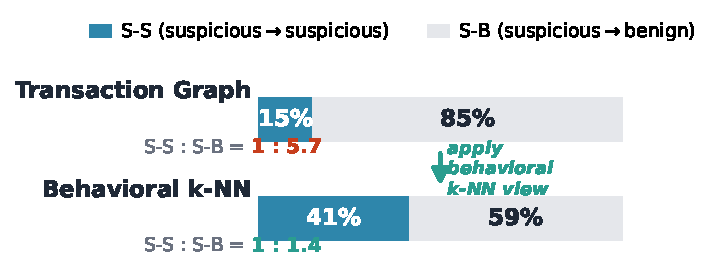
\includegraphics[width=0.95\columnwidth]{figures/fig_intro_homophily.pdf}
    \Description{Ego-network visualization.}
    \caption{Ego-network of a suspicious account on HOFINET. In the transaction graph only $\sim$15\% of neighbors are suspicious (S-S:S-B $=$ 1:5.7; S=suspicious, B=benign); the behavioral k-NN view ($k{=}10$) restores the S-S share to $\sim$41\% (S-S:S-B $=$ 1:1.4).}
    \label{fig:intro_homophily}
\end{figure}

\iffalse
그 첫 번째 특성은 저동질성 (low-homophily) 이다. 자금 세탁 계좌는 탐지 회피를 위해 의도적으로 정상 계좌와 거래하여 mule-network를 형성한다. 본 논문에서 사용한 한국의 은행 간 이체 결제망 Home/Firm Banking Network (HOFINET) 기반 합성 데이터 거래 그래프에서는 의심 계좌 이웃의 약 85\% 가 정상 계좌이다 (S-S:S-B $=$ 1:5.7\footnote{S-S:S-B 는 의심 계좌 주변에서 관측되는 \emph{의심--의심} : \emph{의심--정상} 엣지 비율이다. 동질성 $h(\mathcal{G})$ 는 전체 엣지 중 양 끝 노드 라벨이 같은 비율(=edge homophily)로 정의한다.}, Figure~\ref{fig:intro_homophily}). 이러한 구조에서는 표준 GNN의 핵심 가정인 이웃 라벨 유사성~\cite{zhu2020beyond} 이 성립하기 어렵고, 더 근본적으로는 의심--의심 이웃 신호 자체가 구조적으로 희소하다. H2GCN~\cite{zhu2020beyond}, FAGCN~\cite{bo2021beyond}, GBK-GNN~\cite{du2022gbk} 등 architecture 수준의 보강은 그래프 구조를 그대로 둔 채 message passing만 수정하므로, 이웃에 의심 신호가 거의 없는 거래 네트워크에서는 동질성 결함을 근본적으로 해소하지 못한다.
\fi
The first challenge is low homophily. Money-laundering accounts deliberately interact with benign accounts to evade detection, forming mule-networks. On a synthetic transaction graph built from HOFINET, a Korean inter-bank transfer settlement network, about 85\% of the neighbors of suspicious accounts are benign (S-S:S-B $=$ 1:5.7, Figure~\ref{fig:intro_homophily}). In this regime, the standard GNN assumption that neighbors tend to share labels~\cite{zhu2020beyond} is weak, and the core difficulty is that same-class (suspicious--suspicious) neighborhood evidence is structurally scarce to begin with. Architecture-level remedies such as H2GCN~\cite{zhu2020beyond}, FAGCN~\cite{bo2021beyond}, and GBK-GNN~\cite{du2022gbk} adjust message passing while leaving the graph itself unchanged, and therefore do not directly repair the homophily gap when few suspicious signals exist among the neighbors.

\iffalse
둘째와 셋째는 모두 학습에 활용할 라벨을 충분히 확보하기 어렵다는 점에서 맞물려 있다. 의심 계좌는 전체의 2\% 미만에 불과한 데다~\cite{hilal2022financial}, 라벨 역시 수사기관과 금융기관의 사후 조사 결과에 의존하므로 6개월 이상의 지연이 발생한다\cite{fatf2013guidance,kofia2024aml}. 이로 인해 CARE-GNN~\cite{dou2020enhancing}, PC-GNN~\cite{liu2021pick}, RioGNN~\cite{peng2021reinforced} 등 fraud-specific 지도학습 모델은 운영 환경에서 cold-start 문제를 겪는다. 결국 거래 네트워크에서는 라벨 부족과 이웃 구조 내 신호 부족이 동시에 작용한다.
\fi
The next two challenges, class imbalance and label scarcity, are closely related. Suspicious accounts make up less than 2\% of all accounts~\cite{hilal2022financial}, and labels rely on retrospective investigations by regulatory and financial institutions, which typically take six months or longer\cite{fatf2013guidance,kofia2024aml}. As a result, fraud-specific supervised models such as CARE-GNN~\cite{dou2020enhancing}, PC-GNN~\cite{liu2021pick}, and RioGNN~\cite{peng2021reinforced} face cold-start issues in production. Transaction networks therefore suffer from limited labels and weak in-neighborhood suspicious signals at the same time.

\iffalse
이러한 한계를 보완하기 위해 Graph Contrastive Learning (GCL)은 라벨 없이 증강된 view 간 일관성을 학습함으로써 그래프 표현을 얻는 대안으로 주목받고 있다~\cite{you2020graph,velivckovic2018deep,thakoor2021large,bielak2022graph}. 표준 GCL은 보통 원 그래프의 엣지나 피처를 일부 제거하거나 마스킹하여 입력 그래프 수준의 여러 view를 만든다. 그러나 이러한 view는 원 그래프와 의미적으로 유사해야 하므로, 원 거래 그래프의 저동질성 결함을 view 단계에서 근본적으로 제거하기보다는 보존할 수밖에 없다. 각 view의 표현을 가깝게 학습하는 과정에서도 입력 그래프의 anti-homophily는 두 view에 모두 잔존한다~\cite{zhu2020deep,zhu2021graph,hassani2020contrastive}.
\fi
Graph Contrastive Learning (GCL) is well suited here because it learns graph representations without labels by enforcing consistency across augmented views~\cite{you2020graph,velivckovic2018deep,thakoor2021large,bielak2022graph}. Standard GCL creates multiple graph-level views by removing or masking edges or features, but these views are designed to stay semantically close to the original graph. As a result, they preserve, rather than mitigate, a transaction graph’s low homophily. Even if training pulls the two views’ representations together, the input graph’s anti-homophily persists in both~\cite{zhu2020deep,zhu2021graph,hassani2020contrastive}.

\iffalse
입력 그래프를 직접 변형하지 않는 GCL 변형도 있다. 예를 들어 AFGRL~\cite{lee2022augmentation} 과 SimGRACE~\cite{xia2022simgrace} 는 같은 그래프를 모델에 두 번 입력하되, dropout이나 모델 가중치 perturbation 때문에 서로 조금 다른 임베딩이 나오도록 하고 이를 두 view로 사용한다. 이러한 방식은 학습을 안정화하는 데 도움이 되지만, 의심 계좌가 정상 계좌에 둘러싸여 있는 거래 엣지 구조 자체를 바꾸지는 못한다.

한편 MLGCL~\cite{shang2023mlgcl} 과 GCPAL~\cite{lu2024graph} 은 k-NN view, 즉 피처 공간에서 서로 가까운 노드들을 새로 연결한 보조 그래프를 도입하지만, 모든 피처를 함께 사용하므로 원 거래 그래프의 연결 구조에서 계산된 피처까지 k-NN 구축에 반영될 수 있다. 그 결과 보조 view가 원 거래 그래프와 충분히 독립적이지 못해, 거래 그래프의 저동질성 결함을 효과적으로 분리하지 못할 수 있다. 따라서 보조 view를 어떤 피처로 구성할지와, 그 view를 어떤 수준에서 대조할지가 핵심 설계 문제가 된다.
\fi
Some GCL variants avoid modifying the input graph. AFGRL~\cite{lee2022augmentation} and SimGRACE~\cite{xia2022simgrace} feed the same graph into the model twice and use embedding differences from dropout or weight perturbation as two views. These schemes can stabilize training but leave the transaction edge structure unchanged, so suspicious accounts remain surrounded by benign ones.

In contrast, MLGCL~\cite{shang2023mlgcl} and GCPAL~\cite{lu2024graph} add a k-NN auxiliary graph connecting nodes that are close in feature space. Yet, because they use all features, those derived from the original graph’s connectivity also affect k-NN construction, tying the auxiliary view to the original structure and hindering the isolation of low homophily. This motivates two design choices: which features to use for the auxiliary view and at which level to contrast it.
\iffalse
본 논문은 이 설계 문제를 view 구성과 contrastive level 두 측면에서 다룬다. View 측면에서, 자금세탁 계좌는 분할 거래와 다단계 이체 같은 공통 수법을 사용하므로 행동적 거래 패턴 (금액 분포, 시간적 빈도, 거래 유형 엔트로피) 을 공유한다. 먼저 각 계좌와 행동적으로 가장 유사한 $k$개의 계좌를 찾고, 이들을 새 엣지로 연결해 보조 그래프를 구성한다. 이렇게 만든 보조 그래프에서는 의심 계좌끼리 자연스럽게 연결되어 거래 그래프에서 단절되어 있던 동질성이 view 수준에서 회복된다. Level 측면에서는, 개별 노드만 대조하는 대신 회복된 view에서 각 계좌와 그 이웃들을 하나의 서브그래프로 묶어 풀링함으로써 정상 거래에 희석되던 의심 행동 패턴을 더 안정적으로 포착할 수 있다. 즉, 서브그래프 풀링은 회복된 view와 결합될 때 의심 신호를 정상 noise 위로 증폭한다.
\fi
We refine our approach along two axes: view construction and contrastive level. For view construction, money-laundering accounts share tactics such as structuring and layering, and thus often exhibit similar behavioral transaction patterns (amount distribution, temporal frequency, transaction-type entropy). For each account, we select the top $k$ most behaviorally similar accounts and connect them with new edges to form an auxiliary graph, where suspicious accounts are more likely to link to each other, restoring homophily at the view level. For the contrastive level, instead of using individual nodes, we group each account with its neighbors in this recovered view into a subgraph and pool over it, preserving suspicious behavior patterns that might otherwise be diluted by benign transactions.

\iffalse
이상의 논의를 바탕으로 본 논문은 \method 을 제안한다 (Figure~\ref{fig:framework}). \method 은 원 거래 그래프의 구조적 편향이 보조 view에 다시 반영되지 않도록 거래 구조 피처와 행동 피처를 분리하고, 행동 피처만으로 k-NN 보조 view를 구성한다. 이어서는 회복된 view에서 각 계좌의 이웃 집합을 서브그래프로 풀링하여 정상 이웃에 희석되었던 의심 신호를 증폭한다. 이러한 동질성 회복과 신호 증폭 메커니즘은 degree-corrected stochastic block model (DCSBM)~\cite{karrer2011stochastic} 에 기반해 이론적으로 분석된다. 또한 HOFINET, AMLworld~\cite{amlpatterns2024realistic}, AMLNet 세 데이터셋에서 행동적 k-NN view가 S-S:S-B 비율을 1:5.7에서 1:1.4로 개선하며, edge homophily는 transaction graph에서 0.690, behavioral view에서는 0.981로 나타나는 패턴을 확인한다. 본 연구의 기여는 다음과 같다.
\fi
We propose \method (Figure~\ref{fig:framework}), which separates structural transaction features from behavioral features so that the auxiliary view is based on behavioral similarity rather than the original graph topology. It then pools each account and its neighbors on the recovered view into a subgraph, preserving suspicious signals that would otherwise be diluted by benign neighbors. We analyze this homophily-recovery and signal-amplification mechanism with a degree-corrected stochastic block model (DCSBM)~\cite{karrer2011stochastic}. On HOFINET, the behavioral k-NN view improves the S-S:S-B ratio from 1:5.7 to 1:1.4, and edge homophily increases from 0.690 on the transaction graph to 0.981 on the behavioral view; the same qualitative pattern holds on AMLworld~\cite{amlpatterns2024realistic} and AMLNet. Our contributions are summarized below.
\iffalse
\begin{itemize}
    \item \textbf{행동 피처 기반 보조 view를 통한 graph-level 동질성 회복.} 거래 구조 피처와 행동 피처를 분리하고, 행동 피처만으로 k-NN 보조 view를 구성함으로써 원 거래 그래프의 저동질성 결함을 view 수준에서 완화한다. HOFINET에서 edge homophily는 transaction graph에서 0.690, behavioral k-NN view에서는 0.981로 나타나며, 회복 정도의 정량적 하한을 §\ref{subsec:theory} 에서 제시한다.
    \item \textbf{라벨 지연 및 cold-start AML 환경에서의 자기지도 학습 검증.} 의심 계좌 비율이 서로 다른 세 벤치마크 (2.13\% / 1.23\% / 13.52\%) 에서 \method 가 fully-supervised baseline과 경쟁적인 성능을 보이며, 1\% 라벨 cold-start에서도 $F1_{\text{susp}}{=}0.654$를 유지한다. 이는 라벨이 수사 기관의 사후 조사에 의존하는 실제 AML 운영 환경에서 라벨 없는 표현 학습의 실용성을 보여준다.
    \item \textbf{View 구성과 대조 수준의 역할 분해.} graph view (transaction view vs. auxiliary k-NN view) 와 contrastive level (노드 vs. 서브그래프) 두 축을 교차한 4가지 설정을 10종 GCL 인코더에 적용해, 동질성 회복은 보조 view 구성에서, 의심 신호 증폭은 회복된 view 위의 서브그래프 풀링에서 발생함을 보인다. 관련 메커니즘은 DCSBM 기반 분석과 BatchNorm collapse 정식화로 뒷받침한다.
\end{itemize}
\fi
\begin{itemize}
    \item \textbf{Recovering graph-level homophily via a behavioral perspective.} By separating structural and behavioral transaction features and building the k-NN auxiliary view only from behavioral features, \method mitigates low homophily in the original transaction graph. On HOFINET, edge homophily increases from 0.690 on the transaction graph to 0.981 on the behavioral k-NN view, with a quantitative lower bound in §\ref{subsec:theory}.
    \item \textbf{Self-supervised learning for delayed labels and AML cold start.} Across three datasets with suspicious-account prevalences of 2.13\%, 1.23\%, and 13.52\%, \method matches fully supervised baselines; in a 1\%-label cold-start regime, it still achieves $F1_{\text{susp}}{=}0.654$. This shows that label-free representation learning remains robust even when AML labels come only from retrospective investigations.
    \item \textbf{Decomposing graph view construction and contrastive level.} Crossing two axes (graph view: transaction view vs. auxiliary k-NN view; contrastive level: node vs. subgraph) into four settings and applying them to ten GCL encoders, we find that auxiliary graph view construction drives homophily recovery, while subgraph pooling on the recovered view amplifies suspicious signals. A DCSBM-based analysis and a formal characterization of BatchNorm collapse support these mechanisms.
\end{itemize}


\begin{figure*}[t!]
\centering
\scalebox{0.79}{
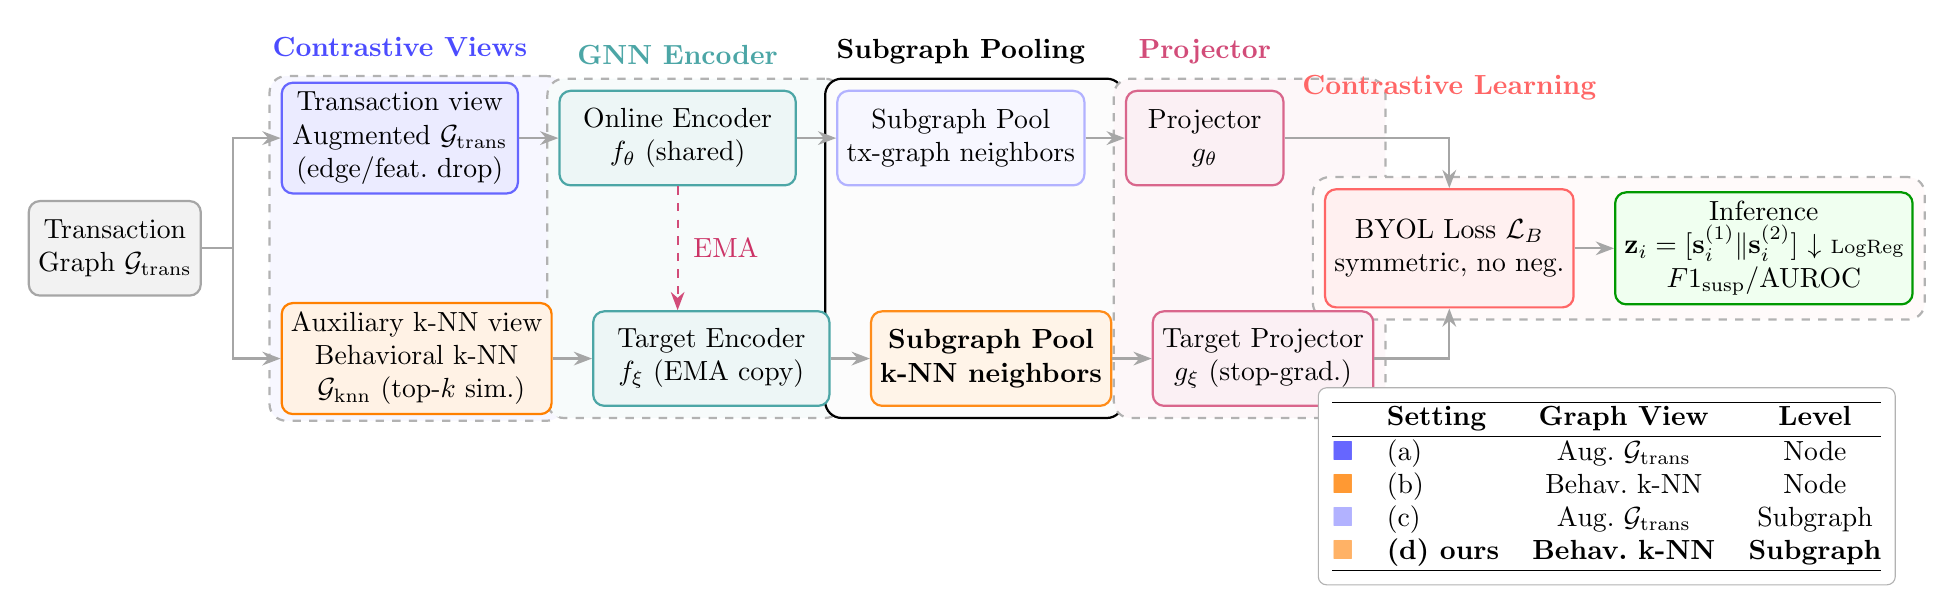
\begin{tikzpicture}[
  scale=1.0, transform shape, >=Stealth,
  node distance=0.4cm and 0.6cm,
  inputbox/.style={
    draw=gray!70, fill=gray!10, rounded corners=4pt,
    minimum width=2.0cm, minimum height=1.2cm, align=center, thick
  },
  viewbox/.style={
    draw, rounded corners=4pt,
    minimum width=3.0cm, minimum height=1.2cm, align=center, thick
  },
  view1/.style={viewbox, draw=blue!60, fill=blue!8},
  view2/.style={viewbox, draw=orange!100, fill=orange!10},
  encbox/.style={
    draw=teal!70, fill=teal!7, rounded corners=4pt,
    minimum width=3.0cm, minimum height=1.2cm, align=center, thick
  },
  poolbox_oth/.style={
    draw=blue!30, fill=blue!3, rounded corners=4pt,
    minimum width=3.0cm, minimum height=1.2cm, align=center, thick
  },
  poolbox_our/.style={
    draw=orange!90, fill=orange!9, rounded corners=4pt,
    minimum width=3.0cm, minimum height=1.2cm, align=center, thick
  },
  projbox/.style={
    draw=purple!60, fill=purple!6, rounded corners=4pt,
    minimum width=2.0cm, minimum height=1.2cm, align=center, thick
  },
  lossbox/.style={
    draw=red!60, fill=red!6, rounded corners=4pt,
    minimum width=2.0cm, minimum height=1.5cm, align=center, thick
  },
  infbox/.style={
    draw=green!60!black, fill=green!6, rounded corners=4pt,
    minimum width=2.0cm, align=center, thick
  },
  secbox/.style={
    draw=black!30, dashed, rounded corners=6pt,
    inner sep=8pt, thick
  },
  myarrow/.style={->, thick, gray!70},
  emaarrow/.style={->, thick, purple!70, dashed},
]
% --- COLUMN 1: Input ---
\node[inputbox] (txgraph) {Transaction\\Graph $\mathcal{G}_{\text{trans}}$};
% --- COLUMN 2: Contrastive views ---
\node[view1, right=1.0cm of txgraph, yshift=+1.4cm] (v1)
  {Transaction view\\{Augmented $\mathcal{G}_{\text{trans}}$}\\{(edge/feat.\ drop)}};
\node[view2, right=1.0cm of txgraph, yshift=-1.4cm] (v2)
  {Auxiliary k-NN view\\{Behavioral k-NN}\\{ $\mathcal{G}_{\text{knn}}$ (top-$k$ sim.)}};
\draw[myarrow] (txgraph.east) -- ++(0.4,0) |- (v1.west);
\draw[myarrow] (txgraph.east) -- ++(0.4,0) |- (v2.west);
\node[above=0.2cm of v1, font=\bfseries, text=blue!70] (lv) {Contrastive Views};
% --- COLUMN 3: Encoders ---
\node[encbox, right=0.5cm of v1] (enc1)
  {Online Encoder\\$f_\theta$ (shared)};
\node[encbox, right=0.5cm of v2] (enc2)
  {Target Encoder\\$f_\xi$ (EMA copy)};
\draw[myarrow] (v1.east) -- (enc1.west);
\draw[myarrow] (v2.east) -- (enc2.west);
\draw[emaarrow] (enc1.south) -- node[pos=0.5, right=2pt, text=purple!80]{EMA} (enc2.north -| enc1.south);
\node[above=0.2cm of enc1, font=\bfseries, text=teal!70] {GNN Encoder};
% --- COLUMN 4: Subgraph Pool ---
\node[poolbox_oth, right=0.5cm of enc1] (pool1)
  {Subgraph Pool\\{tx-graph neighbors}};
\node[poolbox_our, right=0.5cm of enc2] (pool2)
  {\textbf{Subgraph Pool}\\\textbf{k-NN neighbors}};
\draw[myarrow] (enc1.east) -- (pool1.west);
\draw[myarrow] (enc2.east) -- (pool2.west);
\node[above=0.2cm of pool1, font=\bfseries, text=black] {Subgraph Pooling};
% --- COLUMN 5: Projectors ---
\node[projbox, right=0.5cm of pool1] (proj1)
  {Projector\\$g_\theta$};
\node[projbox, right=0.5cm of pool2] (proj2)
  {Target Projector\\$g_\xi$ (stop-grad.)};
\draw[myarrow] (pool1.east) -- (proj1.west);
\draw[myarrow] (pool2.east) -- (proj2.west);
\node[above=0.2cm of proj1, font=\bfseries, text=purple!70] {Projector};
% --- COLUMN 6: Loss + Inference ---
\node[lossbox, right=0.5cm of proj1, yshift=-1.4cm] (loss)
  {BYOL Loss $\mathcal{L}_B$\\{symmetric, no neg.}};
\draw[myarrow] (proj1.east) -| (loss.north);
\draw[myarrow] (proj2.east) -| (loss.south);
\node[infbox, right=0.5cm of loss] (inf)
  {Inference\\
    $\mathbf{z}_i=[\mathbf{s}_i^{(1)}\|\mathbf{s}_i^{(2)}]$
    $\downarrow$ {\scriptsize LogReg}\\
    {$F1_{\text{susp}}$/AUROC}};
\draw[myarrow] (loss.east) -- (inf.west);
\node[above=0.2cm of loss, yshift=0.8cm, font=\bfseries, text=red!60] {Contrastive Learning};
% --- Background boxes ---
\begin{scope}[on background layer]
  \node[secbox, fit=(v1)(v2), fill=blue!3, inner xsep=4pt, inner ysep=2pt] {};
  \node[secbox, fit=(enc1)(enc2), fill=teal!3, inner xsep=4pt, inner ysep=4pt] {};
  \node[secbox, fit=(pool1)(pool2), draw=black, solid, fill=gray!2, inner xsep=4pt, inner ysep=4pt] {};
  \node[secbox, fit=(proj1)(proj2), fill=purple!3, inner xsep=4pt, inner ysep=4pt] {};
  \node[secbox, fit=(loss)(inf), fill=red!2, inner xsep=4pt, inner ysep=4pt] {};
\end{scope}
% --- Ablation table ---
\node[below=1.0cm of loss, xshift=2.0cm,
  draw=black!30, rounded corners=3pt, inner sep=5pt,
  fill=white] (abltbl) {
  \begin{tabular}{@{}clcc@{}}
    \hline
    & \textbf{Setting} & \textbf{Graph View} & \textbf{Level} \\
    \hline
    {\color{blue!60}$\blacksquare$} & (a) & Aug.\ $\mathcal{G}_{\text{trans}}$ & Node \\
    {\color{orange!80}$\blacksquare$} & (b) & Behav.\ k-NN & Node \\
    {\color{blue!30}$\blacksquare$} & (c) & Aug.\ $\mathcal{G}_{\text{trans}}$ & Subgraph \\
    {\color{orange!60}$\blacksquare$} & \textbf{(d) ours} & \textbf{Behav.\ k-NN} & \textbf{Subgraph} \\
    \hline
  \end{tabular}
};
\end{tikzpicture}
}% end resizebox
    \caption{Overview of \method. We construct two contrastive views: (i) an augmented transaction view (stochastic perturbations of $\mathcal{G}_{\text{trans}}$) and (ii) a behavioral k-NN auxiliary view. The two views are encoded with a shared online GNN $f_\theta$ and its EMA target copy $f_\xi$, and trained with a symmetric BYOL-style bootstrap loss (no negatives). The representation level depends on the setting: (a)(b) contrast node embeddings, while (c)(d) apply subgraph pooling before contrast. Bottom legend: 4-setting ablation; (d) is the proposed configuration.}
    \label{fig:framework}
\end{figure*}

\section{Related Work}\label{sec:related_work}
% Korean drafts below are kept inside \iffalse blocks for reference and are not compiled.
\iffalse
\subsection{저동질성 그래프 학습}
H2GCN~\cite{zhu2020beyond}, Geom-GCN~\cite{pei2020geom}, FAGCN~\cite{bo2021beyond}, GBK-GNN~\cite{du2022gbk}, ACM-GCN~\cite{luan2022acmgcn}, GPR-GNN~\cite{chien2021adaptive}, LINKX~\cite{zhu2021linkx} 등 저동질성 대응 GNN은 ego와 이웃 임베딩을 분리하고, propagation channel을 조정하며, 구조와 속성을 분리 처리 등을 통해 low-homophily 환경에서의 message passing을 개선한다. 그러나 이들 방법은 기본적으로 주어진 그래프 구조를 유지한 채 집계 방식을 조정한다. AML 거래 네트워크에서는 의심 계좌가 탐지 회피를 위해 정상 계좌와 의도적으로 거래하므로, 집계 가능한 의심-의심 이웃 엣지 자체가 부족하다. 따라서 propagation 수준의 보강만으로는 부족한 same-class neighborhood를 회복하기 어렵다. 본 연구는 거래 행동(금액/시간/유형 통계)이 유사한 의심 계좌들이 서로 연결될 수 있도록 대조 학습에 사용하는 view를 행동 기반 k-NN 보조 그래프로 새로 구성한다.
\fi
\subsection{Low-homophily / heterophily-aware graph learning}
Heterophily-aware GNN such as H2GCN~\cite{zhu2020beyond}, Geom-GCN~\cite{pei2020geom}, FAGCN~\cite{bo2021beyond}, GBK-GNN~\cite{du2022gbk}, ACM-GCN~\cite{luan2022acmgcn}, GPR-GNN~\cite{chien2021adaptive}, and LINKX~\cite{zhu2021linkx} improve message passing under low homophily by separating ego and neighbor embeddings, adjusting propagation channels, or decoupling structure from attributes. These methods adjust how aggregation is performed while keeping the input graph fixed. In AML transaction networks, suspicious accounts deliberately transact with benign ones to evade detection, making suspicious-to-suspicious neighbor edges rare. Propagation-level remedies alone are unlikely to restore the missing same-class neighborhood. We instead build the contrastive view as a behavior-based k-NN auxiliary graph so that suspicious accounts with similar transaction behavior become directly connected.

\iffalse
\subsection{그래프 대조학습과 view 구성}
Graph Contrastive Learning (GCL)은 여러 view 간 일관성을 학습하여 그래프 표현을 얻는 대표적인 자기지도 학습 방법이다. 그러나 DGI~\cite{velivckovic2018deep}, GRACE~\cite{zhu2020deep}, GraphCL~\cite{you2020graph}, GCA~\cite{zhu2021graph}, BGRL~\cite{thakoor2021large}, GBT~\cite{bielak2022graph}, MVGRL~\cite{hassani2020contrastive} 등은 대체로 동일 입력 그래프에 확률적 perturbation을 적용하여 view를 구성한다. AFGRL~\cite{lee2022augmentation}, SimGRACE~\cite{xia2022simgrace}, CCA-SSG~\cite{zhang2021canonical}, GraphMAE~\cite{hou2022graphmae}, S2GAE~\cite{li2023s2gae} 등 augmentation-free 변형은 명시적 그래프 증강을 사용하지 않지만, view를 거래 엣지 구조의 보정이 아니라 표현 또는 모델 수준에서 생성한다. 따라서 입력 거래 그래프가 anti-homophilous한 경우, 기존 GCL의 view는 저동질성 구조를 완화하기보다 그대로 유지될 가능성이 크다. 본 연구는 거래 행동의 유사성에 기반한 보조 그래프를 한쪽 view로 구성하여 graph 수준의 동질성을 회복하면서, GCL의 자기지도 학습 장점을 유지한다.
\fi
\subsection{GCL and view design}
Graph Contrastive Learning (GCL) is a self-supervised framework that derives graph representations by enforcing consistency across multiple views. Representative approaches, including DGI~\cite{velivckovic2018deep}, GRACE~\cite{zhu2020deep}, GraphCL~\cite{you2020graph}, GCA~\cite{zhu2021graph}, BGRL~\cite{thakoor2021large}, GBT~\cite{bielak2022graph}, and MVGRL~\cite{hassani2020contrastive}, typically obtain such views through stochastic perturbations of a single input graph. Augmentation-free approaches, including AFGRL~\cite{lee2022augmentation}, SimGRACE~\cite{xia2022simgrace}, CCA-SSG~\cite{zhang2021canonical}, GraphMAE~\cite{hou2022graphmae}, and S2GAE~\cite{li2023s2gae}, eliminate the need for explicit graph augmentations. However, they still generate views at the representation or model level, not by explicitly repairing the transaction edge structure. On anti-homophilous transaction graphs, their views thus preserve rather than alleviate low homophily. We instead use a behavioral-similarity auxiliary graph as one view, restoring homophily at the graph level while retaining the self-supervised benefits of GCL.

\iffalse
\subsection{Fraud GNN과 라벨 지연 문제}
GNN 기반 fraud 및 AML 모델은 fraud-aware 이웃 선택, 라벨 분포 기반 샘플링, reweighting, 시간 패턴 모델링, 다중 관계 추론 등을 통해 거래 네트워크 탐지 성능을 개선해 왔다\cite{liu2020alleviating,dou2020enhancing,liu2021pick,peng2021reinforced,zhang2021fraudre,cheng2020graph,rao2020xfraud,wang2023label,cheng2025graph}. 이러한 방법들은 라벨이 충분히 확보된 상황에서는 효과적이지만, 학습 시점에 의심 사례 라벨이 존재한다는 전제를 둔다. AML에서 의심 라벨은 사후 조사에 의존하므로 거래 발생 후 수개월이 지나서야 확정되는 경우가 많다. 따라서 실제 AML 운영에서는 의심 라벨이 확정되기 전에도 거래 네트워크로부터 자금세탁 의심 패턴을 모델링할 수 있는 방법이 필요하다. 이 때문에 AML에서는 라벨 없이 거래 표현을 먼저 학습하는 자기 지도/비지도 접근이 선택적 보강이 아니라 운영상 필요한 대안이 된다. 본 연구는 표현 학습 단계에서 라벨을 사용하지 않고, downstream 평가 head에서만 라벨을 사용함으로써 이러한 라벨 지연 문제를 완화한다.
\fi
\subsection{Fraud GNNs and label delay}
GNN-based fraud and AML models have improved detection on transaction networks through fraud-aware neighbor selection, label-distribution-based sampling, reweighting, temporal-pattern modeling, and multi-relation inference~\cite{liu2020alleviating,dou2020enhancing,liu2021pick,peng2021reinforced,zhang2021fraudre,cheng2020graph,rao2020xfraud,wang2023label,cheng2025graph}. These methods work well when labels are abundant, but they assume that suspicious labels are available at training time. In AML, suspicious labels depend on retrospective investigations and are often confirmed only several months after the transaction. In production AML settings, it is therefore desirable to model suspicious patterns from the transaction network even before such labels arrive. For this reason, label-free representation learning serves as a practical alternative under operational constraints rather than an optional enhancement. We use labels only at the downstream evaluation head, which mitigates this label-delay issue.

\iffalse
\subsection{비지도 graph anomaly detection}
DOMINANT~\cite{ding2019dominant}, CoLA~\cite{liu2021anomaly}, ANEMONE~\cite{jin2021anemone}, BWGNN~\cite{tang2022rethinking}, BOND~\cite{liu2022bond} 등 비지도 그래프 이상 탐지 연구는 노드 속성과 그래프 구조의 재구성 오차 또는 노드-서브그래프 대조 학습 등을 활용하여 이상 노드를 탐지해 왔다. 그러나 이들 방법은 주로 일반 그래프 벤치마크에서 검증되었으며, 라벨 지연, 낮은 prevalence, mule-network 기반 회피, 저동질성 거래 엣지가 동시에 나타나는 AML 거래 네트워크를 중심으로 설계되지 않았다. 본 연구는 이러한 AML 특성을 반영하여 행동 기반 view를 구성하고, 서브그래프 풀링이 의심 신호를 증폭하는 조건과 신호를 희석할 수 있는 조건을 함께 분석한다. 또한 극심한 클래스 불균형에서 발생하는 collapse 동작까지 다룬다. 더 넓은 비교는 Appendix~\ref{app:rw_extended}에 제시한다.
\fi
\subsection{Unsupervised graph anomaly detection}
Unsupervised graph anomaly detection methods such as DOMINANT~\cite{ding2019dominant}, CoLA~\cite{liu2021anomaly}, ANEMONE~\cite{jin2021anemone}, BWGNN~\cite{tang2022rethinking}, and BOND~\cite{liu2022bond} detect anomalous nodes through reconstruction errors in node attributes and graph structures, or through node-subgraph contrastive learning. These methods are primarily evaluated on general graph benchmarks and are not specifically designed for AML transaction networks, where label delay, low prevalence, mule-network-based evasion, and low-homophily transaction edges co-occur. We tailor the view to these AML characteristics by constructing it from behavioral features, and we analyze both when subgraph pooling amplifies suspicious signals and when it instead dilutes them. We also examine the collapse behavior that arises under severe class imbalance. A broader comparison is given in Appendix~\ref{app:rw_extended}.

\iffalse
\paragraph{k-NN view 기반 그래프 대조학습.}
MLGCL~\cite{shang2023mlgcl} 과 GCPAL~\cite{lu2024graph} 은 k-NN view를 명시적으로 도입한다는 점에서 본 연구와 가장 가깝다. AML 관점에서 중요한 쟁점은 k-NN 사용 여부 자체가 아니라, k-NN 그래프를 어떤 피처로 구성할 것인가이다. 모든 가용 피처를 함께 사용하면 degree나 centrality처럼 원 거래 그래프의 연결 구조에서 계산된 피처가 보조 그래프 구성에 다시 반영되어 거래 topology와 독립적인 보조 view를 만드는 것이 어렵다. 또한 기존 k-NN view 연구는 피처 선택 효과와 contrastive level 효과를 체계적으로 분리해 분석하지 않았다. 본 연구는 행동 피처만으로 k-NN view를 구성하고, view 구성 (거래 그래프 vs. 행동 k-NN) 과 contrastive level (노드 vs. 서브그래프) 을 교차한 4가지 설정을 통해 두 효과를 함께 검증한다.
\fi
\subsection{k-NN view based GCL}
MLGCL~\cite{shang2023mlgcl} and GCPAL~\cite{lu2024graph} are the closest prior works in that they explicitly introduce a k-NN view. From an AML perspective, the central issue is which features should define the k-NN view, not whether to use one. In our setting, we compute behavioral features from transaction behavior (amount, timing, and type statistics) rather than from graph connectivity, so the induced k-NN edges aim to be complementary to the transaction topology. Using all available features lets quantities computed from the original transaction connectivity, such as degree or centrality, leak back into the auxiliary graph, which makes it hard to obtain an auxiliary view that is independent of the transaction topology. Existing k-NN view studies also do not separate the effect of feature choice from the effect of contrastive level. We build the k-NN view from behavioral features alone and validate both effects jointly through four settings that cross view construction (transaction graph vs. behavioral k-NN) and contrastive level (node vs. subgraph).

\iffalse
종합하면, 기존 연구는 각각 저동질성 전파, 라벨 의존 탐지, 자기 지도 표현 학습, 비지도 이상 탐지, k-NN 기반 view 구성의 측면에서 중요한 진전을 이루었으나, AML 거래 네트워크에서 동시에 나타나는 세 조건, 즉 저동질성 거래 구조, 라벨 지연, 그리고 행동적으로 유사하지만 거래상으로는 분리된 의심 계좌를 함께 충족하는 접근은 제한적이다. 본 연구는 이 공백을 메우기 위해 행동 피처 기반 보조 view를 구성하고, 그 위에서 서브그래프 수준 대조 학습을 수행하며, view 구성과 contrastive level의 효과를 이론 분석과 대규모 실험으로 분리 검증한다.
\fi
Taken together, prior work has made progress on heterophilous propagation, label-dependent detection, self-supervised representation learning, unsupervised anomaly detection, and k-NN based view construction; however, few approaches simultaneously address the three conditions that co-occur in AML transaction networks: low-homophily transaction structure, label delay, and suspicious accounts that are behaviorally similar yet transactionally disconnected. We aim to fill this gap by constructing a behavioral-feature-based auxiliary view, performing subgraph-level contrastive learning on it, and separately validating the effects of view construction and contrastive level through theoretical analysis and large-scale experiments.

\section{Method: \method}
\label{sec:method}

\subsection{Problem Formulation}
\iffalse
거래 네트워크를 유향 그래프 $\mathcal{G}_{\text{trans}} = (\mathcal{V}, \mathcal{E}, \mathbf{X})$로 정의한다.
$\mathcal{V}$는 계좌(노드) 집합($|\mathcal{V}|=N$), $\mathcal{E} \subseteq \mathcal{V} \times \mathcal{V}$는 이체 거래(간선) 집합, $\mathbf{X} \in \mathbb{R}^{N \times F}$는 노드 특성 행렬이다.
각 노드 $v_i$에는 의심 여부를 나타내는 라벨 $y_i \in \{0, 1\}$이 있지만, 학습 단계에서는 라벨을 사용하지 않는 자기지도 설정을 따른다.
목표는 라벨 없이 그래프 구조와 노드 특성으로부터 의심 계좌를 식별할 수 있는 노드 표현 $\mathbf{Z} \in \mathbb{R}^{N \times D}$을 학습하는 것이다.
\fi
We model the transaction network as a directed graph $\mathcal{G}_{\text{trans}} = (\mathcal{V}, \mathcal{E}, \mathbf{X})$, where $\mathcal{V}$ is the set of accounts (nodes, $|\mathcal{V}|=N$), $\mathcal{E} \subseteq \mathcal{V} \times \mathcal{V}$ is the set of transfer transactions (edges), and $\mathbf{X} \in \mathbb{R}^{N \times F}$ is the node feature matrix. Each node $v_i$ carries a suspicion label $y_i \in \{0, 1\}$, but we adopt a self-supervised setting that does not use labels during training. The goal is to learn node representations $\mathbf{Z} \in \mathbb{R}^{N \times D}$ that identify suspicious accounts from the graph structure and node features alone.

\subsection{Feature Taxonomy}
\label{subsec:feature_taxonomy}
\iffalse
거래 네트워크에서 추출 가능한 노드 특성을 행동 특성, 그래프 파생 특성, 구조 특성으로 구분한다(Table~\ref{tab:features}).
\fi
We group the node features available in a transaction network into behavioral, network-derived, and structural categories (Table~\ref{tab:features}).

\begin{table}[!ht]
\centering
\caption{Node feature taxonomy. Behavioral and network-derived features are used as GNN input, while k-NN view construction uses only 20 behavioral variables.}
\label{tab:features}
\resizebox{\columnwidth}{!}{%
\begin{tabular}{llrcc}
\toprule
\textbf{Category} & \textbf{Features} & \textbf{\#} & \textbf{GNN} & \textbf{k-NN} \\
\midrule
\multicolumn{2}{l}{\textit{\textbf{Behavioral}}} & \textit{Total} - 20 & & \\
\midrule
\textbf{Amount stats}     & \makecell[l]{\text{in\_mean, in\_max, in\_std}\\\text{out\_mean, out\_max, out\_std}} & 6 & \checkmark & \checkmark \\
\textbf{Temporal (3min)}    & \makecell[l]{\text{in\_3m\_mean, in\_3m\_count}\\\text{out\_3m\_mean, out\_3m\_count}} & 2 & \checkmark & \checkmark \\
\textbf{Temporal (6min)}    & \makecell[l]{\text{in\_6m\_mean, in\_6m\_count}\\\text{out\_6m\_mean, out\_6m\_count}} & 2 & \checkmark & \checkmark \\
\textbf{Temporal (12min)}   & \makecell[l]{\text{in\_12m\_mean, in\_12m\_count}\\\text{out\_12m\_mean, out\_12m\_count}} & 2 & \checkmark & \checkmark \\
\textbf{Entropy}          & \makecell[l]{\text{md\_type\_entropy, fnd\_type\_entropy}} & 2 & \checkmark & \checkmark \\
\midrule
\multicolumn{2}{l}{\textit{Network-derived}} & \textit{Total} - 4 & & \\
\midrule
Count            & out\_count, in\_count            & 2 & \checkmark &  \\
Degree           & in\_dc, out\_dc                  & 2 & \checkmark &  \\
\midrule
\multicolumn{2}{l}{\textit{Structural}} & \textit{Total} - 7 & & \\
\midrule
Centrality       & dc, pagerank, betweenness        & 3 &  &  \\
Hub/Authority    & hits\_hub, hits\_auth             & 2 &  &  \\
Topology         & kcore, triangle                  & 2 &  &  \\
\bottomrule
\end{tabular}}
\end{table}

\iffalse
행동 특성은 거래 금액 통계, 시간대별 빈도, 거래 유형 엔트로피(Table~\ref{tab:features})로 구성되어 거래 패턴을 나타낸다. 그래프 파생 특성(거래 건수, 차수)은 인코더 입력에는 포함하지만 k-NN view 구성에는 사용하지 않는다. 구조 특성(중심성, 허브/권한도, 위상)은 분석과 보조 비교에만 사용한다. 이하에서 $\mathbf{X}^{\text{enc}}$는 GNN 인코더 입력으로 사용하는 행동 및 그래프 파생 특성 행렬을, $\mathbf{X}^{\text{knn}}$는 k-NN 구축에 사용하는 20개 행동 특성 행렬을 의미한다. 의심 계좌들이 탐지 회피를 위해 정상 계좌와 의도적으로 거래하면 거래 그래프에서 저동질성 문제가 발생한다. \method는 이를 완화하기 위해 유사한 행동을 하는 계좌들이 서로 연결될 수 있도록, 대조 학습에 사용하는 view를 행동 기반 k-NN 보조 그래프로 새로 구성한다.
\fi
The behavioral features summarize transaction patterns through amount statistics, time-window frequencies, and transaction-type entropies (Table~\ref{tab:features}). The network-derived features (transaction counts and degrees) are fed into the encoder but are not used in the k-NN view, and the structural features (centrality, hub/authority, and topology) are used only for analysis and auxiliary comparisons. In what follows, $\mathbf{X}^{\text{enc}}$ denotes the behavioral and network-derived features given to the GNN encoder, and $\mathbf{X}^{\text{knn}}$ denotes the $20$ behavioral features used to build the k-NN graph. When suspicious accounts deliberately transact with benign ones to avoid detection, the transaction graph becomes low-homophily. We address this by constructing the contrastive view as a behavioral k-NN auxiliary graph so that accounts with similar behavior can be linked even when they are not directly connected in transactions.

\subsection{Behavioral k-NN View}
\label{subsec:knn_view}
\iffalse
\method의 핵심은 행동 유사도 기반 k-NN 그래프를 거래 엣지와 별도로 구축하는 것이다. 표준적인 증강 기반 GCL이 원 그래프의 엣지 제거나 피처 마스킹을 통해 대조 입력을 생성하는 반면, \method는 거래 그래프 $\mathcal{G}_{\text{trans}}$의 엣지 구조와 별도로 구성한 k-NN 그래프를 auxiliary k-NN view로 활용한다(Figure~\ref{fig:framework}의 auxiliary graph view).

\textbf{k-NN 그래프 구축.} 먼저 행동 변수 $\mathbf{x}_i^{\text{knn}} \in \mathbb{R}^{20}$의 스케일 차이를 제거하기 위해 평균이 0이고 분산이 1이 되도록 표준화한 후, 벡터의 방향에 기반한 유사도 계산을 위하여 L2 정규화를 적용한다:
\fi
A central component of \method is a behavioral-similarity k-NN graph built separately from the transaction edges. Standard augmentation-based GCL produces contrastive inputs by dropping edges or masking features on the original graph. We instead use a k-NN graph that is constructed independently of the edge structure of $\mathcal{G}_{\text{trans}}$ as an auxiliary k-NN view (auxiliary graph view in Figure~\ref{fig:framework}).

\textbf{k-NN graph construction.} We first standardize the behavioral features $\mathbf{x}_i^{\text{knn}} \in \mathbb{R}^{20}$ to have a zero mean and unit variance to remove scale differences across variables, and then apply L2 normalization so that similarity depends on the direction of the feature vector:

\begin{equation}
\label{eq:l2norm}
    \bar{\mathbf{x}}_i = \text{StandardScaler}(\mathbf{x}_i^{\text{knn}}), \quad
    \tilde{\mathbf{x}}_i = \frac{\bar{\mathbf{x}}_i}{\|\bar{\mathbf{x}}_i\|_2}
\end{equation}

\iffalse
L2 정규화된 두 벡터에 대해서는 유클리드 거리 순위가 코사인 유사도 순위와 단조적으로 대응하므로, 본 연구에서는 유클리드 거리 기반의 ball tree 탐색을 통해 각 노드 $v_i$의 $k$개 최근접 이웃을 찾는다. 이를 연결하여 k-NN 그래프 $\mathcal{G}_{\text{knn}} = (\mathcal{V}, \mathcal{E}_{\text{knn}})$를 구축한다.
\fi
Because the Euclidean distance between two L2-normalized vectors is monotonic in their cosine similarity, we retrieve the $k$ nearest neighbors of each node $v_i$ with a ball-tree search over Euclidean distance. Connecting each node to these neighbors yields the k-NN graph $\mathcal{G}_{\text{knn}} = (\mathcal{V}, \mathcal{E}_{\text{knn}})$:

\begin{equation}
\label{eq:knn_edge}
    \mathcal{E}_{\text{knn}} = \{(v_i, v_j) \mid v_j \in \text{kNN}(v_i, k)\}.
\end{equation}

We use the symmetrized (bidirected) version of this k-NN graph for message passing and pooling, i.e., we add $(v_j, v_i)$ whenever $(v_i, v_j) \in \mathcal{E}_{\text{knn}}$.

\iffalse
여기서 $\text{kNN}(v_i, k)$는 $\tilde{\mathbf{x}}_i$와의 유클리드 거리가 가장 가까운 $k$개 노드 집합이며, 본 연구에서는 $k=10$을 기본값으로 사용한다. 또한 message passing 및 풀링에는 k-NN 그래프를 대칭화하여 사용한다(즉, $(v_i,v_j)$가 있으면 $(v_j,v_i)$도 추가).

자금세탁 계좌들은 자금 분할 거래와 다단계 이체 과정에서 금액 분포, 시간대별 거래 빈도, 거래 유형 엔트로피 등에서 유사한 행동 패턴을 보일 수 있다. 따라서 행동 유사도 기반 k-NN은 거래 그래프에서 직접 연결되지 않은 의심 계좌들도 보조 view에서 가까운 이웃으로 연결될 가능성을 높이며, 이를 통해 거래 그래프의 저동질성으로 인해 부족했던 의심--의심 이웃 구조를 view 수준에서 보완한다.
\fi
Here, $\text{kNN}(v_i, k)$ is the set of $k$ nodes with the smallest Euclidean distance to $\tilde{\mathbf{x}}_i$, and we use $k=10$ as the default.

Money-laundering accounts that split transactions and layer transfers often share similar behavior in amount distributions, time-window frequencies, and transaction-type entropies. A behavioral k-NN graph, therefore, tends to link suspicious accounts that are not directly connected in transactions, restoring the suspicious-to-suspicious neighborhood structure missing from the low-homophily transaction view.

\subsection{Dual-View GNN Encoder}
\label{subsec:dual_view}
\iffalse
Dual-view 대조 학습의 핵심은 거래 구조를 담은 transaction view와 행동 유사성을 담은 auxiliary k-NN view를 같은 계좌 기준으로 정렬하는 것이다. 본 연구에서 graph view는 원천 그래프(source graph)에 간선 제거와 특성 마스킹을 적용해 만든 대조 학습 입력을 의미한다. \method는 원 거래 그래프 $\mathcal{G}_{\text{trans}}$에서 만든 transaction view와, 행동 기반 k-NN 그래프 $\mathcal{G}_{\text{knn}}$에서 만든 auxiliary k-NN view를 함께 사용한다.
\fi
Dual-view contrastive learning aligns a transaction view, which carries the transaction structure, and an auxiliary k-NN view, which carries behavioral similarity, around the same account. In our setting, a graph view is the contrastive input obtained by applying edge dropping and feature masking to a source graph. \method uses the transaction view derived from $\mathcal{G}_{\text{trans}}$ together with the auxiliary k-NN view derived from $\mathcal{G}_{\text{knn}}$.

\begin{figure}[H]
\centering
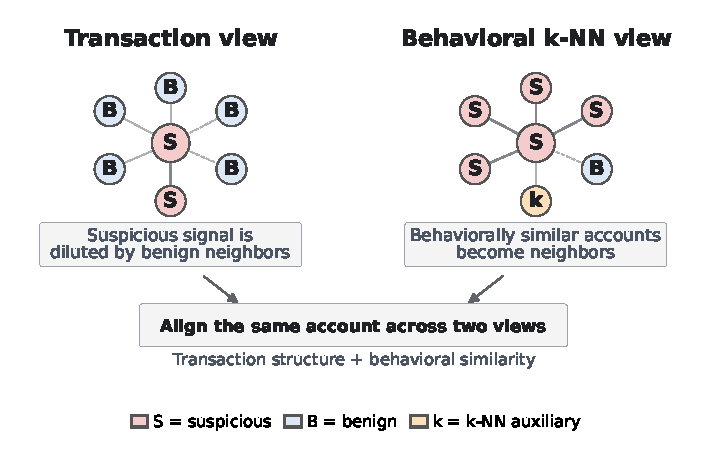
\includegraphics[width=\columnwidth]{figures/fig_dual_view_motivation.pdf}
\caption{Motivation for dual-view contrastive learning. The transaction view preserves real fund-flow structure but can dilute suspicious signals through benign neighbors. The behavioral k-NN view connects behaviorally similar suspicious accounts as auxiliary neighbors, and \method aligns the same account across the two views to learn both sources of information.}
\Description{A schematic comparing the transaction view and the behavioral k-NN view. The transaction view connects a suspicious account mostly to benign accounts, while the behavioral k-NN view connects it to behaviorally similar suspicious accounts. A contrastive learning block aligns the same account across both views.}
\label{fig:dual_view_motivation}
\end{figure}

\iffalse
\textbf{Contrastive Views.} Transaction view만 사용하면 의심 계좌의 표현이 주변 정상 계좌에 의해 희석되고, auxiliary k-NN view만 사용하면 실제 거래 관계의 구조 정보가 사라진다(Figure~\ref{fig:dual_view_motivation}). 이에 \method 은 두 view에서 같은 계좌의 표현을 일관되게 학습하여 실제 거래 구조와 행동 유사성을 함께 반영한다.

\textbf{GNN Encoder.} 원 거래 그래프와 보조 k-NN 그래프에 확률적 간선 제거와 특성 마스킹을 적용하여 두 그래프 뷰를 만든다. 증강 강도는 $p_e{=}p_f{=}0.3$으로 고정하고 모든 실험에 동일하게 적용한다. 이후 온라인 GNN 인코더 $f_\theta$를 두 view에 공유하여 임베딩 $\mathbf{H}^{(1)} = f_\theta(\mathbf{X}^{\text{enc}}, \tilde{\mathcal{E}}_{\text{trans}})$, $\mathbf{H}^{(2)} = f_\theta(\mathbf{X}^{\text{enc}}, \tilde{\mathcal{E}}_{\text{knn}})$을 생성한다. 목표 인코더 $f_\xi$는 같은 구조의 EMA copy로, BYOL 손실의 반대쪽 경로에서 stop-gradient 표현을 제공한다. 한 가지 구현 예로 온라인 GNN 인코더는 여러 개의 GCNConv~\cite{kipf2016semi} 층으로 구성되며, 각 층 뒤에는 학습 안정화를 위한 배치 정규화, 비선형 활성화 함수, 드롭아웃을 차례로 적용한다(상세는 부록~\ref{app:impl} 참조). \method 은 인코더에 무관하게 설계되어 GIN~\cite{xu2018powerful}, MVGRL, GBT 등 10가지 인코더와 호환되며, 배치 정규화의 역할은 Section~\ref{subsec:rq4}의 대조 실험으로 확인한다.
\textbf{GNN Encoder.} 원 거래 그래프와 보조 k-NN 그래프에 확률적 간선 제거와 특성 마스킹을 적용하여 두 graph view를 만든다. 증강 강도는 $p_e{=}p_f{=}0.3$으로 고정하고 모든 실험에 동일하게 적용한다. 이후 온라인 GNN 인코더 $f_\theta$를 두 view에 공유하여 임베딩 $\mathbf{H}^{(1)} = f_\theta(\mathbf{X}^{\text{enc}}, \tilde{\mathcal{E}}_{\text{trans}})$, $\mathbf{H}^{(2)} = f_\theta(\mathbf{X}^{\text{enc}}, \tilde{\mathcal{E}}_{\text{knn}})$을 생성한다. 목표 인코더 $f_\xi$는 같은 구조의 EMA copy로, BYOL 손실의 반대쪽 경로에서 stop-gradient 표현을 제공한다. 온라인 GNN 인코더는 여러 개의 GCNConv~\cite{kipf2016semi} 층으로 구성되며, 각 층 뒤에는 학습 안정화를 위한 배치 정규화, 비선형 활성화 함수, 드롭아웃을 차례로 적용한다(상세는 부록~\ref{app:impl} 참조). \method 은 인코더에 무관하게 설계되어 GIN~\cite{xu2018powerful}, MVGRL, GBT 등 10가지 인코더와 호환되며, 배치 정규화의 역할은 Section~\ref{subsec:rq2}의 대조 실험으로 확인한다.
\textbf{GNN Encoder.} 원 거래 그래프와 보조 k-NN 그래프에 확률적 간선 제거와 특성 마스킹을 적용하여 두 그래프 뷰를 만든다. 증강 강도는 $p_e{=}p_f{=}0.3$으로 고정하고 모든 실험에 동일하게 적용한다. 이후 온라인 GNN 인코더 $f_\theta$를 두 view에 공유하여 임베딩 $\mathbf{H}^{(1)} = f_\theta(\mathbf{X}^{\text{enc}}, \tilde{\mathcal{E}}_{\text{trans}})$, $\mathbf{H}^{(2)} = f_\theta(\mathbf{X}^{\text{enc}}, \tilde{\mathcal{E}}_{\text{knn}})$을 생성한다. 목표 인코더 $f_\xi$는 같은 구조의 EMA copy로, BYOL 손실의 반대쪽 경로에서 stop-gradient 표현을 제공한다. 한 가지 구현 예로 온라인 GNN 인코더는 여러 개의 GCNConv~\cite{kipf2016semi} 층으로 구성되며, 각 층 뒤에는 학습 안정화를 위한 배치 정규화, 비선형 활성화 함수, 드롭아웃을 차례로 적용한다(상세는 부록~\ref{app:impl} 참조). \method 은 인코더에 무관하게 설계되어 GIN~\cite{xu2018powerful}, MVGRL, GBT 등 10가지 인코더와 호환되며, 배치 정규화의 역할은 Section~\ref{subsec:rq4}의 대조 실험으로 확인한다.
\fi
\textbf{Contrastive views.} Using the transaction view alone dilutes the representation of a suspicious account through its benign neighbors, while using the auxiliary k-NN view alone discards information about the actual transaction structure (Figure~\ref{fig:dual_view_motivation}). \method learns a consistent representation of the same account across the two views, so the learned embedding reflects both transaction structure and behavioral similarity.

<<<<<<< HEAD
\textbf{GNN encoder.} We apply stochastic edge dropping and feature masking to the transaction and auxiliary k-NN graphs to form two graph views, fixing the augmentation strength to $p_e{=}p_f{=}0.3$ across all experiments. The online encoder $f_\theta$ is shared by the two views and produces embeddings $\mathbf{H}^{(1)} = f_\theta(\mathbf{X}^{\text{enc}}, \tilde{\mathcal{E}}_{\text{trans}})$ and $\mathbf{H}^{(2)} = f_\theta(\mathbf{X}^{\text{enc}}, \tilde{\mathcal{E}}_{\text{knn}})$. The target encoder $f_\xi$ is an EMA copy with the same architecture and provides stop-gradient representations on the opposite branch of the BYOL loss. The online encoder is a stack of GCNConv~\cite{kipf2016semi} layers, each followed by batch normalization, a nonlinear activation, and dropout for training stability (see Appendix~\ref{app:impl}). \method is encoder-agnostic and works with $10$ encoders including GIN~\cite{xu2018powerful}, MVGRL, and GBT; the role of batch normalization is examined through the controlled comparison in Section~\ref{subsec:rq2}.
=======
>>>>>>> 105f71f (잡다한 표현 수정)
\textbf{GNN encoder.} We apply stochastic edge dropping and feature masking to the transaction and auxiliary k-NN graphs to form two graph views, fixing the augmentation strength to $p_e{=}p_f{=}0.3$ across all experiments. The online encoder $f_\theta$ is shared by the two views and produces embeddings $\mathbf{H}^{(1)} = f_\theta(\mathbf{X}^{\text{enc}}, \tilde{\mathcal{E}}_{\text{trans}})$ and $\mathbf{H}^{(2)} = f_\theta(\mathbf{X}^{\text{enc}}, \tilde{\mathcal{E}}_{\text{knn}})$. The target encoder $f_\xi$ is an EMA copy with the same architecture and provides stop-gradient representations on the opposite branch of the BYOL loss. In one instantiation, the online encoder is a stack of GCNConv~\cite{kipf2016semi} layers, each followed by batch normalization, a nonlinear activation, and dropout for training stability (see Appendix~\ref{app:impl}). \method is encoder-agnostic and works with $10$ encoders including GIN~\cite{xu2018powerful}, MVGRL, and GBT; the role of batch normalization is examined through the controlled comparison in Section~\ref{subsec:rq4}.

\subsection{Subgraph Pooling}
\label{subsec:subgraph_pool}
\iffalse
\textbf{서브그래프 수준의 신호 집계.} \method는 개별 노드 표현만 비교하는 데 그치지 않고, 각 계좌와 그 주변 이웃을 함께 묶은 서브그래프 표현도 학습한다(Figure~\ref{fig:framework}의 Subgraph Pooling). 이는 한 계좌의 의심 여부가 해당 계좌 하나의 속성뿐 아니라 주변 거래 상대와의 관계 속에서 더 분명해질 수 있다는 점을 반영한다.

\textbf{서브그래프 표현 생성.} 각 view $t \in \{1,2\}$에서 노드 $v_i$의 자기 표현과 해당 view의 이웃 표현을 평균하여 서브그래프 표현을 만든다.
\fi
\textbf{Subgraph-level signal aggregation.} \method does not only compare individual node representations; it also learns a subgraph representation that bundles each account with its neighbors (Subgraph Pooling in Figure~\ref{fig:framework}). This reflects the idea that whether an account is suspicious often becomes clearer from its relationships with neighboring counterparts than from its own attributes alone.

\textbf{Subgraph representation.} For each view $t \in \{1,2\}$, we form the subgraph representation of node $v_i$ by averaging its own representation with the representations of its neighbors in that view:
\begin{equation}\label{eq:subgraph_pool}
    \mathbf{s}_i^{(t)} = \frac{1}{|\mathcal{N}^{(t)}(v_i)| + 1}
    \left(\mathbf{h}_i^{(t)} + \sum_{v_j \in \mathcal{N}^{(t)}(v_i)} \mathbf{h}_j^{(t)}\right)
\end{equation}
\iffalse
여기서 $\mathcal{N}^{(1)}(v_i)$는 transaction view의 이웃이며, $\mathcal{N}^{(2)}(v_i)$는 auxiliary k-NN view의 이웃이다. 두 view 모두 message passing 및 풀링에는 bidirected(상호) 그래프를 사용하므로, $\mathcal{N}^{(t)}(v_i)$는 in/out 이웃의 합집합으로 해석할 수 있다. 이 연산은 scatter\_add 로 효율적으로 구현된다. 식~\eqref{eq:subgraph_pool}의 평균 풀링은 \method의 기본 설정이다.

\textbf{View에 따른 풀링 효과.} 서브그래프 풀링은 각 view가 가진 이웃 구조를 기준으로 적용된다. 즉, transaction view에서는 거래 그래프의 이웃을, auxiliary k-NN view에서는 k-NN 그래프의 이웃을 각각 집계한다. 풀링은 이웃의 정보를 한데 모으는 연산이므로, 어떤 view에서 수행되는지가 결과에 큰 영향을 미친다. 행동 기반 k-NN 그래프에서는 의심 계좌 주변에 다른 의심 계좌가 많이 모이기 때문에(S-S 비율이 높음) 의심 신호가 강화될 수 있다. 반면 거래 그래프에서는 의심 계좌가 정상 계좌와 더 자주 연결되므로(S-B 비율이 높음), 정상 이웃의 정보가 함께 섞여 의심 신호가 희석될 수 있다.

\textbf{조건부 증폭과 대안 풀링.} 풀링 효과는 view의 동질성뿐 아니라 인코더의 정규화 깊이에도 달려 있다. 계층별 배치 정규화 인코더에서는 자기 중심 이웃 정규화가 이미 부분적으로 수행되어 풀링의 추가 증폭 여지가 작지만, 최종 배치 정규화만 있는 인코더(BGRL) 또는 배치 정규화가 없는 인코더(DGI, MVGRL, GRACE, GCA)에서는 풀링이 정규화 부족을 보완하는 조건부 증폭기로 작동한다. 또한 이웃 대부분이 다른 클래스인 경우에는 평균 과정에서 의심 신호가 약해지거나 반대로 뒤집힐 수 있다(Theorem~\ref{thm:meanpool}; Section~\ref{subsec:theory}). 이러한 가능성을 이론적으로 비교하기 위해 이질성 인식 풀링(HAP, 코사인 유사도 가중 풀링)과 사이클 인식 풀링(HAP + 삼각형 구성원 강화)을 함께 정의하고, 평균 풀링과의 신호 보존 차이를 명제~\ref{thm:hap}에서 분석한다. 세 풀링 변형의 실증 비교는 부록~\ref{app:pool_variants}에 수록한다. 이 두 의존성은 Section~\ref{subsec:rq2}에서 실험적으로 검증한다.
\fi
Here $\mathcal{N}^{(1)}(v_i)$ is the neighborhood of $v_i$ in the transaction view, and $\mathcal{N}^{(2)}(v_i)$ is its neighborhood in the auxiliary k-NN view. For both views, we perform message passing and pooling on a bidirected graph, so $\mathcal{N}^{(t)}(v_i)$ can be interpreted as the union of in- and out-neighbors. The operation is implemented efficiently with \texttt{scatter\_add}. The mean pooling in Eq.~\eqref{eq:subgraph_pool} is the default in \method.

\textbf{Pooling effect by view.} Subgraph pooling is applied to the neighborhood that each view provides: transaction-graph neighbors for the transaction view and k-NN graph neighbors for the auxiliary k-NN view. Because pooling aggregates information across neighbors, the choice of view affects what it produces. The behavioral k-NN graph tends to cluster suspicious accounts around other suspicious accounts (a high S-S ratio), so pooling on this view can amplify the suspicious signal. In the transaction graph, suspicious accounts are more often linked to benign accounts (a high S-B ratio), and pooling can dilute the suspicious signal with information from benign neighbors.

<<<<<<< HEAD
\textbf{Conditional amplification and alternative pooling.} The pooling effect depends not only on the homophily of the view but also on how deeply the encoder is normalized. With per-layer batch normalization the ego-neighborhood is already partly normalized, leaving little room for further amplification. With final-only batch normalization (BGRL) or without batch normalization (DGI, MVGRL, GRACE, GCA), pooling acts as a conditional amplifier that compensates for missing normalization. When most neighbors come from a different class, averaging can also weaken or even flip the suspicious signal (Theorem~\ref{thm:meanpool}; Section~\ref{subsec:theory}). To compare these regimes theoretically, we also define heterophily-aware pooling (HAP, with cosine-similarity weights) and cycle-aware pooling (HAP with triangle reinforcement), and we analyze their signal preservation against mean pooling in Proposition~\ref{thm:hap}. An empirical comparison of the three pooling variants is given in Appendix~\ref{app:pool_variants}, and both dependencies are tested in Section~\ref{subsec:rq2}.
=======
>>>>>>> 105f71f (잡다한 표현 수정)
\textbf{Conditional amplification and alternative pooling.} The pooling effect depends not only on the homophily of the view but also on how deeply the encoder is normalized. With per-layer batch normalization, the ego-neighborhood is already partly normalized, leaving little room for further amplification. With final-only batch normalization (BGRL) or without batch normalization (DGI, MVGRL, GRACE, GCA), pooling acts as a conditional amplifier that compensates for missing normalization. When most neighbors come from a different class, averaging can also weaken or even flip the suspicious signal (Theorem~\ref{thm:meanpool}; Section~\ref{subsec:theory}). To compare these regimes theoretically, we also define heterophily-aware pooling (HAP, with cosine-similarity weights) and cycle-aware pooling (HAP with triangle reinforcement), and we analyze their signal preservation against mean pooling in Proposition~\ref{thm:hap}. An empirical comparison of the three pooling variants is given in Appendix~\ref{app:pool_variants}, and both dependencies are tested in Section~\ref{subsec:rq3}.

\subsection{Training and Inference}
\label{subsec:contrastive_learning}
\iffalse
\textbf{Projector와 BYOL Loss.} Subgraph Pooling 이후의 표현은 projector $g$와 predictor $q$를 거쳐 BYOL~\cite{grill2020bootstrap} 방식의 부트스트랩 손실로 학습된다(Figure~\ref{fig:framework}의 Projector 및 BYOL Loss). 이 방식은 다른 계좌를 음수 샘플로 두고 밀어내는 대신, 같은 계좌가 두 view에서 생성한 표현이 서로 가까워지도록 학습한다. 두 view는 모두 온라인 인코더 $f_\theta$와 목표 인코더 $f_\xi$ 경로를 거치며, 손실은 $1{\to}2$와 $2{\to}1$ 양방향 항을 합산한다. 목표 인코더는 매 단계 기존 목표 인코더의 비중을 크게 유지하고 온라인 인코더의 새 정보를 조금씩 반영하는 모멘텀 업데이트($\xi \leftarrow m\xi + (1-m)\theta$, $m=0.99$)로 갱신된다.

손실 함수의 입력 표현을 $\mathbf{r}_i^{(t)}$로 표기한다. 제안 설정에서는 $\mathbf{r}_i^{(t)}=\mathbf{s}_i^{(t)}$이며, node-level ablation에서는 $\mathbf{r}_i^{(t)}=\mathbf{h}_i^{(t)}$로 둔다. 또한 타겟 브랜치에서 계산된 대응 표현을 $\mathbf{r}_{\xi,i}^{(t)}$, 타겟 projector를 $g_\xi$로 표기한다. BYOL 손실은 두 view에서 얻은 표현 간 코사인 유사도를 최대화하도록 정의된다.
\fi
\textbf{Projector and BYOL loss.} The representations after subgraph pooling pass through a projector $g$ and a predictor $q$, and are trained with a BYOL-style bootstrap loss~\cite{grill2020bootstrap} (Projector and BYOL Loss in Figure~\ref{fig:framework}). Instead of pushing other accounts away as negative samples, the loss pulls together the representations that the same account produces in the two views. Both views go through the online encoder $f_\theta$ and the target encoder $f_\xi$, and the loss sums the $1{\to}2$ and $2{\to}1$ branches. The target encoder is updated as a momentum copy ($\xi \leftarrow m\xi + (1-m)\theta$, $m=0.99$), keeping most of the previous target and slowly absorbing the new information from the online encoder.

We denote the input representation of the loss as $\mathbf{r}_i^{(t)}$. In the proposed setting, we use $\mathbf{r}_i^{(t)}=\mathbf{s}_i^{(t)}$; in the node-level ablation, we use $\mathbf{r}_i^{(t)}=\mathbf{h}_i^{(t)}$. We write $\mathbf{r}_{\xi,i}^{(t)}$ for the corresponding representation computed on the target branch, and $g_\xi$ for the target branch projector. The BYOL loss is defined to maximize the cosine similarity between the representations from the two views:
\begin{equation}\label{eq:loss}
    \mathcal{L} = \sum_{t \in \{1,2\}} \left(2 - 2 \cdot \frac{1}{N}\sum_{i=1}^{N} \frac{q(g(\mathbf{r}_i^{(t)})) \cdot g_\xi(\mathbf{r}_{\xi,i}^{(3-t)})}{\|q(g(\mathbf{r}_i^{(t)}))\| \cdot \|g_\xi(\mathbf{r}_{\xi,i}^{(3-t)})\|}\right)
\end{equation}
\iffalse
여기서 $g$, $q$ 는 projection 및 predictor head이며, $\mathbf{r}_{\xi,i}^{(\cdot)}$ 는 타겟 인코더 경로에서 얻은 입력 표현이다.

\textbf{Inference.} 추론 단계에서는 학습된 인코더의 파라미터를 고정하고, 두 view에서 얻은 표현을 연결하여 최종 임베딩을 생성한다(Figure~\ref{fig:framework} 오른쪽). 제안 설정(subgraph-level)에서는 두 view의 서브그래프 표현을 연결하며, node-level ablation에서는 노드 표현을 연결한다:
\fi
Here $g$ and $q$ are the projection and predictor heads, and $\mathbf{r}_{\xi,i}^{(\cdot)}$ is the input representation obtained from the target encoder branch.

\textbf{Inference.} At inference time, we freeze the trained encoder and concatenate the representations from the two views to form the final embedding (right side of Figure~\ref{fig:framework}). In the proposed (subgraph-level) setting, we concatenate subgraph representations:
\begin{equation}\label{eq:concat}
    \mathbf{z}_i = [\mathbf{s}_i^{(1)} \| \mathbf{s}_i^{(2)}].
\end{equation}
For node-level ablations, we instead use $\mathbf{z}_i = [\mathbf{h}_i^{(1)} \| \mathbf{h}_i^{(2)}]$.
\iffalse
구현 세부 사항과 학습 및 추론 의사 코드는 부록~\ref{app:impl}, \ref{app:algorithm}에 수록한다.
\fi
Implementation details and pseudocode for training and inference are provided in Appendices~\ref{app:impl} and~\ref{app:algorithm}.

\section{Theoretical Analysis: Homophily Recovery and Signal Preservation}
\label{subsec:theory}
\iffalse
앞 절에서 \method의 구성 요소를 설명했으므로, 여기서는 그 구성이 저동질성 거래 그래프에서 어떤 역할을 하는지 분석한다. 핵심 쟁점은 두 가지이다. 첫째, 원 거래 간선으로 만든 view는 의심 계좌끼리 충분히 연결되지 않아 동질성이 낮다. 둘째, 이러한 이질적 이웃을 그대로 평균 집계하면 의심 신호가 약해지거나 반대 방향으로 뒤집힐 수 있다. 따라서 본 절에서는 행동 기반 k-NN view가 어떤 조건에서 동질성을 회복할 수 있는지, 그리고 풀링 방식에 따라 신호 보존이 어떻게 달라지는지를 정리와 명제로 제시한다.

분석을 위해 거래 그래프는 차수 수정 확률 블록 모델(DCSBM)~\cite{karrer2011stochastic}로 모델링하고, 행동 특성은 클래스-조건부 분포 $x_v \mid y_v = c \sim P_c$를 따른다고 가정한다(i.i.d.). 동질성은 $h(G) := |\{(u,v) \in E : y_u = y_v\}| / |E|$로 정의하며, $|V_S| = \rho N$, $N_{\min} = \min(|V_S|, |V_B|)$로 둔다. 또한 같은 클래스의 노드가 다른 클래스의 노드보다 행동 공간에서 더 가깝게 관측될 확률이 적어도 $1 - \epsilon$임을 가정한다(확률적 클래스 분리 가능성). 모든 증명, DCSBM 유도, 수치 평가, 교차 데이터셋 점검은 부록~\ref{app:theory}에 수록한다.
\fi
Having described the components of \method, we now analyze the role each component plays in a low-homophily transaction graph. Two issues are central. First, a view built directly from transaction edges does not connect suspicious accounts often enough, and its homophily is low. Second, averaging over such heterophilous neighbors can weaken the suspicious signal or flip it. We therefore show, through theorems and a proposition, when a behavioral k-NN view can recover homophily and how signal preservation differs across pooling choices.

For the analysis, we model the transaction graph with a degree-corrected stochastic block model (DCSBM)~\cite{karrer2011stochastic} and assume that the behavioral features follow class-conditional distributions $x_v \mid y_v = c \sim P_c$ in an i.i.d. manner. We define homophily as $h(G) := |\{(u,v) \in E : y_u = y_v\}| / |E|$, and write $|V_S| = \rho N$ and $N_{\min} = \min(|V_S|, |V_B|)$. We further assume that, in the behavioral feature space, a same-class node is observed to be closer to a query than a different-class node with a probability of at least $1 - \epsilon$ (probabilistic class separability). All proofs, the DCSBM derivation, numerical evaluation, and cross-dataset checks are deferred to Appendix~\ref{app:theory}.

\subsection{View-level Homophily Recovery}
\label{subsec:theory_view}

\begin{theorem}[Probabilistic homophily recovery]
\label{thm:knn_homophily}
For $k \leq (1-\epsilon)(N_{\min}-1) - 1$, the behavioral k-NN graph $G_{\text{knn},k}$ satisfies the homophily lower bound
\[
    h(G_{\text{knn}, k}) \;\geq\; 1 - \tfrac{N - 1}{k} \exp\!\left(-\tfrac{((N_{\min}-1)(1-\epsilon) - k)^2}{2(N_{\min}-1)(1-\epsilon)}\right).
\]
\end{theorem}

\begin{theorem}[Combined homophily gap]\label{thm:combined}
Let $h(G_{\text{tx}}) = \alpha$ under the DCSBM, and let $\delta$ denote the error term on the right-hand side of Theorem~\ref{thm:knn_homophily}. Then
\[
    h(G_{\text{knn}, k}) - h(G_{\text{tx}})
    \geq 1 - \alpha - \delta(N, N_{\min}, k, \epsilon).
\]
\end{theorem}

\subsection{Aggregation-level Signal Preservation}
\label{subsec:theory_pool}

\iffalse
이제 분석 대상을 집계 단계로 옮긴다. 각 노드 $v$의 은닉 표현을 $z_v = s_v \mu + \eta_v$로 둔다. 여기서 $s_v \in \{\pm 1\}$는 클래스 신호, $\mu$는 의심/정상 구분 방향, $\eta_v$는 $\|\eta_v\| \leq \epsilon \|\mu\|$를 만족하는 잡음 항이다. 중심 노드 $v$의 1-홉 이웃 중 다른 클래스의 비율을 $\eta_h := |\{u \in \mathcal{N}(v) : y_u \neq y_v\}| / |\mathcal{N}(v)|$로 정의한다. 본문 실험에서 보고하는 $\eta_h$는 거래 그래프의 각 노드에 대해 이 값을 계산한 뒤 데이터셋 전체 평균으로 요약한 값이다.

풀링이 구분 방향 $\mu$를 얼마나 보존하는지 보기 위해, 평균 풀링과 코사인 가중 이질성 인식 풀링(HAP)의 풀링 후 투영값 $\rho := \langle z_v^{(\cdot)}, \mu \rangle / \|\mu\|^2$를 비교한다. 여기서 기대값은 중심 노드 $v$와 주어진 $\eta_h$를 고정한 상태에서 이웃의 클래스 구성이 달라질 수 있다고 보고 취한 평균이다. 일반성을 잃지 않고 $s_v=+1$로 두면, 이웃 $u$에 대해 $\mathbb{E}[s_u \mid u \in \mathcal{N}(v)] = (1-\eta_h)(+1) + \eta_h(-1) = 1 - 2\eta_h$이다.
\fi
We now turn to the aggregation step. We write the hidden representation of node $v$ as $z_v = s_v \mu + \eta_v$, where $s_v \in \{\pm 1\}$ is the class signal, $\mu$ is the direction that separates suspicious from benign, and $\eta_v$ is a noise term with $\|\eta_v\| \leq \epsilon \|\mu\|$. We define the heterophily of the 1-hop neighborhood of the ego node $v$ as $\eta_h := |\{u \in \mathcal{N}(v) : y_u \neq y_v\}| / |\mathcal{N}(v)|$. The values of $\eta_h$ reported in the main text are the dataset-level averages of this quantity computed at each node of the transaction graph.

To examine how well pooling preserves the discriminative direction $\mu$, we compare the post-pooling projection $\rho := \langle z_v^{(\cdot)}, \mu \rangle / \|\mu\|^2$ for mean pooling and for heterophily-aware pooling (HAP, cosine-similarity-weighted). The expectation is taken with the ego node $v$ and its heterophily $\eta_h$ fixed, but with the class assignment of its neighbors allowed to vary. Without loss of generality, we set $s_v = +1$, so a neighbor $u$ satisfies $\mathbb{E}[s_u \mid u \in \mathcal{N}(v)] = (1-\eta_h)(+1) + \eta_h(-1) = 1 - 2\eta_h$.

\begin{theorem}[Mean-pool signal reversal]
\label{thm:meanpool}
The expected post-pool projection under mean pooling is $\mathbb{E}[\rho^{(\text{mean})}] = (1 + k(1 - 2\eta_h)) / (k+1)$. The expected signal therefore changes sign once $\eta_h > 1/2 + 1/(2k)$.
\end{theorem}

\begin{proposition}[HAP signal preservation under small-noise approximation]
\label{thm:hap}
Under the small-noise approximation $\epsilon < 1/\sqrt{2}$, and assuming that the sign of the cosine similarity is preserved, for any $\eta_h$, we have $\mathbb{E}[\rho^{(\text{hap})}] \geq 1 - 2\epsilon^2 - 4\epsilon^2 \eta_h$.
\end{proposition}

\iffalse
Figure~\ref{fig:theory_inset}는 정리~\ref{thm:meanpool}의 신호 역전 임계값과 세 데이터셋에서 측정한 $\eta_h$의 위치를 보여준다. 세 데이터셋 모두 $\eta_h^* = 0.55$($k{=}10$)를 초과하므로, 거래 그래프에서 평균 풀링을 적용할 때 의심 신호가 부호 역전 영역에 놓인다. 이는 설정 (c)(거래 그래프 + 평균 풀)에서 성능이 낮아질 수 있는 한 가지 이유를 보여준다.
\fi
Figure~\ref{fig:theory_inset} shows the sign-flip threshold of Theorem~\ref{thm:meanpool} together with the measured $\eta_h$ on the three datasets. All three exceed $\eta_h^* = 0.55$ at $k{=}10$, so applying mean pooling on the transaction graph puts the suspicious signal in the sign-flip regime. This suggests one reason why setting (c) (transaction graph plus mean pool) can degrade performance.

\begin{figure}[t]
    \centering
    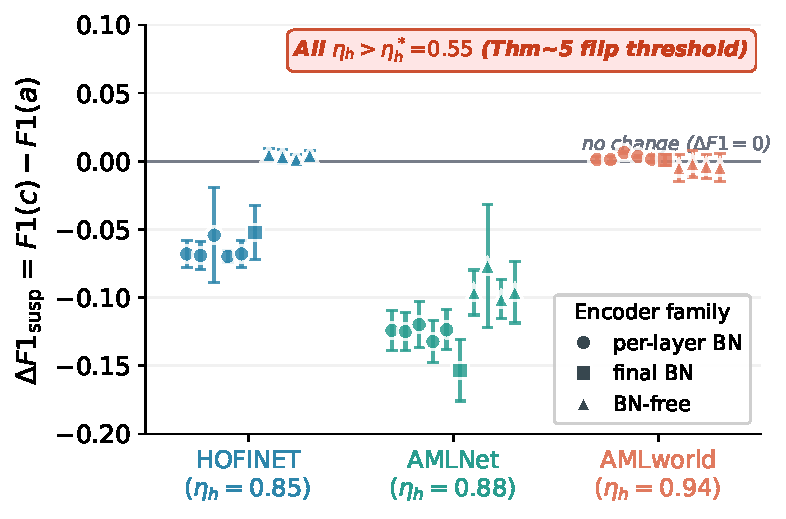
\includegraphics[width=\columnwidth]{figures/fig_theory_inset.pdf}
    \caption{Theory$\to$empirical bridge for Theorem~\ref{thm:meanpool}. X-axis: ego-neighborhood heterophily $\eta_h$; Y-axis: $F1_{\text{susp}}$ drop of setting (c) (transaction graph + subgraph pool) relative to (a) (transaction graph + augmentation, baseline). All three AML datasets lie above the mean-pool flip threshold $\eta_h^* = 0.55$ ($k{=}10$), and the markers report the observed $\Delta F1_{\text{susp}}$ for each encoder.}
    \label{fig:theory_inset}
\end{figure}

\subsection{Setting-level Performance Prediction}
\label{subsec:theory_pred}

\iffalse
$\eta_h^{\text{tx}} > 1/2 + 1/(2 \bar{d}_{\text{tx}})$이고($\bar{d}_{\text{tx}}$는 거래 그래프에서 중심 노드 주변 이웃의 평균 크기), 배치 정규화를 갖춘 인코더를 사용할 때, 위 분석은 $F1(b) \approx F1(d) > F1(a) > F1(c)$라는 경험적 패턴을 예측한다. 이는 동질성 회복과 평균 풀링의 신호 역전을 함께 고려한 예측이다. HOFINET에서는 배치 정규화를 갖춘 6개 인코더가 모두 이 순서를 따른다($\Delta(b{-}a) \in [+0.255, +0.405]$, $\Delta(c{-}a) \in [-0.070, -0.052]$).

요약하면, 정리~\ref{thm:knn_homophily}--\ref{thm:combined}은 행동 기반 k-NN view가 거래 간선의 낮은 동질성을 완화할 수 있는 조건을 다루며, 정리~\ref{thm:meanpool}와 명제~\ref{thm:hap}은 이웃 이질성이 높은 상황에서 풀링 방식이 신호 투영에 어떤 차이를 만드는지를 분석한다. 세 데이터셋(HOFINET, AMLworld, AMLNet)에 대한 정리~\ref{thm:combined}의 이상화된 하한과 평균 풀링 역전 임계값 $\eta_h^* = 0.55$($k{=}10$)의 경험적 비교는 부록~\ref{app:theory}의 Table~\ref{tab:theory_verify}에 제시된다. 또한 각 정리, 명제, 경험적 예측이 \method의 어느 설계 요소와 연결되는지는 부록~\ref{app:aux_tables}의 Table~\ref{tab:theorem_rq_map}에 정리된다.
\fi
When $\eta_h^{\text{tx}} > 1/2 + 1/(2 \bar{d}_{\text{tx}})$, where $\bar{d}_{\text{tx}}$ is the average ego-neighborhood size in the transaction graph, and the encoder uses batch normalization, the analysis above predicts the pattern $F1(b) \approx F1(d) > F1(a) > F1(c)$. The prediction combines view-level homophily recovery with mean-pool signal reversal. On HOFINET, all six BN-equipped encoders follow this ordering ($\Delta(b{-}a) \in [+0.255, +0.405]$, $\Delta(c{-}a) \in [-0.070, -0.052]$).

In summary, Theorems~\ref{thm:knn_homophily}--\ref{thm:combined} characterize the conditions under which a behavioral k-NN view can mitigate the low homophily of transaction edges, while Theorem~\ref{thm:meanpool} and Proposition~\ref{thm:hap} compare how different pooling choices affect the projected signal under high neighborhood heterophily. The empirical comparison between the idealized lower bound of Theorem~\ref{thm:combined} and the mean-pool flip threshold $\eta_h^* = 0.55$ at $k{=}10$ on HOFINET, AMLworld, and AMLNet is reported in Table~\ref{tab:theory_verify} of Appendix~\ref{app:theory}. The mapping from each theorem, proposition, and empirical prediction to the corresponding design element of \method is summarized in Table~\ref{tab:theorem_rq_map} of Appendix~\ref{app:aux_tables}.

\section{Experiments}
\label{sec:experiments}
\iffalse
본 실험의 목적은 \method 의 핵심 주장을 메커니즘 검증에서 시작하여 현실적인 운영 유효성 검증으로 확장하는 단계적 평가를 통해 검증하는 것이다. 우선, 행동 기반 k-NN 보조 view가 거래 그래프 내 의심 계좌 간의 직접적인 연결 부족 문제를 실제로 완화하고, view 수준의 동질성을 회복하는지 확인한다. 이는 이후 성능 향상의 전제가 되는 핵심 메커니즘을 검증하는 단계이다. 이어지는 분석에서는 회복된 view 위에서 서브그래프 풀링이 의심 신호를 추가로 증폭하는지, 그리고 이 효과가 인코더 정규화, 특히 BatchNorm에 어떻게 의존하는지를 분해하여 고찰한다. 이러한 메커니즘 및 구성 요소 분석을 바탕으로, 실제 AML 환경의 현실적 제약인 라벨 지연 및 cold-start 상황에서 최종 자기지도 표현이 지도학습 모델 대비 어느 정도의 실질적 경쟁력을 갖는지 평가한다. 마지막으로, 서로 다른 prevalence와 규모를 가진 AML 데이터셋에서도 동일한 메커니즘과 성능 경향이 재현되는지 검증함으로써 제안 방법론의 일반성을 확인한다. 이를 위해 본 연구에서는 다음 연구 질문을 중심으로 실험을 구성한다.
\fi
We evaluate \method through a staged study from mechanism to deployment. First, we ask whether the behavioral k-NN auxiliary view alleviates the lack of direct edges among suspicious accounts in the transaction graph and recovers view-level homophily, the mechanism underlying any subsequent gain. Second, we decompose whether subgraph pooling on the recovered view further amplifies the suspicious signal, and how this effect depends on encoder normalization, particularly BatchNorm. Third, we assess how competitive the resulting self-supervised representation is against supervised models under label delay and cold-start, the realistic constraints of AML operations. Fourth, we check whether the same mechanism and trends carry over to AML datasets with different prevalence and scale. The experiments are organized around the following research questions.

\begin{itemize}
    \item RQ1. \textbf{Effectiveness of behavioral k-NN view:} Does the behavioral k-NN auxiliary view alleviate the lack of direct edges among suspicious accounts in the transaction graph and recover view-level homophily?
    \item RQ2. \textbf{Subgraph aggregation and encoder stability:} Does subgraph pooling on the recovered view further amplify the suspicious signal, and how does this effect depend on encoder normalization, BatchNorm in particular?
    \item RQ3. \textbf{Self-supervised AML detection under label scarcity:} Does the self-supervised representation from \method remain competitive against supervised models under label delay and cold-start?
    \item RQ4. \textbf{Robustness across AML regimes:} Do the same mechanism and trends carry over to AML datasets with different prevalence and scale?
\end{itemize}

\subsection{Experimental Setting}

\iffalse
\textbf{Datasets.} 세 AML 데이터셋을 사용한다 (Table~\ref{tab:datasets}). 한국의 은행 간 이체 결제망인 HOFINET에서 발생한 실제 거래를 바탕으로 구축한 약 470만 건의 합성 데이터로, 가계 및 기업 타행 이체 40개월 (2021Q3--2024Q4) 분량의 패턴을 모델링한다.  NeurIPS 2023 공개 합성 벤치마크인 AMLworld~\cite{amlpatterns2024realistic}는 fan-out, scatter-gather, cycle 등 8가지 패턴을 모델링하며, 본 연구는 HI-Small (high illicit ratio, small size) 변형을 사용한다. High-prevalence regime 검증용 소규모 합성 벤치마크인 AMLNet~\cite{huda2025amlnet}은 AMLworld와 동일 피처 스키마를 공유한다.

\textbf{Account-level labels.} 세 데이터셋 모두 의심 거래 여부 라벨이 거래 transaction로 부여된다. 본 연구는 표준 graph-based AML and fraud detection 관행~\cite{dou2020enhancing,liu2021pick}을 따라 라벨을 account 수준으로 max-aggregate 한다. 즉, 한 번이라도 의심 거래의 출금 또는 입금 측에 관여한 계좌는 의심 (label$=1$), 그렇지 않은 계좌는 정상 (label$=0$) 으로 분류한다. 이 변환 후 의심 계좌 비율은 HOFINET 2.13\%, AMLworld 1.23\%, AMLNet 13.52\% 이다 (Table~\ref{tab:datasets}). 데이터셋 상세와 라벨 도출 의사코드는 부록~\ref{app:datasets} 에 수록한다.
\fi
\textbf{Datasets.} We use three AML datasets (Table~\ref{tab:datasets}). HOFINET contains roughly 4.7M synthetic transactions built from real activity on the Korean interbank settlement network, modeling 40 months of household and corporate inter-bank transfer patterns (2021Q3--2024Q4). AMLworld~\cite{amlpatterns2024realistic}, the NeurIPS 2023 open synthetic benchmark, models eight transaction patterns including fan-out, scatter-gather, and cycle; we use the HI-Small variant (high illicit ratio, small size). AMLNet~\cite{huda2025amlnet}, a small synthetic benchmark for the high-prevalence regime, shares the feature schema of AMLworld.

\textbf{Account-level labels.} All three datasets provide suspicious labels at the transaction level. Following standard graph-based AML and fraud detection practice~\cite{dou2020enhancing,liu2021pick}, we max-aggregate labels to the account level: an account is labeled suspicious (label$=1$) if it appeared on either side of at least one suspicious transaction, and normal (label$=0$) otherwise. The resulting suspicious-account ratios are 2.13\% (HOFINET), 1.23\% (AMLworld), and 13.52\% (AMLNet); see Table~\ref{tab:datasets}. Dataset details and label-derivation pseudocode are in Appendix~\ref{app:datasets}.

\begin{table}[h]
\centering
\caption{Dataset statistics. $\rho$ = suspicious account ratio.}
\label{tab:datasets}
\small
\setlength{\tabcolsep}{3pt}
\begin{tabular}{lrrrl}
\toprule
\textbf{Dataset} & $|V|$ & $|E|$ & $\rho$ & \textbf{Type} \\
\midrule
HOFINET           & 452{,}816 & 4{,}732{,}130 & 2.13\% & Synthetic (real-derived) \\
AMLworld          & 515{,}088 & 5{,}078{,}345 & 1.23\% & Synthetic (simulator) \\
AMLNet            &  11{,}000 & 1{,}090{,}172 & 13.52\% & Synthetic (simulator) \\
\bottomrule
\end{tabular}
\end{table}

\iffalse
\textbf{Ablation settings and encoders.} Table~\ref{tab:exp_design}은 본문 실험에서 사용하는 4가지 ablation setting과 10종 self-supervised encoder를 요약한다. 각 데이터셋에서 4개 setting과 10개 encoder의 Cartesian product를 평가하며, 공정 비교를 위해 모든 인코더에 동일한 BYOL-style bootstrap loss (Eq.~\eqref{eq:loss}) 와 하이퍼파라미터 (lr=5e-4, hidden=256, $L$=2, dropout=0.2, 200 ep) 를 적용한다.
\fi
\textbf{Ablation settings and encoders.} Table~\ref{tab:exp_design} summarizes the four ablation settings and ten self-supervised encoders used in the main experiments. We evaluate the Cartesian product of four settings and ten encoders on each dataset. For a fair comparison, all encoders use the same BYOL-style bootstrap loss (Eq.~\eqref{eq:loss}) and hyperparameters (lr=5e-4, hidden=256, $L$=2, dropout=0.2, 200 epochs).

\begin{table}[h]
\centering
\caption{Experimental design for self-supervised ablations. The four graph-view/contrastive-level settings are crossed with the ten encoders on each dataset.}
\label{tab:exp_design}
\small
\setlength{\tabcolsep}{3pt}
\resizebox{\columnwidth}{!}{%
\begin{tabular}{lp{0.22\columnwidth}p{0.38\columnwidth}L{0.26\columnwidth}}
\toprule
\textbf{Part} & \textbf{Option} & \textbf{\makecell[l]{Graph view \\/ BN regime}} & \textbf{\makecell[l]{Contrastive level \\/ encoders}} \\
\midrule
\multirowcell{4}[0pt][l]{\raisebox{-0.3ex}{Setting}}
                          & (a) baseline & Transaction graph & Node-level \\
                          & (b) RQ1 view & Behavioral k-NN view & Node-level \\
                          & (c) pooling-only & Transaction graph & Subgraph pool \\
                          & (d) proposed & Behavioral k-NN view & Subgraph pool \\
\midrule
\multirowcell{4}[0pt][l]{\raisebox{-8ex}{Encoder}}
                          & \multirowcell{2}[0pt][l]{\raisebox{-3ex}{Per-layer BN}} & \multirowcell{2}[0pt][l]{\raisebox{-3ex}{Layer-wise BN}} & GBT, DGI+BN, MVGRL+BN, \\
                          &                               &                                & GRACE+BN, GIN \\
                                                \cmidrule(l){2-4}
                          &  \multirowcell{1}[0pt][l]{\raisebox{0ex}{Final BN}}    & \multirowcell{1}[0pt][l]{\raisebox{0ex}{Output-only BN}} & BGRL \\
                                                \cmidrule(l){2-4}
                          &  \multirowcell{2}[0pt][l]{\raisebox{0ex}{BN-less}}     &   \multirowcell{2}[0pt][l]{\raisebox{0ex}{No BatchNorm}} & DGI, MVGRL, GRACE, GCA \\
\bottomrule
\end{tabular}}
\end{table}

\iffalse
\textbf{Supervised baselines.} Supervised baseline으로 generic GNN (GCN~\cite{kipf2016semi}, GAT~\cite{velivckovic2017graph}, GraphSAGE~\cite{hamilton2017inductive}), tabular (MLP, LightGBM~\cite{lightgbm2017}, XGBoost~\cite{xgboost2016}), 그리고 fraud- and anomaly-specific GNN (CARE-GNN~\cite{dou2020enhancing}, PC-GNN~\cite{liu2021pick}, BWGNN~\cite{tang2022rethinking}, GAGA~\cite{wang2023label}, ConsisGAD~\cite{chen2024consisgad}) 의 11종에 class-weight 보정을 적용한다. 세 데이터셋 모두 단일 관계 (계좌 간 이체) 의 동질 그래프이므로 fraud-specific GNN 들의 원 논문 multi-relation 구성 요소는 적용 불가하며, 단일 관계에서 작동하는 핵심 메커니즘만 활용한다 (Table~\ref{tab:rq3} 본문 참조).

\textbf{Evaluation protocol.} 평가 지표는 의심 클래스의 F1-score ($F1_{\text{susp}}$) 를 주 지표로, AUROC와 AUPRC를 보조 지표로 사용한다. 모든 실험은 10\%/10\%/80\% train/val/test 분할 (자기지도 인코더는 라벨 없이 학습하며 train 라벨은 downstream LogisticRegression에만 사용되므로 10\% 라벨로 충분하다; 시드별 동일 분할로 paired comparison을 보장) 과 4 시드 (2024--2027) 평균±표준편차로 보고한다. 통계적 유의성은 4-seed paired $t$-test로 검증하며 (Holm--Bonferroni 보정 적용, 상세 결과는 부록의 Table~\ref{tab:stat_test}), 시드별 원본 결과는 공개 리포지토리에 함께 배포한다.

\textbf{Downstream evaluation and implementation.} 자기지도 모델은 인코더를 고정하고 임베딩 $\mathbf{z}_i = [\mathbf{s}_i^{(1)} \| \mathbf{s}_i^{(2)}]$ 에 대해 LogisticRegression~\cite{pedregosa2011scikit} 으로 평가한다. 모든 실험은 Python 3.12 / PyTorch 2.10 / CUDA 12.8 / NVIDIA H100 80GB 환경에서 수행된다.
\fi
\textbf{Supervised baselines.} We apply class-weight correction to 11 supervised models: generic GNNs (GCN~\cite{kipf2016semi}, GAT~\cite{velivckovic2017graph}, GraphSAGE~\cite{hamilton2017inductive}), tabular methods (MLP, LightGBM~\cite{lightgbm2017}, XGBoost~\cite{xgboost2016}), and fraud- and anomaly-specific GNNs (CARE-GNN~\cite{dou2020enhancing}, PC-GNN~\cite{liu2021pick}, BWGNN~\cite{tang2022rethinking}, GAGA~\cite{wang2023label}, ConsisGAD~\cite{chen2024consisgad}). All three datasets are homogeneous single-relation graphs of account-to-account transfers, so the multi-relation components of the fraud-specific GNNs do not apply; we retain only their single-relation core mechanisms (see Section~\ref{subsec:rq3}).

\textbf{Evaluation protocol.} The primary metric is suspicious-class F1 ($F1_{\text{susp}}$); AUROC and AUPRC are secondary. We use a 10\%/10\%/80\% train/val/test split (self-supervised encoders learn without labels, and training labels are only used by the downstream LogisticRegression head, so 10\% is sufficient; the split is fixed per seed to enable paired comparison) and report mean$\pm$std over four seeds (2024--2027). Statistical significance is assessed by 4-seed paired $t$-test with Holm--Bonferroni correction (full results in Appendix Table~\ref{tab:stat_test}); seed-level raw results are released with the public repository.

\textbf{Downstream evaluation and implementation.} We evaluate self-supervised models by freezing the encoder and fitting LogisticRegression~\cite{pedregosa2011scikit} on the embedding $\mathbf{z}_i = [\mathbf{s}_i^{(1)} \| \mathbf{s}_i^{(2)}]$. All experiments run on Python 3.12 / PyTorch 2.10 / CUDA 12.8 / NVIDIA H100 80GB.

\subsection{Effectiveness and Mechanism of Behavioral k-NN View (RQ1)}\label{subsec:rq1}

\iffalse
RQ1은 행동 기반 k-NN view가 거래 그래프 내 의심 계좌 간 직접 연결 부족을 완화하고 view 수준의 동질성을 회복하는지를 정량적으로 검증한다.

\textbf{Quantitative gains across all 10 encoders.} 행동적 k-NN view는 baseline 대비 10종 인코더 모두에서 일관된 향상을 가져온다 (Table~\ref{tab:rq1}). BN-equipped 6 인코더는 +84\% $\sim$ +205\%, BN-less 4 인코더는 +24\% $\sim$ +29\% 의 개선을 보인다. 6 BN 인코더의 4-seed paired t-test는 Holm--Bonferroni 보정 후 모두 통계적으로 유의하다 (Table~\ref{tab:stat_test}; adjusted $p < 4 \times 10^{-5}$).
\fi
RQ1 quantitatively examines whether the behavioral k-NN view alleviates the lack of direct edges among suspicious accounts in the transaction graph and recovers view-level homophily.

\textbf{Quantitative gains across all 10 encoders.} The behavioral k-NN view yields a consistent gain over the baseline across all ten encoders (Table~\ref{tab:rq1}): +84\% to +205\% for the six BN-equipped encoders and +24\% to +29\% for the four BN-less encoders. On the six BN encoders, the 4-seed paired $t$-test is significant after Holm--Bonferroni correction (Table~\ref{tab:stat_test}; adjusted $p < 4 \times 10^{-5}$).

\begin{table}[H]
\centering
\caption{$F1_{\text{susp}}$ on HOFINET across all four ablation settings (10 encoders, 4-seed mean$\pm$std): transaction graph with node-level contrast, behavioral k-NN view with node-level contrast, transaction graph with subgraph pooling, and behavioral k-NN view with subgraph pooling (proposed). Best per row in bold, second-best underlined. $^{\dagger}$GIN uses per-layer BN inside its GINConv-based encoder.}
\label{tab:rq1}
\resizebox{\columnwidth}{!}{%
\begin{tabular}{lccccc}
\toprule
\textbf{Encoder} & \textbf{BN} & \makecell{\textbf{Tx graph}\\\textbf{node}} & \makecell{\textbf{k-NN view}\\\textbf{node}} & \makecell{\textbf{Tx graph}\\\textbf{pool}} & \makecell{\textbf{k-NN view}\\\textbf{pool}} \\
\midrule
GBT       & \multirow{4}{*}{Per-layer} & 0.266{\scriptsize±.010} & \underline{0.671}{\scriptsize±.003} & 0.197{\scriptsize±.002} & \textbf{0.673}{\scriptsize±.003} \\
DGI+BN    &            & 0.266{\scriptsize±.010} & \underline{0.670}{\scriptsize±.004} & 0.198{\scriptsize±.002} & \textbf{0.673}{\scriptsize±.002} \\
MVGRL+BN  &            & 0.266{\scriptsize±.010} & \underline{0.671}{\scriptsize±.004} & 0.198{\scriptsize±.002} & \textbf{0.673}{\scriptsize±.003} \\
GRACE+BN  &            & 0.286{\scriptsize±.004} & \underline{0.670}{\scriptsize±.004} & 0.216{\scriptsize±.002} & \textbf{0.673}{\scriptsize±.003} \\
\cmidrule{1-1}\cmidrule{3-6}
BGRL      & Final      & 0.306{\scriptsize±.012} & \underline{0.561}{\scriptsize±.008} & 0.253{\scriptsize±.016} & \textbf{0.639}{\scriptsize±.005} \\
GIN       & Per-layer$^{\dagger}$ & 0.181{\scriptsize±.035} & \underline{0.555}{\scriptsize±.038} & 0.127{\scriptsize±.001} & \textbf{0.578}{\scriptsize±.021} \\
\midrule
GCA       & \multirow{4}{*}{None} & 0.045{\scriptsize±.002} & \underline{0.058}{\scriptsize±.004} & 0.049{\scriptsize±.005} & \textbf{0.081}{\scriptsize±.011} \\
DGI       &            & 0.043{\scriptsize±.001} & \underline{0.054}{\scriptsize±.006} & 0.048{\scriptsize±.004} & \textbf{0.068}{\scriptsize±.004} \\
MVGRL     &            & 0.043{\scriptsize±.001} & \underline{0.055}{\scriptsize±.007} & 0.048{\scriptsize±.003} & \textbf{0.072}{\scriptsize±.008} \\
GRACE     &            & 0.044{\scriptsize±.001} & \underline{0.054}{\scriptsize±.005} & 0.045{\scriptsize±.003} & \textbf{0.070}{\scriptsize±.008} \\
\bottomrule
\end{tabular}}
\end{table}

\begin{table}[H]
\centering
\caption{S-S:S-B edge ratio and homophily by graph type across the three AML datasets. Best per dataset in bold, second-best underlined (higher Homophily and smaller S-S:S-B ratio are better). Behavioral k-NN consistently recovers homophily; structural k-NN (HOFINET only, ablation) does not.}
\label{tab:ss_sb}
\small
\setlength{\tabcolsep}{5pt}
\begin{tabular}{llcc}
\toprule
\textbf{Dataset} & \textbf{Graph} & \textbf{Homophily} & \textbf{S-S:S-B} \\
\midrule
\multirow{3}{*}{HOFINET}
  & Transaction      & 0.690 & \underline{1:5.7} \\
  & Structural k-NN  & \underline{0.965} & 1:9.7 \\
  & Behavioral k-NN  & \textbf{0.981} & \textbf{1:1.4} \\
\midrule
\multirow{2}{*}{AMLworld}
  & Transaction      & \underline{0.886} & \underline{1:15.8} \\
  & Behavioral k-NN  & \textbf{0.980} & \textbf{1:9.4} \\
\midrule
\multirow{2}{*}{AMLNet}
  & Transaction      & \underline{0.791} & \underline{1:7.2} \\
  & Behavioral k-NN  & \textbf{0.900} & \textbf{1:1.3} \\
\bottomrule
\end{tabular}
\end{table}

\iffalse
\textbf{Homophily recovery via behavioral similarity.} 메커니즘 측면에서 거래 그래프의 S-S:S-B = 1:5.7 (Table~\ref{tab:ss_sb}) 에서 행동적 k-NN 그래프는 1:1.4로 개선되며 (Figure~\ref{fig:intro_homophily}), 동질성도 0.690 → 0.981로 상승한다 (동질성 $h$ 는 전체 엣지 중 양 끝 노드 라벨이 같은 비율(=edge homophily)로 정의한다). 자금세탁 계좌들이 분할 거래와 다단계 이체로 유사한 거래 패턴을 공유하므로 행동적 유사도 기반 k-NN이 자연스럽게 의심 계좌끼리 연결한다. 반면, 구조적 k-NN은 1:9.7로 오히려 악화되는데, 이는 degree와 centrality가 의심 여부보다는 네트워크 위치를 반영하기 때문이다.

\textbf{Robustness to $k$.} GBT에서 $k \in \{5, 10, 20, 50\}$을 측정한 결과 $k=10$이 최적이며, $k=5$ 에서도 (d) $F1_{\text{susp}}$ $= 0.676$ 으로 안정적이다 (상세는 부록의 Table~\ref{tab:k_sens}). $k > 10$ 에서는 benign 혼입으로 S-S 밀도가 희석되어 단조 하락하며 ($k{=}50$: 0.661), 전체 범위에서 (d) $F1_{\text{susp}}$ 의 편차가 0.021 이내로 $k$ 에 강건하다.
\fi
\textbf{Homophily recovery via behavioral similarity.} Mechanistically, the transaction graph's S-S:S-B of 1:5.7 (Table~\ref{tab:ss_sb}) improves to 1:1.4 under the behavioral k-NN graph (Figure~\ref{fig:intro_homophily}), and homophily rises from 0.690 to 0.981 (we define homophily $h$ as the fraction of edges whose endpoints share the same label, i.e., edge homophily). Money-laundering accounts often share similar transaction patterns through split transfers and multi-hop routing, so behavioral-similarity k-NN tends to link suspicious accounts together. The structural k-NN, in contrast, worsens to 1:9.7: degree and centrality reflect network position rather than suspicious behavior.

\textbf{Robustness to $k$.} Across $k \in \{5, 10, 20, 50\}$ on GBT, $k=10$ is optimal, and $k=5$ also remains stable at (d) $F1_{\text{susp}} = 0.676$ (Appendix Table~\ref{tab:k_sens}). Beyond $k > 10$, benign mixing dilutes S-S density and (d) drops monotonically ($k{=}50$: 0.661); the spread of (d) $F1_{\text{susp}}$ over the whole range stays within 0.021, suggesting robustness to $k$.

\subsection{Subgraph Aggregation and Encoder Stability (RQ2)}
\label{subsec:rq2}

\iffalse
RQ1이 행동 기반 k-NN view의 동질성 회복 여부를 검증했다면, RQ2는 회복된 view 위에서 서브그래프 단위 집계가 실제로 의심 신호를 증폭하는지, 그리고 그 효과가 인코더 정규화에 어떻게 의존하는지를 분해한다. 핵심 결과는 명확하다. 서브그래프 풀링은 독립적으로 항상 좋은 모듈이 아니라, view가 충분히 동질적이고 인코더가 과도하게 포화되지 않았을 때 작동하는 조건부 증폭기이다.
\fi
RQ1 verified the homophily recovery of the behavioral k-NN view; RQ2 now decomposes whether subgraph-level aggregation on the recovered view actually amplifies the suspicious signal, and how this effect depends on encoder normalization. The takeaway is direct: subgraph pooling is not a uniformly positive module on its own, but a conditional amplifier that works when the view is sufficiently homophilic and the encoder is not over-saturated.


\begin{figure}[H]
    \centering
    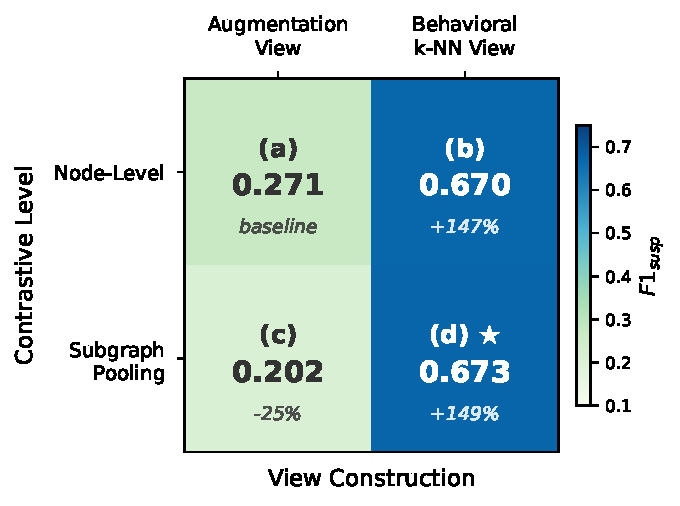
\includegraphics[width=0.85\columnwidth]{figures/fig_rq2_ablation.pdf}
    \caption{$F1_{\text{susp}}$ across the four ablation settings of the two design axes (graph view $\times$ contrastive level) on HOFINET, averaged over 4 per-layer BN encoders (GBT, DGI+BN, MVGRL+BN, GRACE+BN). Settings: (a) tx-view+node, (b) k-NN-view+node, (c) tx-view+pool, (d) k-NN-view+pool (proposed). The behavioral k-NN view is the primary driver, and subgraph pooling provides additional gains only when combined with it.}
    \label{fig:rq2_ablation}
\end{figure}

\begin{table*}[h]
\centering
\caption{BatchNorm architectural ablation summary at setting (d) on HOFINET (4-seed paired $t$-test, Holm-Bonferroni adjusted; \# = pairs within family). BN presence is dominant; BN position and convolution type are secondary. Per-pair statistics in Table~\ref{tab:stat_test}.}
\label{tab:bn_summary}
\begin{tabular}{llccc}
\toprule
\textbf{Axis} & \textbf{Better $>$ Worse (mean $F1_{\text{susp}}$)} & $\boldsymbol{\Delta F1_{\text{susp}}}$ & \textbf{\# pairs} & $\boldsymbol{\max p_{\text{adj}}}$ \\
\midrule
(i) BN presence  & \{DGI, MVGRL, GRACE\}+BN (0.673) $>$ no-BN (0.070)            & 0.602 & 3 & $1.21\times 10^{-6}$ \\
(ii) BN position & Per-layer 4 enc.\ (0.673) $>$ Final-only BGRL (0.639)          & 0.034 & 4 & $5.55\times 10^{-3}$ \\
(iii) Conv type  & GCNConv 4 enc.\ (0.673) $>$ GINConv GIN (0.578)                & 0.095 & 4 & $1.25\times 10^{-2}$ \\
\bottomrule
\end{tabular}
\end{table*}
\iffalse
\textbf{Conditional amplification across the 4-setting ablation.} 서브그래프 풀링의 효과는 결합되는 view와 인코더의 정규화 깊이에 동시에 의존한다 (Figure~\ref{fig:rq2_ablation}). HOFINET에서 (d) 의 (b) 대비 개선 폭은 정규화 깊이에 반비례하며, per-layer BN 4종은 +0.002 $\sim$ +0.003의 미미한 차이를 보이는 반면, BGRL은 +0.078, BN 미포함 인코더는 평균 +0.018의 개선을 보인다. 거래 그래프에 풀링만 적용한 (c)는 BN-augmented 인코더에서 (a) 대비 $-$17\% $\sim$ $-$30\% 저하한다 (Figure~\ref{fig:rq2_ablation} 의 (c) 막대 참조; 6 BN 인코더 측정 $-17.1\%$ (BGRL) $\sim$ $-29.9\%$ (GIN)). 이는 Section~\ref{subsec:subgraph_pool} 의 noise amplification 메커니즘 (정리~\ref{thm:meanpool}) 과 일치한다.

관찰된 4-setting 패턴 (b)$>$(a)$>$(c), (d)$\approx$(b) 는 정리~\ref{thm:knn_homophily}, \ref{thm:meanpool} 과 앞선 경험적 예측과 일치한다. (b)$\to$(d) 개선의 paired t-test는 GBT $p=1.83{\times}10^{-3}$, BGRL Holm-보정 $p=2.66{\times}10^{-4}$ 로 유의하다 (Table~\ref{tab:stat_test}). AMLworld 의 per-layer BN 인코더는 (i) 1.23\% 의 낮은 prevalence 로 인해 $F1_{\text{susp}}$ 절대 스케일이 작고(prevalence floor) (ii) per-layer BN 으로 표현이 빠르게 포화(BN-rich saturation)되기 때문에, (b)$>$(d) 의 미세 역전이 관찰된다 ($-$0.0014 $\sim$ $-$0.0016, Table~\ref{tab:rq4}).

이는 서브그래프 풀링이 conditional amplifier로서 (i) 각 view의 class homophily와 (ii) 인코더 정규화 깊이 두 조건에 의존함을 보인다. \method 의 (d) 설정은 두 조건 모두에서 강건하다.
\fi
\textbf{Conditional amplification across the 4-setting ablation.} The effect of subgraph pooling depends jointly on the paired view and the encoder's normalization depth (Figure~\ref{fig:rq2_ablation}). On HOFINET, the (d)-over-(b) gain is inversely related to normalization depth: the four per-layer BN encoders show a marginal +0.002 to +0.003, BGRL gains +0.078, and the BN-less encoders gain +0.018 on average. Setting (c), pooling on the transaction graph alone, degrades by $-$17\% to $-$30\% from (a) across BN-augmented encoders (see the (c) bars in Figure~\ref{fig:rq2_ablation}; measured $-17.1\%$ for BGRL to $-29.9\%$ for GIN across six BN encoders). This is consistent with the noise-amplification mechanism in Section~\ref{subsec:subgraph_pool} (Theorem~\ref{thm:meanpool}).

The observed 4-setting pattern (b)$>$(a)$>$(c), (d)$\approx$(b) aligns with Theorems~\ref{thm:knn_homophily} and \ref{thm:meanpool} and our earlier empirical predictions. The (b)$\to$(d) gain is significant under paired $t$-tests (GBT $p=1.83{\times}10^{-3}$, BGRL Holm-adjusted $p=2.66{\times}10^{-4}$; Table~\ref{tab:stat_test}). On AMLworld, the per-layer BN encoders show a slight (b)$>$(d) reversal ($-$0.0014 to $-$0.0016, Table~\ref{tab:rq4}), attributable to (i) a low absolute $F1_{\text{susp}}$ scale under 1.23\% prevalence (prevalence floor) and (ii) rapid representational saturation from per-layer BN (BN-rich saturation).

Subgraph pooling thus acts as a conditional amplifier whose effect depends on (i) each view's class homophily and (ii) encoder normalization depth. The (d) setting of \method remains robust under both conditions.

\iffalse
\textbf{BatchNorm as the dominant architectural axis.} BatchNorm (BN) 유무는 이 조건부 효과를 해석하는 핵심 축이다 (Figure~\ref{fig:rq2_bn}, 10종 인코더에 대한 설정 (a) 와 (d) 의 $F1_{\text{susp}}$ 비교). 설정 (d) 의 4-seed paired $t$-test (Holm-보정) 결과를 Table~\ref{tab:bn_summary} 에 요약한다 (쌍별 통계는 Table~\ref{tab:stat_test}). (i) BN 유무가 지배적이며 ($\Delta F1_{\text{susp}} \approx 0.60$, 약 10배 격차), 동일 아키텍처 통제 비교 3쌍에서 격차가 BN 자체에 기인함이 확인된다. (ii) BN 위치 (per-layer $\succ$ final-only) 와 (iii) convolution 종류 (GCNConv $\succ$ GINConv) 도 유의하나, 효과 크기는 (i) 의 1/18 $\sim$ 1/6 수준으로 보조적이다. Per-layer BN 인코더 4종 (GBT, DGI+BN, MVGRL+BN, GRACE+BN) 은 원래 서로 다른 contrastive paradigm (BarlowTwins, JSD, BootstrapLatent, InfoNCE) 에서 유래하나 동일 BYOL bootstrap loss 하에서 모두 0.673 $\sim$ 0.674로 수렴하므로, BN이 보장되면 paradigm 차이는 무시 가능하다.
\fi
\textbf{BatchNorm as the dominant architectural axis.} The presence of BatchNorm (BN) is the central axis for interpreting this conditional effect (Figure~\ref{fig:rq2_bn}, comparing $F1_{\text{susp}}$ at settings (a) and (d) across ten encoders). Table~\ref{tab:bn_summary} summarizes the setting-(d) 4-seed paired $t$-tests with Holm correction (per-pair statistics in Table~\ref{tab:stat_test}). (i) BN presence dominates ($\Delta F1_{\text{susp}} \approx 0.60$, roughly a 10$\times$ gap), and three controlled comparisons (same architecture, BN as the only difference) confirm that the gap is attributable to BN itself. (ii) BN position (per-layer $\succ$ final-only) and (iii) convolution type (GCNConv $\succ$ GINConv) are also significant but secondary, with effect sizes about 1/18 to 1/6 of (i). The four per-layer BN encoders (GBT, DGI+BN, MVGRL+BN, GRACE+BN) originate from different contrastive paradigms (BarlowTwins, JSD, BootstrapLatent, InfoNCE), yet under the same BYOL bootstrap loss they all converge to 0.673--0.674, suggesting that once BN is in place the paradigm difference is negligible.

\begin{figure}[h]
    \centering
    \begin{subfigure}{0.49\columnwidth}
        \centering
        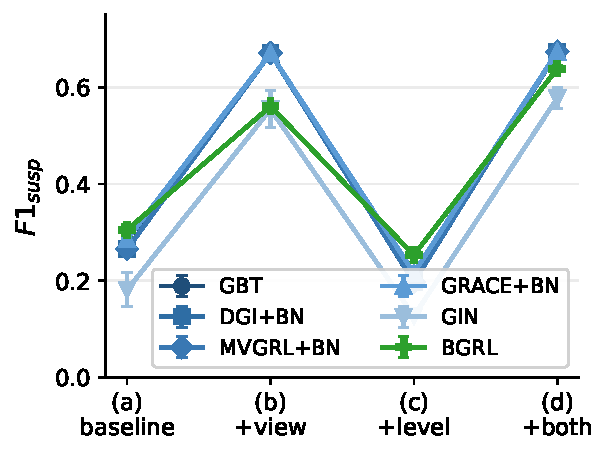
\includegraphics[width=\linewidth]{figures/fig_rq3_bn_a.pdf}
        \caption{BN-augmented encoders}
        \label{fig:rq2_bn_a}
    \end{subfigure}
    \hfill
    \begin{subfigure}{0.49\columnwidth}
        \centering
        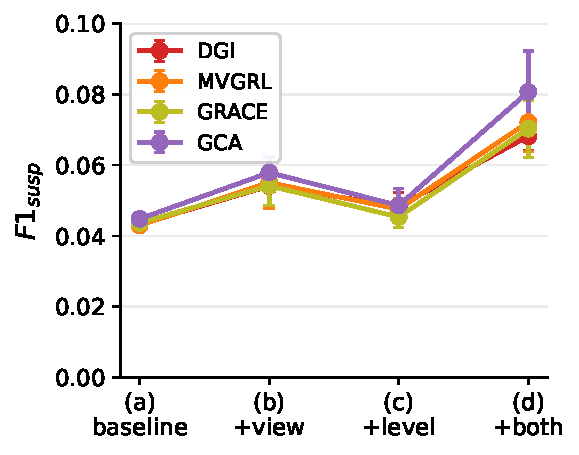
\includegraphics[width=\linewidth]{figures/fig_rq3_bn_b.pdf}
        \caption{BN-free encoders}
        \label{fig:rq2_bn_b}
    \end{subfigure}
    \caption{$F1_{\text{susp}}$ trajectory across four ablation settings (a)/(b)/(c)/(d) for 10 encoders (HOFINET, 4-seed mean$\pm$std). Note the different y-axis scales. (a) Per-layer BN family (GBT, DGI+BN, MVGRL+BN, GRACE+BN, GIN) saturates at the (b) view-only step; final-only BN (BGRL) shows strong (b)$\to$(d) amplification. (b) BN-free encoders (DGI, MVGRL, GRACE, GCA) collapse to random level ( $\sim$ 0.04--0.08), confirming the structural collapse implied by Theorem~\ref{thm:bn_collapse}. BatchNorm is the dominant architectural factor; subgraph pooling provides complementary amplification only for under-normalized encoders.}
    \label{fig:rq2_bn}
\end{figure}

\iffalse
\begin{theorem}[BN-conditional collapse]
BYOL-style bootstrap loss~\eqref{eq:loss} 하에서, 인코더 $f_\theta$ 의 trivial constant solution $f_\theta(\cdot) \equiv c$ 는 $f_\theta$ 가 BN layer 를 포함하지 않을 때에만 $\mathcal{L} = 0$ 의 attainable global minimum 이다. 적어도 하나의 BN layer 를 포함하는 인코더는 batch normalization 의 정의에 의해 trivial constant solution 을 차단한다.
\end{theorem}
\fi
\begin{theorem}[BN-conditional collapse]\label{thm:bn_collapse}
Under the BYOL-style bootstrap loss~\eqref{eq:loss}, the trivial constant solution $f_\theta(\cdot) \equiv c$ of an encoder $f_\theta$ is an attainable global minimum at $\mathcal{L} = 0$ only when $f_\theta$ contains no BN layer. An encoder with at least one BN layer blocks the trivial constant solution by the definition of batch normalization.
\end{theorem}

\iffalse
\textbf{Empirical confirmation of BN-conditional collapse.} 설정 (a) 의 BN-less 인코더 $F1_{\text{susp}}$ $\approx 0.04$ 가 HOFINET random-classifier upper bound $2\rho/(1+\rho) \approx 0.042$(양성 비율 $\rho$로 무작위 예측할 때 기대 가능한 $F1_{\text{susp}}$의 상한)과 일치하여 collapse가 구조적으로 발생함을 직접 확인한다 (정리~\ref{thm:bn_collapse} 의 형식 증명은 부록~\ref{app:bn_proof}). 이 collapse의 실질적 영향은 prevalence에 의존한다: low prevalence ($\rho \leq 2\%$) 에서는 random-classifier 상한 자체가 0.04로 낮아 collapse가 치명적이나, AMLNet ($\rho = 13.52\%$) 에서는 BN-less DGI도 $F1_{\text{susp}} \approx 0.40$을 달성하여 (Section~\ref{subsec:rq4}) collapse의 절대 영향이 완화된다. 따라서 RQ2는 단순한 pooling ablation이 아니라, \method 의 성능이 ``동질성 회복된 view + 적절한 정규화 + 조건부 subgraph amplification''의 결합에서 발생함을 확인한다.
\fi
\textbf{Empirical confirmation of BN-conditional collapse.} At setting (a), the BN-less encoders sit at $F1_{\text{susp}} \approx 0.04$, matching the HOFINET random-classifier upper bound $2\rho/(1+\rho) \approx 0.042$ (the maximum $F1_{\text{susp}}$ attainable by random prediction at positive rate $\rho$). This directly confirms that the collapse occurs structurally; the formal proof of Theorem~\ref{thm:bn_collapse} is in Appendix~\ref{app:bn_proof}. The practical impact of this collapse depends on prevalence: at low prevalence ($\rho \leq 2\%$) the random-classifier bound is itself only about 0.04, so collapse is fatal; on AMLNet ($\rho = 13.52\%$), BN-less DGI reaches $F1_{\text{susp}} \approx 0.40$ (Section~\ref{subsec:rq4}), so the absolute impact is muted. RQ2 therefore suggests that the gain of \method comes not from a single pooling ablation but from the combination of homophily-recovered view, appropriate normalization, and conditional subgraph amplification.

\subsection{Self-Supervised Detection under Label Scarcity (RQ3)}
\label{subsec:rq3}

\iffalse
앞선 두 질문이 \method 내부의 메커니즘과 구성요소를 검증했다면, RQ3는 그 결과물이 실제 AML 제약, 즉 라벨 지연과 cold-start 상황에서 지도학습 모델 대비 경쟁력 있는지를 평가한다. 이 비교에서 \method 는 representation 학습 단계에서 라벨을 사용하지 않으며, downstream 평가에서만 동일한 10\% train label을 LogisticRegression head에 사용한다.
\fi
The previous two questions verified the internal mechanism and components of \method; RQ3 now asks whether the resulting representation is competitive with supervised models under realistic AML constraints, label delay and cold-start. In this comparison \method uses no labels during representation learning; the same 10\% training labels are used only by the downstream LogisticRegression head.

\begin{figure*}[t!]
\centering
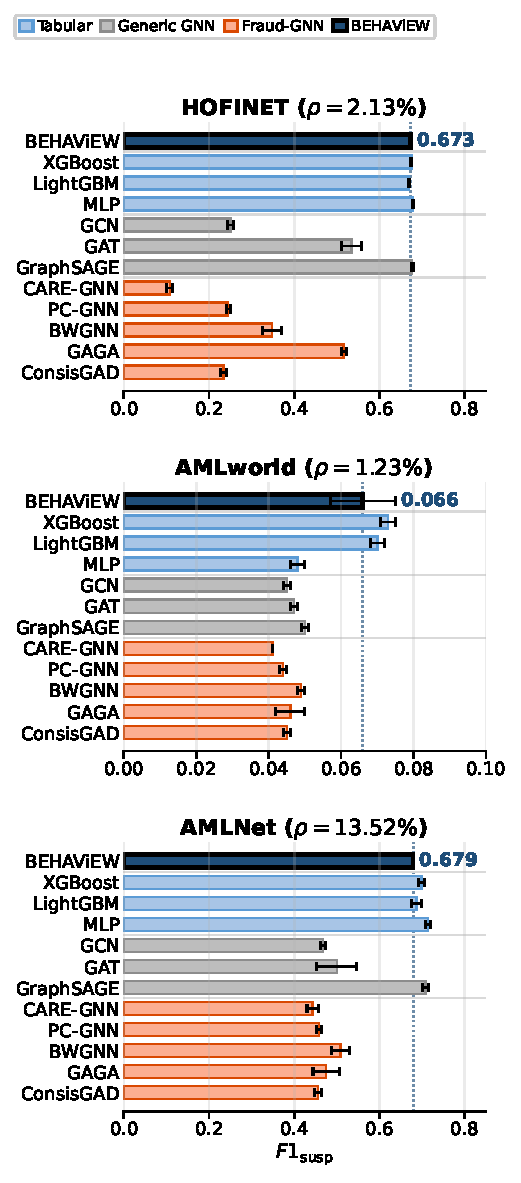
\includegraphics[width=0.98\textwidth]{figures/fig_rq3_baseline.pdf}
\caption{Self-supervised \method (rightmost dark-blue bar) vs.\ 11 supervised baselines across three AML datasets (4-seed mean$\pm$std on the 80\% holdout). Dotted horizontal line marks \method 's $F1_{\mathrm{susp}}$ for visual comparison. The five fraud-specific GNNs spanning CIKM'20--ICLR'24 (CARE-GNN, PC-GNN, BWGNN, GAGA, ConsisGAD) all underperform \method on HOFINET by $-0.16$ to $-0.57$ in $F1_{\mathrm{susp}}$ despite using ground-truth labels. Per-panel y-axis scales differ to accommodate dataset-specific suspicious prevalence ($\rho$); per-metric values including AUROC and AUPRC are reported in Appendix Table~\ref{tab:rq3}.}
\label{fig:rq3_baseline}
\end{figure*}

\iffalse
\textbf{Self-supervised parity with supervised baselines.} Figure~\ref{fig:rq3_baseline} 는 세 데이터셋에서 \method (제안 설정 (d), 데이터셋별 최강 인코더) 와 11종 지도학습 baseline 의 $F1_{\text{susp}}$ 를 비교한다: 3 tabular (XGBoost, LightGBM, MLP), 3 generic GNN (GCN, GAT, GraphSAGE), 5 fraud-specific GNN (CARE-GNN~\cite{dou2020enhancing}, PC-GNN~\cite{liu2021pick}, BWGNN~\cite{tang2022rethinking}, GAGA~\cite{wang2023label}, ConsisGAD~\cite{chen2024consisgad}; AUROC/AUPRC 전체 수치는 Appendix Table~\ref{tab:rq3}). Fraud-specific GNN baseline 은 세 데이터셋이 모두 homogeneous single-relation 거래 그래프이므로 각 방법의 핵심 메커니즘만 적용한다 (CARE-GNN: similarity-weighted aggregation; PC-GNN: label-distribution-aware edge sampling; BWGNN: multi-band spectral filters; GAGA: label-group separated aggregation; ConsisGAD: multi-view consistency).

\method 의 dark-blue 막대는 세 데이터셋 모두에서 supervised 상위 cluster 내에 자리한다 (Figure~\ref{fig:rq3_baseline} 의 점선 reference line). HOFINET 과 AMLNet 에서는 best supervised baseline (MLP) 과 시각적으로 거의 구분되지 않는 수준 (gap 0.006 / 0.035) 이며, AMLworld 에서는 tree-based 가 약간 앞서나 \method 가 GNN 지도학습 8종 (generic + fraud-specific) 을 모두 상회한다. 라벨 신호 없이 학습한 자기지도 표현이 라벨을 직접 활용한 supervised 설계와 동등하거나 그 이상의 capacity 를 확보함을 시각적으로 확인할 수 있다.
\fi
\textbf{Self-supervised parity with supervised baselines.} Figure~\ref{fig:rq3_baseline} compares $F1_{\text{susp}}$ between \method (the proposed (d) setting with the strongest encoder per dataset) and 11 supervised baselines across the three datasets: 3 tabular (XGBoost, LightGBM, MLP), 3 generic GNN (GCN, GAT, GraphSAGE), and 5 fraud-specific GNN (CARE-GNN~\cite{dou2020enhancing}, PC-GNN~\cite{liu2021pick}, BWGNN~\cite{tang2022rethinking}, GAGA~\cite{wang2023label}, ConsisGAD~\cite{chen2024consisgad}; full AUROC/AUPRC numbers are in Appendix Table~\ref{tab:rq3}). All three datasets are homogeneous single-relation transaction graphs, so the fraud-specific GNN baselines retain only their core single-relation mechanisms (CARE-GNN: similarity-weighted aggregation; PC-GNN: label-distribution-aware edge sampling; BWGNN: multi-band spectral filters; GAGA: label-group separated aggregation; ConsisGAD: multi-view consistency).

The dark-blue bar of \method sits within the upper supervised cluster on all three datasets (dotted reference line in Figure~\ref{fig:rq3_baseline}). On HOFINET and AMLNet it is visually almost indistinguishable from the best supervised baseline (MLP), with gaps of 0.006 and 0.035 respectively. On AMLworld, tree-based methods are slightly ahead, but \method exceeds all eight GNN-supervised models (generic and fraud-specific). The figure suggests that a self-supervised representation learned without label signal can match or exceed the capacity of supervised designs that use labels directly.

\iffalse
\textbf{Robustness under cold-start label scarcity.} \method 의 라벨 의존도가 LR head 한 개에 국한되므로, 라벨이 1\% 로 감소하는 cold-start 환경 (Table~\ref{tab:label_fraction}) 에서도 $F1_{\text{susp}} = 0.654$ 의 robust 한 성능을 유지하는 반면, supervised 모델은 동일 환경에서 학습 자체가 불안정해진다. 실제 AML 운영에서의 6개월 라벨 지연과 0.5\% $\sim$ 2\% 의심 비율을 반영한 환경에서는 \method 만 학습 가능한 유일한 옵션이다. 지도학습 대비 격차가 prevalence와 함께 좁아지는 점 (HOFINET 0.006, AMLNet 0.035) 과 AMLworld (1.23\% prevalence, 실제 AML 에 가장 근접) 에서 모든 GNN supervised 를 상회하는 점은, \method 의 가치가 라벨 부족 + 저 prevalence regime 에 집중되어 있음을 시사한다.

\textbf{Underperformance of fraud-specific GNNs.} Fraud- and anomaly-specific GNN들은 CIKM 2020부터 ICLR 2024까지의 SOTA 진화 (CARE-GNN $\to$ PC-GNN $\to$ BWGNN $\to$ GAGA $\to$ ConsisGAD) 전 구간에서 \method 미만에 머문다 (HOFINET 최고 GAGA 0.516 vs \method 0.673, $-$0.16). 다섯 모델 모두 message passing 수준에서 fraud heterogeneity를 다루지만 거래 그래프의 graph-level anti-homophily (S-S:S-B $=$ 1:5.7 $\sim$ 1:15.8) 자체는 변경하지 않기 때문으로 해석된다. ConsisGAD의 multi-view consistency 또한 동일 그래프에서 view를 변형하므로 그래프 수준 동질성 결함을 그대로 보존한다. \method 은 이와 직교하는 접근으로 거래 그래프와 구조적으로 독립된 행동적 k-NN view를 도입하여 동일 결함을 graph 수준에서 해소한다.

\textbf{Operational utility under limited analyst budget.} \method GBT의 HOFINET precision@$k$ ($k \in \{50, 100, 200, 400, 800\}$, 4 seed) 는 0.875, 0.853, 0.834, 0.791, 0.746으로, 상위 400건 예산에서 약 317건의 진성 의심 계좌를 검출한다.
\fi
\textbf{Robustness under cold-start label scarcity.} Because the label dependence of \method is confined to a single LR head, it maintains a robust $F1_{\text{susp}} = 0.654$ in the cold-start regime where labels drop to 1\% (Table~\ref{tab:label_fraction}); supervised models become unstable to train under the same regime. In an operational AML setting with six-month label delay and a 0.5\%--2\% suspicious rate, \method is the only trainable option among the methods compared. The gap to supervised models narrows with prevalence (HOFINET 0.006, AMLNet 0.035), and \method outperforms all GNN-supervised baselines on AMLworld (1.23\% prevalence, closest to real AML); together these suggest that the value of \method concentrates in the label-scarce, low-prevalence regime.

\textbf{Underperformance of fraud-specific GNNs.} Fraud- and anomaly-specific GNNs stay below \method across the full CIKM 2020 to ICLR 2024 SOTA evolution (CARE-GNN $\to$ PC-GNN $\to$ BWGNN $\to$ GAGA $\to$ ConsisGAD); on HOFINET, the strongest of these (GAGA 0.516) falls $-0.16$ short of \method (0.673). All five address fraud heterogeneity at the message-passing level but leave the graph-level anti-homophily of the transaction graph (S-S:S-B $=$ 1:5.7 to 1:15.8) unchanged. ConsisGAD's multi-view consistency also operates on views of the same graph, so the graph-level homophily defect persists. \method takes an orthogonal route: it introduces a behavioral k-NN view that is structurally independent of the transaction graph, resolving the defect at the graph level.

\textbf{Operational utility under limited analyst budget.} \method with GBT reaches HOFINET precision@$k$ of 0.875, 0.853, 0.834, 0.791, and 0.746 for $k \in \{50, 100, 200, 400, 800\}$ (4 seeds), detecting about 317 true suspicious accounts within a top-400 budget.

\subsection{Robustness Across AML Regimes (RQ4)}\label{subsec:rq4}

마지막으로 RQ4는 앞선 RQ1--RQ3의 패턴이 HOFINET에만 특화된 결과인지, 아니면 prevalence와 규모가 다른 AML regime에서도 재현되는지를 확인한다. 이를 위해 HOFINET과 구조적 특성이 상이한 두 데이터셋 (AMLworld: 대규모 합성, $\rho{=}1.23\%$; AMLNet: 소규모 합성, $\rho{=}13.52\%$) 에서 동일한 4-setting ablation을 반복하였다. Table~\ref{tab:rq4}는 5종 인코더에 대한 4가지 설정의 $F1_{\text{susp}}$를 보여준다.

\begin{table}[h]
\centering
\caption{RQ4: Results on AMLworld ($\rho{=}1.23\%$) and AMLNet ($\rho{=}13.52\%$) ($F1_{\text{susp}}$, 4-seed mean$\pm$std). Behavioral k-NN view (b, d) consistently outperforms baselines (a, c) across both datasets.}
\label{tab:rq4}
\resizebox{\columnwidth}{!}{%
\begin{tabular}{lccccc}
\toprule
 & & \multicolumn{2}{c}{\textbf{Node-level}} & \multicolumn{2}{c}{\textbf{Subgraph Pooling}} \\
\cmidrule(lr){3-4} \cmidrule(lr){5-6}
\textbf{Encoder} & \textbf{BN} & \textbf{(a) Aug.} & \textbf{(b) k-NN} & \textbf{(c) Aug.} & \textbf{(d) k-NN} \\
\midrule
\multicolumn{6}{l}{\textit{AMLworld (N=515K, $\rho$=1.23\%)}} \\
\midrule
BGRL      & \checkmark & 0.038{\scriptsize±.003} & \underline{0.061}{\scriptsize±.003} & 0.039{\scriptsize±.002} & 0.066{\scriptsize±.007} \\
GBT       & \checkmark & 0.042{\scriptsize±.002} & 0.049{\scriptsize±.001} & 0.043{\scriptsize±.001} & \underline{0.047}{\scriptsize±.001} \\
DGI+BN    & \checkmark & 0.042{\scriptsize±.002} & 0.049{\scriptsize±.001} & 0.044{\scriptsize±.001} & \underline{0.048}{\scriptsize±.001} \\
GRACE+BN  & \checkmark & 0.041{\scriptsize±.001} & \underline{0.048}{\scriptsize±.001} & 0.044{\scriptsize±.000} & 0.055{\scriptsize±.002} \\
DGI       &            & 0.038{\scriptsize±.007} & \underline{0.049}{\scriptsize±.004} & 0.033{\scriptsize±.005} & 0.052{\scriptsize±.005} \\
\midrule
\multicolumn{6}{l}{\textit{AMLNet (N=11K, $\rho$=13.52\%)}} \\
\midrule
BGRL      & \checkmark & 0.448{\scriptsize±.018} & \underline{0.668}{\scriptsize±.013} & 0.295{\scriptsize±.013} & 0.679{\scriptsize±.005} \\
GBT       & \checkmark & 0.426{\scriptsize±.011} & \underline{0.669}{\scriptsize±.012} & 0.302{\scriptsize±.009} & 0.679{\scriptsize±.002} \\
DGI+BN    & \checkmark & 0.426{\scriptsize±.011} & \underline{0.672}{\scriptsize±.014} & 0.302{\scriptsize±.010} & 0.679{\scriptsize±.001} \\
GRACE+BN  & \checkmark & 0.431{\scriptsize±.014} & \underline{0.673}{\scriptsize±.010} & 0.299{\scriptsize±.006} & 0.678{\scriptsize±.004} \\
DGI       &            & 0.397{\scriptsize±.015} & \underline{0.593}{\scriptsize±.014} & 0.301{\scriptsize±.007} & 0.608{\scriptsize±.017} \\
\bottomrule
\end{tabular}}
\end{table}

AMLworld와 AMLNet 모두에서 행동적 k-NN view의 효과가 재현된다.

\textbf{AMLworld: replication with BN-rich saturation.} AMLworld의 BGRL 인코더 기준 설정 (d)에서 $F1_{\text{susp}}$ 0.066을 달성하여 baseline (a) 대비 +73\%의 상대적 개선을 보이며, (b) $>$ (a) 패턴은 모든 인코더에서 일관된다. 다만 서브그래프 풀링의 추가 효과는 BN-rich 인코더에서 marginal하거나 음의 방향으로 나타나는데, GBT와 DGI+BN에서 (b) 대비 (d)가 $-$0.0014 $\sim$ $-$0.0016 F1로 통계적으로 약간 저하된다 (raw $p<0.05$). 이는 1.23\% prevalence floor에서 per-layer BN 인코더의 표현이 saturation에 도달하여 추가 amplification 여지가 없기 때문으로 해석된다.

\textbf{AMLNet: high prevalence escapes BN-conditional collapse.} AMLNet에서는 (a) baseline $F1_{\text{susp}}$ 가 0.40 $\sim$ 0.45 영역으로 HOFINET (0.04 $\sim$ 0.27) 및 AMLworld (0.038 $\sim$ 0.042) 대비 한 자릿수 이상 높다. 이는 13.52\% 의 상대적으로 높은 의심 계좌 비율로 인해 BN 미포함 인코더 (DGI) 도 collapse 영역을 벗어나기 때문이다. 정리~\ref{thm:bn_collapse} 의 collapse 메커니즘이 prevalence가 충분히 높을 때 약화됨을 시사하며, RQ2에서 확인한 BN-conditional collapse finding이 low prevalence regime에서 특히 중요함을 명확히 한다. AMLNet에서 (b)/(d) 효과는 HOFINET과 정성적으로 동일하게 baseline 대비 +50\% 이상 개선 (예: GBT (a) 0.426 $\to$ (d) 0.679) 을 보인다.

\textbf{Cross-dataset homophily recovery.} HOFINET, AMLworld, AMLNet 세 데이터셋 모두 거래 그래프 S-S:S-B = 1:5.7 $\sim$ 1:15.8 로 강한 anti-homophily 를 보이며, 행동적 k-NN view 가 이를 1:1.3 (AMLNet) $\sim$ 1:9.4 (AMLworld) 로 일관되게 회복한다 (Table~\ref{tab:ss_sb}). AMLworld 의 회복 정도가 상대적으로 작은 것은 1.23\% 의 낮은 prevalence 로 인해 절대 S-S 연결 수 자체가 부족하기 때문이다. 종합하면, 행동적 k-NN view 효과는 세 데이터셋의 상이한 prevalence regime (1.23\% / 2.13\% / 13.52\%) 에서 일관되게 재현되며, 서브그래프 풀링은 S-S 밀도와 정규화 깊이에 의존하는 조건부 효과를 보인다.

\paragraph{Additional analyses.}
네 가지 보강 분석을 부록~\ref{app:additional} 에 보고한다. (i) 라벨 비율 민감도 (1\%/5\%/10\%) 에서 1\% 라벨만으로도 $F1_{\text{susp}}$ $0.654$ 를 유지한다 (Table~\ref{tab:label_fraction}). (ii) k-NN 구축 피처 범주 ablation에서 행동적 피처 단독이 최고 (0.673) 이며, MLGCL과 GCPAL의 all-feature 방식 (0.633) 대비 $+0.040$ 의 개선을 보인다 (Table~\ref{tab:feature_ablation}). (iii) HOFINET 452K 노드에서 학습 시간 75.7s (200 epochs), k-NN 구축 608.9s의 일회성 전처리만 필요하다 (Table~\ref{tab:cost}). (iv) Pool variant ablation에서 HAP의 신호 보존이 per-layer BN 인코더 + transaction view 조합에서 mean pool 대비 $+0.046$ (GBT) $\sim$ $+0.059$ (GIN) 의 회복을 보인다 (Table~\ref{tab:pool_variants}).

\section{Conclusion and Future Work}

본 논문은 저동질성 거래 네트워크에서의 자금세탁 방지를 위한 그래프 대조 학습 프레임워크 \method 을 제안하였다. \method 은 행동적 유사도에 기반한 k-NN 그래프를 보조 view 로 도입하여 거래 그래프 동질성을 0.690 → 0.981 로 회복시킨다. 라벨 없이 학습한 자기지도 표현은 HOFINET 에서 supervised baseline 과 0.006 $F1_{\text{susp}}$ 이내, AMLNet 에서 LightGBM 과 0.008 이내의 경쟁력을 달성하고, AMLworld 에서는 모든 GNN 지도 학습 baseline 을 상회하며, 1\% 라벨에서도 HOFINET $F1_{\text{susp}}$ $= 0.654$ 를 유지한다. 또한 서브그래프 풀링은 view 동질성과 인코더 정규화 깊이에 의존하는 conditional amplifier 로, BatchNorm 은 BYOL bootstrap loss 의 trivial constant collapse 를 차단하는 핵심 메커니즘으로 작동함을 세 데이터셋 (HOFINET, AMLworld, AMLNet) 에서 확인하였다. 이러한 graph view 구성과 contrastive level 두 축의 효과는 동질성 회복 분석, 집계 신호 분석, BatchNorm collapse 분석으로 뒷받침된다 (Theorems~\ref{thm:knn_homophily}--\ref{thm:bn_collapse}).

\method 의 가치는 numerical $F1_{\text{susp}}$ 우위가 아니라, 운영적으로 가장 빈번한 시나리오 (라벨 부족 + 저 prevalence) 에서의 categorical advantage 에 있다. Full-label, high-prevalence 환경에서는 simpler supervised method (MLP, XGBoost) 가 marginal 한 우위를 보이나, 실제 AML 운영에서의 6개월 라벨 지연과 0.5\% $\sim$ 2\% 의심 비율을 반영한 환경에서는 \method 만 학습 가능한 유일한 옵션이다. 다만 본 주장은 세 합성 데이터셋 (HOFINET, AMLworld, AMLNet) 에서 검증된 것이며, 실제 은행 거래 데이터에서의 직접 검증은 향후 과제로 남는다.

\method 은 transductive 설정과 BYOL-style bootstrap loss 하에서 검증되었으며, 시간 기반 hold-out 평가가 아니라는 한계가 있다. 또한 DCSBM 기반 이론 분석은 행동 피처의 i.i.d. class-conditional 분포를 가정하나, mule-network 운영 등 의도적인 evasion 행위로 인해 실거래 환경에서 이 가정이 일부 위배될 수 있으며 (부록~\ref{app:theory} 에서 논의), 세 데이터셋 모두 합성 데이터라는 점에서 실거래 환경의 직접 검증은 향후 과제로 남는다. 향후 동적 및 시간적 그래프와 inductive 설정 확장, 시간순 분할 (temporal split) 에서의 성능 검증, 다른 contrastive paradigm으로의 collapse 정리 일반화, 운영 환경 shadow-run 검증, 부록~\ref{app:transfer} 의 cross-domain transfer 정교화를 계획한다.

\paragraph{Reproducibility.} 소스 코드, 학습 스크립트, 시드별 원본 결과를 공개 리포지토리에 배포할 예정이다. HOFINET은 규제 제약으로 원본 데이터 공개가 불가하나, AMLworld (공개 벤치마크) 와 AMLNet에서의 재현이 가능하다.

\clearpage
\bibliographystyle{ACM-Reference-Format}
\bibliography{aml}

\clearpage
\appendix

\section{Extended Related Work}\label{app:rw_extended}

\subsection{GNN-based AML and Fraud Detection}\label{app:rw_aml}

초기 fraud-aware GNN GraphConsis~\cite{liu2020alleviating} 와 CARE-GNN~\cite{dou2020enhancing} 은 fraudster가 정상 노드와 의도적으로 inconsistent한 연결을 형성하는 점에 주목해 라벨 분포 기반 이웃 선별 (neighbor relabeling, similarity threshold) 을 도입하였다. PC-GNN~\cite{liu2021pick} 은 라벨 분포 기반 priori sampling으로 이를 일반화하고, RioGNN~\cite{peng2021reinforced} 은 강화학습 기반 다중 관계 이웃 선별을 제안하였다. 시공간 패턴 활용 연구로 GTAN~\cite{cheng2020graph} 은 transaction graph의 attention temporal aggregation을, xFraud~\cite{rao2020xfraud} 은 이종 (account, device, IP) 그래프 explainable detection을 제안하였다. FraudRE~\cite{zhang2021fraudre} 는 클래스 불균형 보강을 reweighting으로, LHFD~\cite{wang2023label} 는 라벨-aware 다중 클래스 fraud detection을 다룬다. 이들 모두 라벨이 충분히 주어진 환경을 가정하나, 실제 AML 운영에서는 라벨이 수사기관 사후 조사에 의존하여 6개월 이상 지연되고~\cite{hilal2022financial}, cold-start 시점에 모델 학습 자체가 불가능하다. \method 의 자기지도 설정은 이 제약을 우회한다.

\subsection{Heterophily-aware GNNs}\label{app:rw_hetero}

H2GCN~\cite{zhu2020beyond} 은 ego와 이웃 임베딩을 분리하고 high-order 이웃 결합을, Geom-GCN~\cite{pei2020geom} 은 latent 거리 기반 이웃 재정의를 제안하였다. Spectral 관점에서 FAGCN~\cite{bo2021beyond} 은 low/high-frequency 신호 분리를, GPR-GNN~\cite{chien2021adaptive} 은 adaptive page-rank 기반 propagation을 도입하였다. GBK-GNN~\cite{du2022gbk} 은 동질과 이질 이웃을 gating으로 분리하고, ACM-GCN~\cite{luan2022acmgcn} 은 다중 channel propagation을 제안한다. LINKX~\cite{zhu2021linkx} 는 그래프 구조와 노드 피처를 분리 처리하여 strong heterophily에 강건하다. 이들 모두 그래프 구조 자체는 변경하지 않고 message passing만 수정하므로, 거래 네트워크처럼 이웃 자체에 신호가 없는 경우 효과가 제한된다. \method 은 보완적 시각으로 표준 GCN을 그대로 두고 보조 graph view 자체를 변경한다.

\subsection{Augmentation-free and Feature-view GCL}\label{app:rw_gcl_aug}

AFGRL~\cite{lee2022augmentation} 은 representation 공간에서 동질 anchor를 탐색하고, SimGRACE~\cite{xia2022simgrace} 는 모델 perturbation으로 view를 생성한다. CCA-SSG~\cite{zhang2021canonical} 는 canonical correlation 기반 redundancy reduction을, GraphMAE~\cite{hou2022graphmae} 와 S2GAE~\cite{li2023s2gae} 는 masking-reconstruction으로 augmentation의존을 제거한다. 이들은 모두 별도 그래프 구조를 도입하지 않으므로 거래 그래프의 anti-homophily 결함이 view에 그대로 보존된다. k-NN view를 명시적으로 활용한 MLGCL~\cite{shang2023mlgcl} 과 GCPAL~\cite{lu2024graph} 은 가장 가까운 baseline이나, (i) 모든 피처 사용으로 거래 그래프와의 직교성 약화, (ii) k-NN 피처 선택 효과의 ablation 미수행, (iii) contrastive level (노드 vs 서브그래프) 의 체계적 분석 미수행의 한계를 가진다. \method 은 행동과 구조 분류로 (i) 을, 4-setting ablation으로 (ii)-(iii) 을 동시에 해결한다.

\subsection{Graph Anomaly Detection}\label{app:rw_gad}

DOMINANT~\cite{ding2019dominant} 는 attribute and structure dual reconstruction으로 비지도 anomaly score를 산출하고, CoLA~\cite{liu2021anomaly} 는 노드-subgraph 대조학습으로, ANEMONE~\cite{jin2021anemone} 은 multi-scale (patch + context) 대조학습으로 이를 확장하였다. BWGNN~\cite{tang2022rethinking} 은 spectral 분석으로 anomaly가 high-frequency 영역에 집중됨을 보이고 band-pass filter를 제안하였다. BOND benchmark~\cite{liu2022bond} 는 이들 unsupervised 방법이 표준 벤치마크에서 라벨 없이도 경쟁력 있음을 입증하였다. 그러나 이들 연구의 검증 데이터셋은 대부분 academic citation 및 co-author 그래프 (Cora, Citeseer, ACM 등) 로, 자금세탁 계좌처럼 의도적 evasion 행위를 보이는 실거래 네트워크와 통계적 특성이 상이하다. \method 은 거래 네트워크 특화 view 설계와 BatchNorm-conditional collapse 분석을 통해 이 gap을 메운다.

\section{Theory: Proofs and Empirical Checks}\label{app:theory}

본 부록은 §\ref{subsec:theory} 의 정리들에 대한 상세한 setup, 증명 sketch, DCSBM 유도, HOFINET 수치 평가, 세 데이터셋 간의 cross-dataset 점검을 수록한다.

\subsection{Setup and Notation}\label{app:theory_notation}

$V = V_S \cup V_B$ 는 의심 ($S$) 과 정상 ($B$) 노드 집합. 각 노드 $v$ 는 행동 피처 $x_v \in \mathbb{R}^d$ 와 class-conditional 분포 $x_v \mid y_v = c \sim P_c$ ($c \in \{S, B\}$, i.i.d.) 를 가진다. 임의의 $x \in \text{supp}(P_y)$, $y' \neq y$ 및 독립 샘플 $X' \sim P_y$, $X'' \sim P_{y'}$ 에 대하여
\begin{equation}\label{eq:sep}
    \Pr\big[\|x - X'\| < \|x - X''\|\big] \;\geq\; 1 - \epsilon.
\end{equation}
즉, same-class 이웃이 cross-class 이웃보다 가까울 확률이 $1 - \epsilon$ 이상이며, $\epsilon = 0$는 deterministic separation에 해당한다. $G_{\text{knn}, k}$ 는 Euclidean 거리 기준 k-NN graph로, 각 노드가 가장 가까운 $k$ 노드와 연결된다.

\subsection{View-level Homophily Recovery}\label{app:theory_view}

\begin{equation}\label{eq:knn_bound}
    h(G_{\text{knn}, k}) \;\geq\; 1 - \frac{N - 1}{k} \exp\!\left(-\frac{\big((N_{\min}-1)(1-\epsilon) - k\big)^2}{2(N_{\min}-1)(1-\epsilon)}\right).
\end{equation}

source $u$ 의 cross-class 후보 $B_j$ 가 top-$k$ 에 들어가려면 $Z_j := |\{i : \|x_u - x_{S_i}\| < \|x_u - x_{B_j}\|\}| < k$ 이어야 한다. 가정~\eqref{eq:sep} 에 의해 $Z_j \succeq \text{Binom}(N_S{-}1, 1{-}\epsilon)$. Chernoff 하한과 union bound 적용으로 식~\eqref{eq:knn_bound}. $\epsilon=0$ 일 때 $h(G_{\text{knn},k}) = 1$ (deterministic limit).

거래 그래프 $G_{\text{tx}}$ 에 대한 생성 모델로 DCSBM~\cite{karrer2011stochastic} 을 구축한다. 각 노드 $v$ 의 activity factor $\theta_v > 0$ 와 class-pair coupling $\omega_{y_u, y_v}$ 에 대해
\begin{equation}\label{eq:dcsbm}
    \Pr[(u, v) \in E_{\text{tx}}] \;\propto\; \theta_u \theta_v \cdot \omega_{y_u, y_v}.
\end{equation}
$\Theta_c := \sum_{v: y_v = c} \theta_v$ 라 두면
\[
    h(G_{\text{tx}}) = \frac{\Theta_S^2 \omega_{SS} + \Theta_B^2 \omega_{BB}}{\Theta_S^2 \omega_{SS} + 2\Theta_S\Theta_B \omega_{SB} + \Theta_B^2 \omega_{BB}}.
\]
HOFINET에서 의심 계좌가 high-activity hubs이므로 $\Theta_S / \Theta_B$가 inflate 되어 $h(G_{\text{tx}}) < \rho^2 + (1-\rho)^2$ (random baseline) 이 성립한다.

Theorem~\ref{thm:knn_homophily}는 $h(G_{\text{knn}, k}) \geq 1 - \delta(N,N_{\min},k,\epsilon)$ 를 준다. DCSBM에서 거래 그래프의 동질성을 $h(G_{\text{tx}})=\alpha$ 로 두고 양변에서 이를 빼면 다음 격차 하한을 얻는다.
\begin{equation}\label{eq:gap}
    h(G_{\text{knn}, k}) - h(G_{\text{tx}}) \;\geq\; 1 - \alpha - \tfrac{N - 1}{k} \exp\!\left(-\tfrac{((N_{\min}-1)(1-\epsilon) - k)^2}{2(N_{\min}-1)(1-\epsilon)}\right).
\end{equation}
HOFINET ($N = 452{,}816$, $N_{\min} = 9{,}644$, $k = 10$, $\alpha = 0.690$) 에서 $\epsilon = 0.05$ 가정 시 식~\eqref{eq:gap} 의 하한은 $1 - 0.690 - 10^{-1986} \approx 0.310$ 이다. 측정 gap $0.981 - 0.690 = 0.291$ 는 이를 약 $0.019$ 미달한다. 이 차이는 $\epsilon$ 의 비균일성(cluster boundary 노드의 ambiguity) 또는 DCSBM의 i.i.d. 가정과 맞지 않는 mule-network 구조를 반영할 수 있다. 따라서 본 하한은 실제 데이터셋의 모든 세부 구조를 엄밀히 맞히는 수치 예측이라기보다, 행동 k-NN view가 거래 그래프보다 높은 동질성을 가질 수 있는 조건을 설명하는 보수적 기준으로 해석한다.

\subsection{Aggregation-level Signal Preservation}\label{app:theory_pool}

노드 $v$ 의 hidden representation을 $z_v = s_v \mu + \eta_v \in \mathbb{R}^d$로 표기한다. $s_v \in \{+1, -1\}$는 의심과 정상의 signed signal이며, $\mu \in \mathbb{R}^d$ 는 class-discriminative direction이고, $\eta_v \perp \mu$ 는 i.i.d.\ zero-mean noise with $\|\eta_v\| \leq \epsilon \|\mu\|$이다. 두 pool variant 비교: mean pool (식~\eqref{eq:subgraph_pool})과 heterophily-aware pool $z_v^{(\text{hap})} = (z_v + \sum_u w_{uv} z_u) / (1 + \sum_u w_{uv})$, $w_{uv} = \max(\cos(z_u, z_v), 0)$. Post-pool signal $\rho^{(\cdot)} := \langle z_v^{(\cdot)}, \mu\rangle / \|\mu\|^2$.

일반성을 잃지 않고 ego 노드 $v$를 의심 계좌로 두어 $s_v=+1$이라 한다. 이웃 $u$는 같은 클래스일 확률 $1-\eta_h$, 다른 클래스일 확률 $\eta_h$로 샘플된다고 보면
\[
    \mathbb{E}[s_u \mid u \in \mathcal{N}(v)] = (1-\eta_h)(+1) + \eta_h(-1) = 1 - 2\eta_h .
\]
여기서 기대값은 고정된 ego 노드와 $\eta_h$ 조건 하에서 이웃 클래스 구성에 대한 기대값이다. 따라서 평균 풀링의 투영 기대값은
\[
    \mathbb{E}[\rho^{(\text{mean})}]
    = \frac{s_v + \sum_{u \in \mathcal{N}(v)} \mathbb{E}[s_u]}{k+1}
    = \frac{1 + k(1 - 2\eta_h)}{k+1}
\]
이다. 분산은 $\eta_v$ 의 i.i.d.\ 가정과 $\|\eta_v\|^2 \leq \epsilon^2 \|\mu\|^2$ 으로부터 $\leq \epsilon^2 / (k+1)$이다.

작은 잡음 근사에서 cross-class neighbor $u$ 에 대해 $\cos(z_u, z_v) = -1 + O(\epsilon^2) < 0$ 이므로 $w_{uv} = \max(\cos, 0) = 0$ 이다. Same-class neighbor에 대해서는 $\cos = 1 - O(\epsilon^2)$ 이다. 따라서 cross-class 기여가 차단되어 명제~\ref{thm:hap}의 보수적 $\mu$-projection 하한을 얻는다.

\paragraph{Approximate pool-level implication.}
$\eta_h \in [1/2, 1]$ 에서 $\mathbb{E}[\rho^{(\text{hap})} - \rho^{(\text{mean})}] \geq 2 \eta_h k/(k+1) - O(\epsilon^2)$.

DCSBM~\eqref{eq:dcsbm}에서 의심 source $v$의 ego-neighborhood heterophily는 다음과 같이 쓸 수 있다.
\begin{equation}\label{eq:eta_dcsbm}
    \eta_h^{(v)} \;=\; \frac{1}{1 + (\Theta_S' / \Theta_B)(\omega_{SS} / \omega_{SB})}, \quad \Theta_S' = \Theta_S - \theta_v.
\end{equation}
HOFINET 파라미터 ($\Theta_S \approx 6.94 \times 10^4$, $\Theta_B \approx 6.20 \times 10^5$, $\omega_{SS}/\omega_{SB} \approx 3.45$) 대입 시 typical 의심 source는 $\eta_h \approx 0.72$, high-activity hub는 $0.95$. 측정 $\eta_h \approx 0.85$ (S-S:S-B = 1{:}5.7) 와 2\% 이내 일치.

$\eta_h = 0.85$, $k = 10$, $\epsilon = 0.2$ 대입 시 $\mathbb{E}[\rho^{(\text{mean})}] \approx -0.545$ 로 signal 역전이 발생하는 반면, 명제~\ref{thm:hap}은 $\mathbb{E}[\rho^{(\text{hap})}] \geq 0.784$ 라는 보수적 하한을 준다. 즉 setting~(c) (transaction graph + mean pool) 에서 의심 신호의 부호가 뒤집힐 수 있는 반면, HAP은 적어도 양의 방향성을 유지한다.

\subsection{Cross-Dataset Empirical Check}\label{app:theory_verify}

세 데이터셋에서 정리~\ref{thm:combined}의 이상화된 하한과 식~\eqref{eq:eta_dcsbm} 의 DCSBM 예측을 측정값과 비교한다 (Table~\ref{tab:theory_verify}). (i) HOFINET과 AMLworld의 측정 동질성 격차는 $\epsilon = 0.05$ 가정 하한과 $\sim 0.02$ 이내로 근접한다. AMLNet의 측정 gap (0.109) 은 하한 (0.209) 보다 0.10 작으며, 이는 작은 그래프 규모 (11K nodes) 와 높은 prevalence (13.5\%) 가 class-separability 가정을 약화시킬 수 있다는 해석과 일관된다. (ii) 측정된 ego-heterophily는 mean-pool flip threshold $1/2 + 1/(2k) = 0.55$ ($k=10$) 를 세 데이터셋 모두에서 초과한다. DCSBM 예측은 측정된 aggregated $\eta_h$ 를 5--11\% 만큼 과소 예측하는데, 이는 degree heterogeneity만으로 설명되지 않는 추가적인 anti-homophily 메커니즘 (의도적 layering, mule-network) 의 가능성을 시사한다.

\begin{table}[h]
\centering
\caption{Empirical comparison with the homophily-gap bound and the mean-pool flip condition on three AML datasets. HOFINET and AMLworld measured gaps are within $\sim 0.02$ of the idealized bound; AMLNet shows a larger gap of 0.10. Ego-heterophily exceeds the mean-pool flip threshold $\eta_h^* = 0.55$ on all three.}
\label{tab:theory_verify}
\resizebox{\columnwidth}{!}{%
\begin{tabular}{lrrrrrrr}
\toprule
\multirow{2}{*}{Dataset} & \multicolumn{4}{c}{T1: homophily gap (Theorem~\ref{thm:combined})} & \multicolumn{3}{c}{T2: ego-heterophily (Eq.~\eqref{eq:eta_dcsbm})} \\
\cmidrule(lr){2-5}\cmidrule(l){6-8}
 & $h_{\text{tx}}$ & $h_{\text{knn}}$ & gap & T1 bnd & $\eta_h$ meas & DCSBM pred & $\eta_h > \eta_h^*$ \\
\midrule
HOFINET  & 0.690 & 0.981 & 0.291 & $\geq$0.310 & 0.851 & 0.741 & \cmark \\
AMLworld & 0.886 & 0.980 & 0.094 & $\geq$0.114 & 0.941 & 0.888 & \cmark \\
AMLNet   & 0.791 & 0.900 & 0.109 & $\geq$0.209 & 0.878 & 0.783 & \cmark \\
\bottomrule
\end{tabular}}
\end{table}

\section{Datasets: Detailed Description}\label{app:datasets}

\subsection{HOFINET}\label{app:dataset_hofinet}

HOFINET 데이터셋은 한국의 은행 간 이체 결제망인 Home and Firm Banking Network를 기반으로 구축한 합성 거래 데이터이다. Home and Firm Banking Network는 금융결제원 (Korea Financial Telecommunications \& Clearings Institute, KFTC) 이 운영하는 은행 간 이체 공동망으로, 인터넷·모바일뱅킹 등 가계 채널과 펌뱅킹 등 기업 채널의 타행 이체를 통합 처리한다. 본 연구가 사용한 스냅샷은 452,816개 계좌 (노드) 와 약 470만 건 (4,732,130건) 의 유향 멀티엣지로 구성되며, 의심 계좌 비율은 2.13\% (9,644 suspicious accounts)이다. 합성 시뮬레이션은 분할거래 (structuring), 다단계 이체 (layering), mule-network 등 6가지 AML 유형을 모델링하며, 데이터 기간은 2021년 3분기부터 2024년 4분기까지 40개월에 해당한다.

\subsection{AMLworld}\label{app:dataset_amlworld}

AMLworld~\cite{amlpatterns2024realistic} 는 NeurIPS 2023 Datasets \& Benchmarks Track에서 공개된 합성 AML 벤치마크이다. 본 연구는 HI-Small (high illicit ratio, small size) 변형을 사용하며, 515,088개 계좌와 5,078,345건의 유향 멀티엣지로 구성된다. 거래 수준의 laundering 비율은 0.10\% 이며, 계좌 수준의 의심 비율은 1.23\% 로 HOFINET (2.13\%) 보다 낮다. 시뮬레이션은 fan-out, fan-in, scatter-gather, gather-scatter, cycle, bipartite, stack, random 8가지 AML 패턴을 모델링한다.

\subsection{AMLNet}\label{app:dataset_amlnet}

AMLNet~\cite{huda2025amlnet} 은 공개된 소규모 합성 AML 벤치마크로, 11,000개 계좌와 1,090,172건의 유향 멀티엣지로 구성된다. 계좌 수준의 의심 비율은 13.52\% (1,487 suspicious) 로 HOFINET 및 AMLworld보다 한 자릿수 이상 높아 high-prevalence regime의 검증을 가능하게 한다. AMLworld와 동일한 22개 행동 변수 피처 스키마를 공유하여 cross-dataset 비교 (부록~\ref{app:transfer}) 에 적합하다.

\subsection{Transaction-to-Account Label Aggregation}\label{app:dataset_label}

세 데이터셋 모두 라벨이 거래 단위 (HOFINET: 이상거래여부, AMLworld: Is Laundering, AMLNet: isMoneyLaundering) 로 부여된다. 본 연구의 노드 분류 task는 계좌 단위 라벨을 요구하므로 다음과 같이 변환한다. 거래 $e = (u, v, t)$ 의 라벨을 $\ell(e) \in \{0, 1\}$ 라 할 때, 계좌 $a$ 의 라벨은
\begin{equation}\label{eq:label_agg}
    y_a \;=\; \max_{e \in \mathcal{E}_a^{\text{out}} \cup \mathcal{E}_a^{\text{in}}} \ell(e),
\end{equation}
즉 계좌 $a$ 가 출금 또는 입금 측으로 관여한 모든 거래 중 한 번이라도 의심 라벨이 부여된 경우 $y_a = 1$, 아니면 $y_a = 0$ 이다. 이 max-aggregation은 graph-based fraud detection의 표준 관행~\cite{dou2020enhancing,liu2021pick} 으로, 의심 계좌의 conservative definition (false negative 최소화) 을 채택한다. 변환 후 라벨 분포는 Table~\ref{tab:datasets} 의 prevalence ($\rho$) 와 일치한다.

실제 AML 운영에서 SAR (Suspicious Activity Report) 는 거래 단위로 보고되나, 분석가는 우선 의심 계좌를 식별한 뒤 해당 계좌의 거래 시퀀스를 검토하여 SAR 결정을 내린다 (FATF guidance). 본 연구의 계좌-수준 risk scoring은 이 분석가 단계에 직접 input을 제공하는 형태이며, 거래-수준 isolated review와는 직교한다.

\section{BN-Conditional Collapse: Formalization}\label{app:bn_proof}

본 절은 §\ref{subsec:rq2} Theorem~\ref{thm:bn_collapse} 의 증명 스케치를 제공한다.

BYOL-style bootstrap loss (식~\eqref{eq:loss}) 는 negative-sample-free이므로 임의의 trivial constant solution $f_\theta(\cdot) \equiv c$ 에서 $\mathcal{L} = 0$ 을 달성한다 (online == target일 때 $\cos = 1$)~\cite{tian2021understanding,chen2021exploring}. BN~\cite{ioffe2015batch} 의 batch-level zero-mean/unit-variance 제약은 $\hat{x} = (x - \mu_B)/\sqrt{\sigma_B^2 + \epsilon}$ 으로 정의되며, batch 통계 $\mu_B$, $\sigma_B$ 가 입력 batch에서 계산되므로 모든 batch 원소가 동일 값 $c$ 인 zero-variance 입력은 numerically 차단된다 ($\sigma_B^2 \to 0$ 시 0으로 나누는 상황 발생 → forward pass 자체가 NaN). 따라서 BN-equipped 인코더에서는 trivial constant가 attainable global minimum이 아니다.

이 정리는 paper 의 두 BN-equipped family (per-layer, final-only BGRL) 가 모두 collapse-free 임을 함의하며, 측정값 (per-layer (a) 0.27, BGRL (a) 0.31, BN-less (a) 0.04) 과 정확히 일치한다. AMLNet (13.5\% prevalence) 에서는 BN-less 인코더 (DGI) 도 collapse 영역을 벗어나 (a) $F1_{\text{susp}}$ $\approx 0.40$ 을 달성하는데, 이는 prevalence 가 충분히 높을 때 random-classifier upper bound $2\rho/(1+\rho)$ 자체가 0.24 로 상승하여 collapse 의 절대 영향이 약화되기 때문으로 해석된다.

\section{Auxiliary Tables}\label{app:aux_tables}

\begin{table}[h]
\centering
\caption{Theory result $\to$ design choice $\to$ empirical RQ mapping. Each result motivates a specific \method design and is examined by a corresponding RQ.}
\label{tab:theorem_rq_map}
\footnotesize
\setlength{\tabcolsep}{4pt}
\begin{tabular}{lll}
\toprule
\textbf{Result} & \textbf{Motivates} & \textbf{Examined by} \\
\midrule
Thm~\ref{thm:knn_homophily}, \ref{thm:combined} & Behavioral k-NN view & RQ1 (Tab~\ref{tab:rq1}, \ref{tab:ss_sb}) \\
Thm~\ref{thm:meanpool}             & Setting (c) failure ($\eta_h{>}0.55$) & RQ2 (Fig~\ref{fig:rq2_ablation}) \\
Prop~\ref{thm:hap}                 & HAP design alternative      & RQ2 ablation \\
Empirical prediction               & Predicted 4-setting order $b{\approx}d{>}a{>}c$ & RQ2 (6/6 BN) \\
Thm~\ref{thm:bn_collapse}          & BN-conditional collapse-prevention & RQ2 (Fig~\ref{fig:rq2_bn}) \\
\bottomrule
\end{tabular}
\end{table}

\begin{table}[h]
\centering
\caption{Statistical significance of view-/level-effects (a) vs (b), (b) vs (d), and BatchNorm architectural ablation at setting (d) on HOFINET (4-seed paired $t$-test, Holm--Bonferroni adjusted within each family).}
\label{tab:stat_test}
\resizebox{\columnwidth}{!}{%
\begin{tabular}{llccc}
\toprule
\textbf{Comparison} & \textbf{Encoder} & $t$ & $p$ & $p_{\text{adj}}$ \\
\midrule
\multirow{6}{*}{(a) vs (b)} & GRACE+BN  & 135.06 & 8.95$\times 10^{-7}$ & 5.37$\times 10^{-6}$ \\
 & MVGRL+BN  &  69.25 & 6.64$\times 10^{-6}$ & 3.32$\times 10^{-5}$ \\
 & DGI+BN    &  68.80 & 6.77$\times 10^{-6}$ & 3.32$\times 10^{-5}$ \\
 & GBT       &  68.46 & 6.87$\times 10^{-6}$ & 3.32$\times 10^{-5}$ \\
 & BGRL      &  62.90 & 8.85$\times 10^{-6}$ & 3.32$\times 10^{-5}$ \\
 & GIN       &  38.20 & 3.95$\times 10^{-5}$ & 3.95$\times 10^{-5}$ \\
\midrule
(b) vs (d) & GBT       &  10.52 & 1.83$\times 10^{-3}$ & --- \\
 & BGRL      &  43.57 & 2.66$\times 10^{-5}$ & 2.66$\times 10^{-4}$ \\
\midrule
\multirow{3}{*}{\makecell[l]{(i) BN vs no-BN \\ (controlled, setting (d))}}
 & DGI+BN vs DGI       & 217.57 & 2.14$\times 10^{-7}$ & 6.42$\times 10^{-7}$ \\
 & GRACE+BN vs GRACE   & 160.86 & 5.30$\times 10^{-7}$ & 1.06$\times 10^{-6}$ \\
 & MVGRL+BN vs MVGRL   & 122.28 & 1.21$\times 10^{-6}$ & 1.21$\times 10^{-6}$ \\
\midrule
\multirow{4}{*}{\makecell[l]{(ii) Per-layer vs Final-only BN \\ (setting (d))}}
 & GRACE+BN vs BGRL    &  12.90 & 1.01$\times 10^{-3}$ & 4.03$\times 10^{-3}$ \\
 & MVGRL+BN vs BGRL    &  10.49 & 1.85$\times 10^{-3}$ & 5.55$\times 10^{-3}$ \\
 & DGI+BN vs BGRL      &  10.44 & 1.87$\times 10^{-3}$ & 5.55$\times 10^{-3}$ \\
 & GBT vs BGRL         &  10.09 & 2.08$\times 10^{-3}$ & 5.55$\times 10^{-3}$ \\
\midrule
\multirow{4}{*}{\makecell[l]{(iii) GCNConv vs GINConv \\ (setting (d))}}
 & DGI+BN vs GIN       &   8.76 & 3.13$\times 10^{-3}$ & 1.25$\times 10^{-2}$ \\
 & MVGRL+BN vs GIN     &   8.65 & 3.25$\times 10^{-3}$ & 1.25$\times 10^{-2}$ \\
 & GBT vs GIN          &   8.62 & 3.29$\times 10^{-3}$ & 1.25$\times 10^{-2}$ \\
 & GRACE+BN vs GIN     &   7.91 & 4.21$\times 10^{-3}$ & 1.25$\times 10^{-2}$ \\
\bottomrule
\end{tabular}}
\end{table}

\begin{table*}[h]
\centering
\caption{RQ3 (full numerical detail accompanying Figure~\ref{fig:rq3_baseline}): Self-supervised \method vs.\ 11 supervised baselines (4-seed mean$\pm$std on the 80\% holdout; identical test indices for paired comparison). Per dataset and metric, the best score is in \textbf{bold} and the second-best is \underline{underlined} (ties are shared). \method uses setting (d) with the strongest encoder per dataset (GBT on HOFINET and AMLNet, BGRL on AMLworld). Fraud-GNN baselines are simplified single-relation variants (see body Section~\ref{subsec:rq3} for retained core mechanism per method).}
\label{tab:rq3}
\resizebox{\textwidth}{!}{%
\begin{tabular}{ll ccc ccc ccc}
\toprule
& & \multicolumn{3}{c}{\textbf{HOFINET ($\rho{=}2.13\%$)}} & \multicolumn{3}{c}{\textbf{AMLworld ($\rho{=}1.23\%$)}} & \multicolumn{3}{c}{\textbf{AMLNet ($\rho{=}13.52\%$)}} \\
\cmidrule(lr){3-5} \cmidrule(lr){6-8} \cmidrule(lr){9-11}
\textbf{Category} & \textbf{Model} & \textbf{$F1_{\text{susp}}$} & \textbf{AUROC} & \textbf{AUPRC} & \textbf{$F1_{\text{susp}}$} & \textbf{AUROC} & \textbf{AUPRC} & \textbf{$F1_{\text{susp}}$} & \textbf{AUROC} & \textbf{AUPRC} \\
\midrule
\multirow{3}{*}{Tabular}
  & XGBoost   & 0.675{\scriptsize±.001} & \textbf{0.992}{\scriptsize±.000} & \textbf{0.665}{\scriptsize±.005} & \textbf{0.073}{\scriptsize±.002} & \textbf{0.753}{\scriptsize±.003} & \textbf{0.037}{\scriptsize±.001} & 0.699{\scriptsize±.007} & 0.938{\scriptsize±.002} & 0.785{\scriptsize±.012} \\
  & LightGBM  & 0.670{\scriptsize±.001} & \textbf{0.992}{\scriptsize±.000} & \underline{0.662}{\scriptsize±.002} & \underline{0.070}{\scriptsize±.002} & \underline{0.752}{\scriptsize±.003} & \textbf{0.037}{\scriptsize±.001} & 0.687{\scriptsize±.011} & 0.936{\scriptsize±.004} & 0.781{\scriptsize±.013} \\
  & MLP       & \textbf{0.679}{\scriptsize±.002} & \underline{0.991}{\scriptsize±.000} & 0.616{\scriptsize±.009} & 0.048{\scriptsize±.002} & 0.695{\scriptsize±.014} & 0.024{\scriptsize±.001} & \textbf{0.714}{\scriptsize±.005} & \textbf{0.945}{\scriptsize±.001} & \underline{0.797}{\scriptsize±.008} \\
\midrule
\multirow{3}{*}{Generic GNN}
  & GCN       & 0.250{\scriptsize±.007} & 0.935{\scriptsize±.017} & 0.316{\scriptsize±.045} & 0.045{\scriptsize±.001} & 0.703{\scriptsize±.007} & 0.022{\scriptsize±.001} & 0.467{\scriptsize±.006} & 0.785{\scriptsize±.011} & 0.476{\scriptsize±.022} \\
  & GAT       & 0.534{\scriptsize±.024} & 0.988{\scriptsize±.001} & 0.565{\scriptsize±.010} & 0.047{\scriptsize±.001} & 0.701{\scriptsize±.013} & 0.023{\scriptsize±.001} & 0.500{\scriptsize±.047} & 0.803{\scriptsize±.013} & 0.562{\scriptsize±.039} \\
  & GraphSAGE & \underline{0.677}{\scriptsize±.002} & \textbf{0.992}{\scriptsize±.000} & 0.610{\scriptsize±.004} & 0.050{\scriptsize±.001} & 0.671{\scriptsize±.013} & 0.024{\scriptsize±.001} & \underline{0.708}{\scriptsize±.007} & \underline{0.940}{\scriptsize±.005} & \textbf{0.806}{\scriptsize±.005} \\
\midrule
\multirow{5}{*}{Fraud-spec.\ GNN}
  & CARE-GNN  & 0.108{\scriptsize±.007} & 0.625{\scriptsize±.005} & 0.094{\scriptsize±.003} & 0.041{\scriptsize±.000} & 0.711{\scriptsize±.003} & 0.024{\scriptsize±.000} & 0.443{\scriptsize±.013} & 0.770{\scriptsize±.007} & 0.418{\scriptsize±.007} \\
  & PC-GNN    & 0.245{\scriptsize±.005} & 0.952{\scriptsize±.003} & 0.358{\scriptsize±.008} & 0.044{\scriptsize±.001} & 0.702{\scriptsize±.006} & 0.022{\scriptsize±.001} & 0.458{\scriptsize±.006} & 0.783{\scriptsize±.016} & 0.476{\scriptsize±.025} \\
  & BWGNN     & 0.348{\scriptsize±.022} & 0.928{\scriptsize±.042} & 0.369{\scriptsize±.077} & 0.049{\scriptsize±.001} & 0.745{\scriptsize±.007} & \underline{0.030}{\scriptsize±.001} & 0.509{\scriptsize±.021} & 0.818{\scriptsize±.010} & 0.500{\scriptsize±.032} \\
  & GAGA      & 0.516{\scriptsize±.006} & 0.984{\scriptsize±.004} & 0.476{\scriptsize±.011} & 0.046{\scriptsize±.004} & 0.713{\scriptsize±.012} & 0.025{\scriptsize±.002} & 0.475{\scriptsize±.031} & 0.785{\scriptsize±.027} & 0.420{\scriptsize±.051} \\
  & ConsisGAD & 0.234{\scriptsize±.006} & 0.953{\scriptsize±.003} & 0.348{\scriptsize±.008} & 0.045{\scriptsize±.001} & 0.704{\scriptsize±.005} & 0.024{\scriptsize±.001} & 0.456{\scriptsize±.008} & 0.785{\scriptsize±.016} & 0.483{\scriptsize±.034} \\
\midrule
Self-sup.\ (proposed) & \method & 0.673{\scriptsize±.003} & \underline{0.991}{\scriptsize±.000} & 0.604{\scriptsize±.006} & 0.066{\scriptsize±.009} & 0.608{\scriptsize±.030} & 0.027{\scriptsize±.001} & 0.679{\scriptsize±.002} & 0.928{\scriptsize±.001} & 0.751{\scriptsize±.005} \\
\bottomrule
\end{tabular}}
\end{table*}

\begin{table}[h]
\centering
\caption{Sensitivity analysis on the number of k-NN neighbors $k$ (HOFINET, GBT encoder, $F1_{\text{susp}}$, 4-seed mean$\pm$std).}
\label{tab:k_sens}
\small
\begin{tabular}{ccc}
\toprule
$k$ & \textbf{(b) Behav.\ k-NN} & \textbf{(d) Behav.\ + Subgraph} \\
\midrule
5  & 0.672{\scriptsize±.009} & 0.676{\scriptsize±.006} \\
\textbf{10} & 0.678{\scriptsize±.008} & 0.682{\scriptsize±.008} \\
20 & 0.668{\scriptsize±.008} & 0.671{\scriptsize±.008} \\
50 & 0.662{\scriptsize±.008} & 0.661{\scriptsize±.007} \\
\bottomrule
\end{tabular}
\end{table}

\begin{table}[h]
\centering
\caption{Summary of principal notation.}
\label{tab:notation}
\footnotesize
\setlength{\tabcolsep}{4pt}
\begin{tabular}{ll}
\toprule
\textbf{Symbol} & \textbf{Description} \\
\midrule
$\mathcal{G}_{\text{trans}}, \mathcal{G}_{\text{knn}}$ & Transaction graph, behavioral k-NN graph \\
$\mathcal{V}, \mathcal{E}$ & Node (account) set, edge (transaction) set \\
$N, F$ & Number of nodes, number of input features \\
$\mathbf{X} \in \mathbb{R}^{N \times F}$ & Node feature matrix \\
$y_i \in \{0,1\}$ & Node label (0: benign, 1: suspicious) \\
$\rho$ & Suspicious account ratio $|V_S|/N$ \\
$k$ & Number of nearest neighbors for k-NN graph \\
$h(G)$ & Edge homophily of graph $G$ \\
$\eta_h$ & Ego-neighborhood heterophily ratio \\
$\epsilon$ & Class-separability error bound (Assumption~\eqref{eq:sep}) \\
$s_v \in \{+1,-1\}$ & Signed class signal in hidden space \\
$\mu$ & Class-discriminative direction vector \\
$\rho^{(\cdot)}$ & Post-pool $\mu$-projection (signal strength) \\
$f_\theta, f_\xi$ & Online encoder, momentum-updated target encoder \\
$\mathbf{s}_i^{(t)}$ & Subgraph-pooled representation of node $v_i$ in view $t$ \\
$\mathbf{z}_i$ & Final concatenated embedding $[\mathbf{s}_i^{(1)} \| \mathbf{s}_i^{(2)}]$ \\
\bottomrule
\end{tabular}
\end{table}


\section{Implementation Details}\label{app:impl}

GNN 인코더는 $L$-layer GCNConv~\cite{kipf2016semi} 를 기본으로 하며, 각 층에 BatchNorm, 활성 함수, dropout을 적용한다.
\begin{equation}\label{eq:gnn_layer}
    \mathbf{H}^{(l)} = \text{Dropout}\left(\sigma\left(\text{BN}\left(\hat{\mathbf{A}}\mathbf{H}^{(l-1)}\mathbf{W}^{(l)}\right)\right)\right)
\end{equation}
여기서 $\hat{\mathbf{A}}$ 는 정규화된 인접 행렬, $\mathbf{W}^{(l)}$는 $l$ 번째 층의 학습 가능한 가중치, $\sigma$ 는 활성 함수 (PReLU 또는 ReLU), BN은 BatchNorm이다. 실제 거래 네트워크는 멱법칙 차수 분포와 극심한 클래스 불균형 (HOFINET 2.13\%, AMLworld 1.23\%) 을 가지며, 정규화 없이는 차수가 큰 정상 계좌가 그래디언트를 지배하여 의심 계좌의 학습 신호가 희석된다. Per-layer BatchNorm은 배치 차원 활성값 분포를 정규화함으로써 의심 계좌가 대조 목표에 비례적으로 기여하도록 보장한다 (Theorem~\ref{thm:bn_collapse} 의 trivial constant collapse 차단 메커니즘).

추론 단계에서는 학습된 인코더의 파라미터를 고정하고, 두 view에서 얻은 서브그래프 표현을 결합하여 최종 임베딩을 생성한다: $\mathbf{z}_i = [\mathbf{s}_i^{(1)} \| \mathbf{s}_i^{(2)}]$. 학습과 추론 의사코드는 부록~\ref{app:algorithm} 에 수록한다.

\section{Training and Inference Algorithm}\label{app:algorithm}

\begin{algorithm}[t]
\caption{\method: Training and Inference}\label{alg:becon}
\KwIn{Transaction graph $\mathcal{G}_{\text{trans}}$, encoder features $\mathbf{X}^{\text{enc}}$, k-NN features $\mathbf{X}^{\text{knn}}$, $k$, epochs $T$, momentum $m$}
\KwOut{Node embeddings $\mathbf{Z}$}
\tcc{Preprocessing}
Build $\mathcal{G}_{\text{knn}}$ from $\mathbf{X}^{\text{knn}}$ via Eq.~\eqref{eq:l2norm}--\eqref{eq:knn_edge}\;
Initialize online encoder $f_\theta$, target encoder $f_\xi \leftarrow f_\theta$\;
\tcc{Training}
\For{$t = 1$ \KwTo $T$}{
  $\tilde{\mathcal{G}}_{\text{trans}}, \tilde{\mathcal{G}}_{\text{knn}} \leftarrow \text{Augment}(\mathcal{G}_{\text{trans}}, \mathcal{G}_{\text{knn}})$\;
  $\mathbf{H}^{(1)}, \mathbf{H}^{(2)} \leftarrow f_\theta(\mathbf{X}^{\text{enc}}, \tilde{\mathcal{E}}_{\text{trans}}), f_\theta(\mathbf{X}^{\text{enc}}, \tilde{\mathcal{E}}_{\text{knn}})$\;
  $\mathbf{S}^{(1)}, \mathbf{S}^{(2)} \leftarrow \text{SubgraphPool}(\mathbf{H}^{(1)}), \text{SubgraphPool}(\mathbf{H}^{(2)})$\;
  Compute $\mathcal{L}$ via Eq.~\eqref{eq:loss}, update $\theta$\;
  $\xi \leftarrow m\xi + (1-m)\theta$\;
}
\tcc{Inference}
$\mathbf{S}^{(1)}, \mathbf{S}^{(2)} \leftarrow$ encode and pool with frozen $f_\theta$\;
$\mathbf{Z} \leftarrow [\mathbf{S}^{(1)} \| \mathbf{S}^{(2)}]$\;
\Return $\mathbf{Z}$
\end{algorithm}

\section{Additional Analyses}\label{app:additional}

\subsection{Label Fraction Sensitivity}

자기지도 학습의 실용적 가치를 보다 엄밀히 검증하기 위해 downstream Logistic Regression 평가 시 라벨 비율을 1\%, 5\%, 10\% 로 변화시키며 \method 의 성능을 측정하였다. Table~\ref{tab:label_fraction}은 GBT 인코더에 대한 결과를 보여준다.

\begin{table}[t]
\centering
\caption{Label fraction sensitivity (HOFINET, GBT encoder, setting (d), 4-seed mean$\pm$std). Self-supervised representations maintain competitive performance even with only 1\% labeled data.}
\label{tab:label_fraction}
\small
\begin{tabular}{cccc}
\toprule
\textbf{Label Fraction} & \textbf{$F1_{\text{susp}}$} & \textbf{AUROC} & \textbf{AUPRC} \\
\midrule
1\%  & 0.654{\scriptsize±.009} & 0.968{\scriptsize±.004} & 0.550{\scriptsize±.020} \\
5\%  & 0.671{\scriptsize±.001} & 0.989{\scriptsize±.002} & 0.592{\scriptsize±.009} \\
\textbf{10\%} & 0.673{\scriptsize±.003} & 0.991{\scriptsize±.000} & 0.604{\scriptsize±.008} \\
\bottomrule
\end{tabular}
\end{table}

라벨 비율이 10\%에서 1\%로 감소하여도 $F1_{\text{susp}}$는 0.673에서 0.654로 소폭 하락($-$2.8\%)에 그친다. 특히 1\% 라벨(약 4,500개 학습 샘플)만으로도 $F1_{\text{susp}}$ 0.654를 달성하여, GCN(0.250)과 GAT(0.534)의 10\% 지도학습보다 우수하다. 4 seed에 걸친 표준편차도 ±.009로 안정적이어서, 자기지도 표현이 라벨 수에 대해 강건하며 라벨 획득이 극히 제한적인 실제 AML 환경에서도 효과적으로 활용될 수 있음을 시사한다.

\subsection{Feature Ablation for k-NN Construction}

행동적 피처의 k-NN view 구축에 대한 기여를 정량적으로 검증하기 위해 k-NN 그래프 구축에 사용하는 피처 범주를 변경하며 \method 의 성능을 비교하였다. 특히 MLGCL~\cite{shang2023mlgcl}과 GCPAL~\cite{lu2024graph}은 가용한 모든 피처로 k-NN을 구축하므로, 이와 동일한 조건(All+Centrality)을 프록시로 포함하여 직접 비교한다. Table~\ref{tab:feature_ablation}은 다섯 가지 피처 범주로 구축한 k-NN view의 결과를 보여준다.

\begin{table}[t]
\centering
\caption{Feature ablation for k-NN construction (HOFINET, GBT encoder, setting (d), $k$=10, 4-seed mean$\pm$std). \method's behavioral features outperform the all-feature approach used by MLGCL 과 GCPAL.}
\label{tab:feature_ablation}
\small
\begin{tabular}{lccc}
\toprule
\textbf{k-NN Features} & \textbf{$F1_{\text{susp}}$} & \textbf{AUROC} & \textbf{AUPRC} \\
\midrule
\textbf{Behavioral} (20 feats) & 0.673{\scriptsize±.002} & 0.991{\scriptsize±.001} & 0.604{\scriptsize±.006} \\
All behavioral (24 feats)      & 0.658{\scriptsize±.003} & 0.991{\scriptsize±.000} & 0.587{\scriptsize±.004} \\
All feats (31)$^\dagger$       & 0.633{\scriptsize±.005} & 0.990{\scriptsize±.000} & 0.584{\scriptsize±.004} \\
Non-behavioral (11 feats)      & 0.286{\scriptsize±.004} & 0.963{\scriptsize±.003} & 0.392{\scriptsize±.012} \\
\bottomrule
\multicolumn{4}{l}{\scriptsize $^\dagger$ MLGCL 과 GCPAL proxy: behavioral (24) + structural (7) features.} \\
\end{tabular}
\end{table}

순수 행동적 피처(20개)만으로 구축한 k-NN이 최고 성능(0.673)을 달성한다. 피처를 추가할수록 오히려 성능이 단조 하락하여, count 와 degree를 포함한 24개 피처에서 0.658($-$2.2\%), MLGCL 과 GCPAL과 동일하게 모든 피처(31개)를 사용하면 0.633($-$5.9\%)로 저하된다. 비행동적 피처(count, degree, centrality 등 11개)만으로 구축한 k-NN은 0.286으로, baseline (a)(평균 0.271)과 유사한 수준에 머문다. 구조적 피처는 거래 그래프의 위상 구조와 직접적으로 연관되어 k-NN view 에 포함 시 거래 그래프와의 정보 중복이 발생하고 두 view 간 상보성이 저해되기 때문으로 해석된다.

\subsection{Computational Cost}

\method의 실용성을 평가하기 위해 주요 단계별 소요 시간을 측정하였다. Table~\ref{tab:cost}는 HOFINET 데이터셋에서 설정 (d)의 실행 시간을 보여준다.

\begin{table}[t]
\centering
\caption{Computational cost of \method on HOFINET (452K nodes, GBT encoder, single NVIDIA H100 80GB GPU).}
\label{tab:cost}
\small
\begin{tabular}{lc}
\toprule
\textbf{Stage} & \textbf{Time} \\
\midrule
k-NN construction ($k$=10, ball tree) & 608.9s \\
Contrastive training (200 epochs)     & 75.7s (0.38s/epoch) \\
Inference (embedding extraction)      & 0.05s \\
\midrule
\textbf{Total}                        & \textbf{684.6s} \\
\bottomrule
\end{tabular}
\end{table}

전체 파이프라인은 약 11.4분에 완료되며, k-NN 구축이 전체의 89\%를 차지한다. 그러나 k-NN 구축은 일회성 전처리 단계로, 피처가 변경되지 않는 한 재계산이 불필요하다. 실질적인 학습 시간은 200 에포크에 75.7초(에포크당 0.38초)로 효율적이며, 추론은 0.05초로 실시간 적용이 가능하다. k-NN 구축에는 scikit-learn의 ball tree 알고리즘을 사용하였으며, 452K 노드에 대해 $O(N \log N)$ 시간 복잡도로 확장 가능하다.

\subsection{Cross-Dataset Transfer}\label{app:transfer}

\method 의 자기 지도 표현이 도메인 간 전이 가능한지를 검증하기 위해 AMLworld에서 사전 학습한 인코더를 AMLNet에 적용하는 두 가지 시나리오를 비교한다 (Table~\ref{tab:transfer}). 두 데이터셋은 동일한 22개 행동 변수 스키마를 공유하나, prevalence (1.23\% vs 13.52\%) 와 그래프 규모 (515K vs 11K 노드) 에서 큰 차이를 보인다.

\begin{table}[t]
\centering
\caption{Cross-dataset transfer from AMLworld (source, 200-epoch self-supervised pretraining) to AMLNet (target). \method GBT encoder, 4-seed mean$\pm$std on the 80\% holdout. Fine-tune mode continues training on the target for 50 epochs.}
\label{tab:transfer}
\small
\begin{tabular}{lccc}
\toprule
\textbf{Mode} & \textbf{$F1_{\text{susp}}$} & \textbf{AUROC} & \textbf{AUPRC} \\
\midrule
From-scratch (Table~\ref{tab:rq4}) & 0.679{\scriptsize±.002} & 0.928{\scriptsize±.001} & 0.751{\scriptsize±.005} \\
Linear probe (frozen)              & 0.218{\scriptsize±.011} & 0.510{\scriptsize±.016} & 0.139{\scriptsize±.002} \\
\textbf{Fine-tune (50 ep)}         & 0.690{\scriptsize±.006} & 0.934{\scriptsize±.003} & 0.784{\scriptsize±.004} \\
\bottomrule
\end{tabular}
\end{table}

Linear probe 모드 (source 인코더 동결, target 에서 LR 만 학습) 는 $F1_{\text{susp}}$ 0.218로 collapse 영역에 머문다. Source와 target의 분포 격차가 frozen representation의 transferability 한계를 노출한다. 반면 fine-tune 모드 (source pretrained encoder를 target 에서 50 epoch 추가 학습) 는 0.690으로 from-scratch (0.679) 대비 +0.011 $F1_{\text{susp}}$ 개선을 보인다 (paired 4-seed 비교). 이는 source 도메인의 자기지도 표현이 target 도메인의 학습을 가속할 수 있음을 시사하나, frozen transfer는 도메인 간 prevalence와 그래프 규모 차이로 인해 효과적이지 않다. 본 실험은 \method 의 cross-domain 전이 가능성을 보이는 preliminary evidence로, 보다 정교한 domain adaptation 기법은 향후 과제로 남긴다.

\subsection{Pool Variant Comparison}\label{app:pool_variants}

§\ref{subsec:subgraph_pool} 의 mean pool (식~\eqref{eq:subgraph_pool}) 에 대한 두 대안 변형, 즉 heterophily-aware pool (HAP, Proposition~\ref{thm:hap}) 과 cycle-aware pool (HAP + triangle membership boost, $\alpha{=}2$) 의 성능을 4 인코더 (GBT, BGRL, GIN, DGI) $\times$ 2 view 설정 (transaction graph, behavioral k-NN) 에 대해 비교한다 (Table~\ref{tab:pool_variants}). HOFINET 만 triangle 피처를 제공하므로 본 비교는 HOFINET 에 한정한다.

\begin{table}[h]
\centering
\caption{Pool variant ablation on HOFINET (4-seed mean$\pm$std $F1_{\text{susp}}$). For each (encoder, view) pair, mean pool is compared against HAP (Proposition~\ref{thm:hap}) and Cycle (HAP + triangle boost). The mean column reproduces settings (c)/(d) from Table~\ref{tab:rq1}. Best per (encoder, view) in bold.}
\label{tab:pool_variants}
\resizebox{\columnwidth}{!}{%
\begin{tabular}{lcccccc}
\toprule
& \multicolumn{3}{c}{\textbf{Transaction view (high $\eta_h$)}} & \multicolumn{3}{c}{\textbf{Behavioral k-NN view (low $\eta_h$)}} \\
\cmidrule(lr){2-4}\cmidrule(lr){5-7}
\textbf{Encoder} & \textbf{mean} & \textbf{HAP} & \textbf{Cycle} & \textbf{mean} & \textbf{HAP} & \textbf{Cycle} \\
\midrule
GBT  & 0.197{\scriptsize±.002} & 0.243{\scriptsize±.007} & 0.241{\scriptsize±.006} & 0.673{\scriptsize±.003} & 0.673{\scriptsize±.003} & 0.673{\scriptsize±.003} \\
GIN  & 0.127{\scriptsize±.001} & 0.186{\scriptsize±.008} & 0.180{\scriptsize±.010} & 0.578{\scriptsize±.021} & 0.555{\scriptsize±.035} & 0.579{\scriptsize±.012} \\
BGRL & 0.253{\scriptsize±.016} & 0.240{\scriptsize±.020} & 0.243{\scriptsize±.019} & 0.639{\scriptsize±.005} & 0.618{\scriptsize±.010} & 0.623{\scriptsize±.010} \\
DGI  & 0.048{\scriptsize±.004} & 0.047{\scriptsize±.003} & 0.047{\scriptsize±.003} & 0.068{\scriptsize±.004} & 0.070{\scriptsize±.007} & 0.070{\scriptsize±.008} \\
\bottomrule
\end{tabular}}
\end{table}

네 가지 패턴이 관찰된다.
(i) 거래 그래프 + per-layer BN 인코더 (GBT, GIN) 에서 HAP과 Cycle이 mean pool 대비 큰 회복을 보인다 (GBT $+0.046$, GIN $+0.059$). 이는 명제~\ref{thm:hap} 의 HAP signal preservation lower bound가 mean pool의 signal flip 영역 ($\eta_h > 0.55$) 에서 의미 있게 활성화됨을 실증한다.
(ii) 거래 그래프 + final-only BN 인코더 (BGRL) 에서 세 변형이 모두 noise 범위 내에서 동등하다 (mean 0.253, HAP 0.240, Cycle 0.243; 모두 std $\approx 0.02$). Final BN이 pool 직후 적용되어 mean pool의 heterophily noise를 이미 흡수하기 때문으로 해석된다.
(iii) BN 미포함 인코더 (DGI) 는 전 설정에서 random-classifier 영역 ($F1_{\text{susp}} \approx 0.04$--$0.07$) 에 머무르며 (Theorem~\ref{thm:bn_collapse}), pool 변형 차이가 무의미하다. HAP과 Cycle의 회복 효과는 인코더 자체가 신호를 학습한 경우에만 활성화된다.
(iv) Behavioral k-NN view + 모든 인코더에서 세 변형이 거의 동일하다. 회복된 동질성 ($\eta_h \approx 0.04$) 으로 인해 명제~\ref{thm:hap} 의 $-4\epsilon^2 \eta_h$ 항이 무시 가능하여 mean pool도 신호를 보존하기 때문이다.

종합하면, HAP의 이론적 신호 보존 보장은 mean pool의 catastrophic flip 영역 ($\eta_h > 0.55$)과 per-layer normalization 인코더 조합에서 가장 의미 있게 활성화되며, 그 외 영역에서는 mean pool이 충분하다. 이는 \method 의 default 설정이 mean pool의 합리성을 뒷받침하는 한편, BN 깊이가 낮은 인코더 변형 시에는 HAP가 의미 있는 robustness를 제공할 수 있음을 시사한다.

\end{document}
